\documentclass[APA,STIX1COL]{WileyNJD-v2}
\usepackage[utf8]{inputenc}
\usepackage{siunitx}
\sisetup{group-digits=false}
\renewcommand{\thefigure}{\arabic{figure}}
\renewcommand{\thetable}{\arabic{table}}
\usepackage{graphicx}
\usepackage{subcaption}
\captionsetup[figure]{labelsep=quad}
\captionsetup[table]{labelsep=quad}
\usepackage[section]{placeins}
\usepackage{float}        % for [H] placement
\usepackage{threeparttable}

\usepackage{soul}

% Figures/ is the manuscript's canonical asset tree.
\graphicspath{
  {Figures/manuscript/}
  {Figures/appendix_cutoff_panels/}
  {Figures/multivariate_synthesis_by_cutoff/}
}

\articletype{Research Article} % Specify article type

\received{Date Month Year}
\revised{Date Month Year}
\accepted{Date Month Year}
\copyyear{2025}
\startpage{1}

\raggedbottom
\hypersetup{hidelinks}
% The unpublished draft has no journal volume, page range, or citation box.
\renewcommand{\printjnlcitation}{}

%%%%%%%%%%%%%%%%%%%%%%%%%%%%%%
% My commands:
\newcommand*\mymin[1][]{\min_{#1}\,}
\newcommand{\vect}[1]{\mathbf{#1}}
\newcommand\numberthis{\addtocounter{equation}{1}\tag{\theequation}}
\newcommand\independent{\protect\mathpalette{\protect\independenT}{\perp}}
\def\independenT#1#2{\mathrel{\rlap{$#1#2$}\mkern2mu{#1#2}}}

\newcommand{\bs}[1]{{\textcolor{blue}{#1}}}
%%%%%%%%%%%%%%%%%%%%%%%%%%%%%%

\begin{document}

\title{Bayesian Quantile-Based Correction and Synthesis of Hydrologic Products}

\author[1]{Antonio De Leon*}
\author[1]{Raquel Prado}
\author[1]{Bruno Sans\'o}

\authormark{De Leon \textsc{et al.}} % Running head author name

\address[1]{\orgdiv{Department of Statistics}, \orgname{University of California, Santa Cruz}, \orgaddress{\state{California}, \country{USA}}}

\corres{*Corresponding author: Antonio De Leon. \email{jaguir26@ucsc.edu}}

\presentaddress{University of California, Santa Cruz, Santa Cruz, CA, USA.}

\abstract[Summary]{River-flow forecasting requires predictive distributions that remain informative in both routine and extreme conditions. We develop a Bayesian quantile-based correction-and-synthesis framework built on dynamic quantile linear models (DQLMs). The framework links U.S. Geological Survey (USGS) observations, retrospective products, and ensemble forecast products through a shared latent quantile process, learns dynamic discrepancies for each external source, and combines quantile-specific posterior predictions into a single predictive distribution. We also adapt variational Bayes (VB) inference to the extended dynamic quantile linear model using Laplace--Delta approximations for non-conjugate parameters. The methodology is illustrated using daily flow for the San Lorenzo River together with products from the European Centre for Medium-Range Weather Forecasts (ECMWF) Global Flood Awareness System (GloFAS) and the National Oceanic and Atmospheric Administration (NOAA) National Weather Service (NWS). Across five origins, the selected specification reduces mean continuous ranked probability scores on the log scale relative to seasonal climatology by 68.6\% over 28 days and 59.0\% over eight days. Its 95\% predictive intervals cover 87.9\% and 72.5\% of cases, respectively; eight-day rankings change on the discharge scale. Fitting diagnostics limit component attribution.}

\keywords{Bayesian forecasting, quantile regression, dynamic models, river flow prediction}

\maketitle

\noindent\textbf{Abbreviations:} AL, asymmetric Laplace; CRPS, continuous ranked probability score; CRPSS, CRPS skill score; DQLM, dynamic quantile linear model; EMOS, ensemble model output statistics; exAL, extended asymmetric Laplace; GDPC, generalized dynamic principal component; VB, variational Bayes.


\section{INTRODUCTION}
\label{sec:introduction}

River-flow forecasts support flood preparedness, drought monitoring, reservoir operations, and water-supply planning. Decisions in each setting require an assessment of uncertainty as well as a forecast of flow. Hydrological uncertainty arises from imperfect observations, model structure, parameters, and initial states; meteorological uncertainty enters through precipitation and other atmospheric forcing. These sources interact as uncertain weather inputs propagate through a hydrological system \citep{thiboult2016accounting, tarek2021daily}. A statistical forecasting method must therefore connect the available hydrological and meteorological information to a predictive distribution that describes both routine conditions and the tails relevant to floods and droughts.

Operational forecasts use conceptual and physically based hydrological models, with calibration and deployment choices shaping how meteorological forcing is translated into river-flow predictions \citep{thiboult2016accounting, demargne2013science}. Several complementary sources of information are available for statistical correction of their output. Gauge observations measure the target flow, retrospective products reconstruct past conditions, and forecast ensembles describe possible future conditions. Operational ensemble services explicitly seek to represent uncertainty in hydrological predictions \citep{demargne2013science}; their products nevertheless differ in spatial support, forecast horizon, update frequency, and model formulation. Retrospective records allow systematic differences between an external product and the gauge record to be learned over time. Issued ensembles can then inform future flow through the corresponding source-specific correction. The statistical task is to preserve these distinct information roles while combining their contributions to the target predictive distribution.

Forecast combination and statistical post-processing provide established approaches to calibration and combination \citep{siegert2019forecast, vannitsem, wang2022forecastcombinations50yearreview}. Within hydrology, Bayesian model averaging combines predictive distributions from multiple models \citep{duan2006bma}. Ensemble model output statistics (EMOS) links the parameters of a predictive distribution to ensemble forecasts \citep{gneiting2005emos}; hydrological applications include the correction of forecast location and spread \citep{hemri2015multivariate}. Quantile-based methods have also been used to merge precipitation products \citep{yumnam2022quantile}, while dynamic Bayesian predictive synthesis addresses combination over time \citep{mcalinn2019dynamic}. Here the external products enter a shared quantile state-space model through source-specific dynamic discrepancies. A subsequent synthesis combines predictions from independently fitted quantile models. The correction step therefore connects products to a common river-flow process, and the synthesis step connects the separately fitted portions of its predictive distribution.

We develop this correction-and-synthesis construction using dynamic quantile linear models (DQLMs) \citep{gourieroux2008dqlm, goncalves, barata2021_flex_quantile}. Its methodological contribution is the integration of three elements. A shared latent quantile process links gauge observations to retrospective and forecast products while estimating a dynamic discrepancy for each external source. A post-fit synthesis step combines the quantile-specific predictive output into a single nondecreasing predictive quantile function. Finally, we adapt variational Bayes (VB) inference for the extended DQLM (exDQLM), using Laplace--Delta approximations \citep{wang2013nonconjugatevb} to update its non-conjugate scale and skewness parameters. This computation makes the separate quantile fits practical for a long daily record. The application evaluates the resulting configuration against its internal variants and external forecasting references; these comparisons delimit the empirical gains from the construction.

We illustrate the framework using daily San Lorenzo River flow at Big Trees, California. The analysis combines U.S. Geological Survey (USGS) observations with products from the European Centre for Medium-Range Weather Forecasts (ECMWF) Global Flood Awareness System (GloFAS) and the National Oceanic and Atmospheric Administration (NOAA) National Weather Service (NWS). Five forecast origins support comparisons of predictive distributions over 28 days and over the common eight-day NWS horizon. Section~\ref{sec:data} introduces the forecasting setting and data. Section~\ref{sec:methodology} develops the model, computation, and predictive synthesis. Section~\ref{sec:evaluation} gives the application specification and evaluation methods, Section~\ref{sec:forecastvalidation} presents the results, and Section~\ref{sec5} discusses their implications.

\section{FORECASTING SETTING AND DATA}
\label{sec:data}

\subsection{Study Setting and Observations}

Our target is daily mean discharge of the San Lorenzo River at the USGS Big Trees gauge (station 11160500), Santa Cruz, California (Figure~\ref{fig:sanlorenzo}; \citealp{usgs_daily_11160500}). The raw USGS discharge record is reported in cubic feet per second; we convert it to m$^3$/s before applying the $\log(1+x)$ transformation used in the figures and model inputs. Over the study window used in this article, the daily series covers May 29, 1987, through December 25, 2022, and contains 12,995 observations.
The San Lorenzo River is a major water resource for the Santa Cruz area and is relevant to both flood response and longer-term water-supply planning. The record includes high-flow episodes as well as prolonged dry conditions. The analysis and forecasting of lower quantiles are therefore relevant for drought conditions, whereas upper quantiles are relevant for flood risk.

\begin{figure}[!htbp]
\centering
\includegraphics[width=450pt]{site_context_usgs.png}
\caption{
Observed USGS daily water flow on the $\log(1 + x)$ scale, with $x$ measured in m$^3$/s, May 29, 1987 through December 25, 2022. Horizontal dashed lines show approximate current-rating discharge equivalents of the current NWS minor and major stage categories at BTEC1/USGS 11160500, computed from USGS stage-discharge rating 40.0 and transformed to the plotting scale \citep{cnrfc_btec1, usgs_11160500_rating40}. They are operational magnitude references for the discharge scale, not historical flood-stage classifications of daily-mean observations.
}
\label{fig:sanlorenzo}
\end{figure}

A forecast origin, also called a cutoff, is denoted by \(T\): historical observations end at \(T\), and the first forecast target is \(T+1\). Table~\ref{tab:informationroles} summarizes the information roles. Source correction uses paired gauge and retrospective records before the origin. Predictive inference then combines the propagated quantile process with the external forecast ensembles and transfer covariates.

\begin{table}[htbp]
\caption{Information sources and their roles in the forecasting framework.}
\label{tab:informationroles}
\centering
\begin{tabular}{p{0.20\linewidth}p{0.34\linewidth}p{0.38\linewidth}}
\hline
Role & Data & Contribution \\
\hline
Target observations & USGS daily mean discharge & Defines the river-flow target and historical reference for correction. \\
Retrospective products & GloFAS and NWS/National Water Model discharge & Learns each source's dynamic discrepancy from the gauge record. \\
Forecast products & GloFAS and NWS discharge ensembles & Informs future flow through the corresponding discrepancy-adjusted source channel. \\
Transfer covariates & Local precipitation, soil moisture, and a climate-index summary & Describes hydrometeorological variation in the latent quantile process. \\
\hline
\end{tabular}
\end{table}

\subsection{External Data Sources and Forecast Covariates}

The transfer component has three base inputs: local precipitation from the PRISM Climate Group \citep{prism}, soil moisture from ECMWF ERA5-Land \citep{ecmwf, munozsabater2021era5land}, and a summary of broader climate conditions. Historical precipitation and soil moisture are extracted at the gauge location. Forecast-window inputs include Global Ensemble Forecast System (GEFS) precipitation and shallow soil-water forecasts, summarized as deterministic covariate paths. Precipitation enters through transfer predictors, including dry days; there is no separate precipitation occurrence or intensity model. ERA5-Land supplies a reanalysis-based land-state covariate with uncertainty, while USGS discharge supplies the verification target.

Monthly climate and environmental indices from NOAA's Physical Sciences Laboratory \citep{noaa_climate_indices} provide the broader climate information: solar flux, Ni\~no 1+2, the Oceanic Ni\~no Index, the Southern Oscillation Index, the Western Hemisphere Warm Pool, global mean temperature, the Northern Oscillation Index, the Atlantic Multidecadal Oscillation, and tropical South and North Atlantic indices. The series are interpolated to daily resolution and standardized. Their first generalized dynamic principal component (GDPC; \citealp{JSSv092c02}) explains 44.07\% of the index matrix's total variability and enters as a covariate. Figure~\ref{fig:covariates} displays the three base input series.

\begin{figure}[!htbp]
\centering
\centerline{\includegraphics[width=450pt]{covariate_context_precip_soil_gdpc.png}}
\caption{
Historical daily precipitation [mm], soil moisture [m$^3$/m$^3$], and first GDPC score over May 29, 1987 through December 25, 2022.}
\label{fig:covariates}
\end{figure}

GloFAS and NWS provide the external discharge product families. The NWS source includes NOAA National Water Model (NWM) output \citep{cosgrove2024noaa}; the GloFAS system couples meteorological forcing to a global hydrological model \citep{harrigan2020glofas}. Each contributes a retrospective series for learning discrepancies from the USGS target and an ensemble for the forecast window. Figure~\ref{fig:retrospectives} displays their historical support for the December 25, 2022 origin. Exact source versions and extraction records accompany the model-ready inputs in the reproducibility archive \citep{deleon2026sanlorenzo_reproducibility}.

These products also differ in spatial support. For gridded covariates and GloFAS discharge fields, the workflow extracts the cell or nearest valid river cell associated with the Big Trees gauge coordinates. For NWM streamflow, the workflow uses the corresponding model-output point or reach series and aggregates the latest available forecast issuances to daily member-specific forecast matrices. The PRISM precipitation path uses the 4 km product, while ERA5-Land soil moisture is extracted from its 0.1-degree gridded product. The GloFAS retrospective input uses version 2.1 for January 2021 and version 3.1 for the other origins. The NWM retrospective input uses version 2.1, with a version 3.0 extension beyond its coverage. The archive records these versions and the extraction policy for each origin \citep{deleon2026sanlorenzo_reproducibility}.

The operational forecast products are used only after a cutoff date. The NWS ensemble has 7 members: 6 members provide medium-range forecasts up to 8.5 days, and one control member extends to 10 days. The GloFAS ensemble contains 51 members, all providing medium-range forecasts for up to 28 days. The products differ in source, forecast horizon, and update pattern. The model accommodates these differences through source-specific channels and lead-time availability.

\begin{figure}[!htbp]
\centering
\centerline{\includegraphics[width=450pt]{retrospective_products_context.png}}
\caption{Selected GloFAS and NWS retrospective product series over the available pre-cutoff support window for the December 25, 2022 origin, May 29, 1987 through December 25, 2022. Displayed flow values use the $\log(1+x)$ scale with $x$ in m$^3$/s.}
\label{fig:retrospectives}
\end{figure}

\subsection{Forecast-Origin Information}

Figure~\ref{fig:ensembles} puts these sources on a common time axis for the representative December 25, 2022 origin. GloFAS contributes 28 daily forecast leads, December 26, 2022 through January 22, 2023; the archived NWS product contributes eight valid daily leads, December 26, 2022 through January 2, 2023. The vertical origin line marks \(T\), and USGS measurements after that line provide verification. Source availability determines which observation channels enter the model at each lead.

\begin{figure}[!htbp]
\centering
\centerline{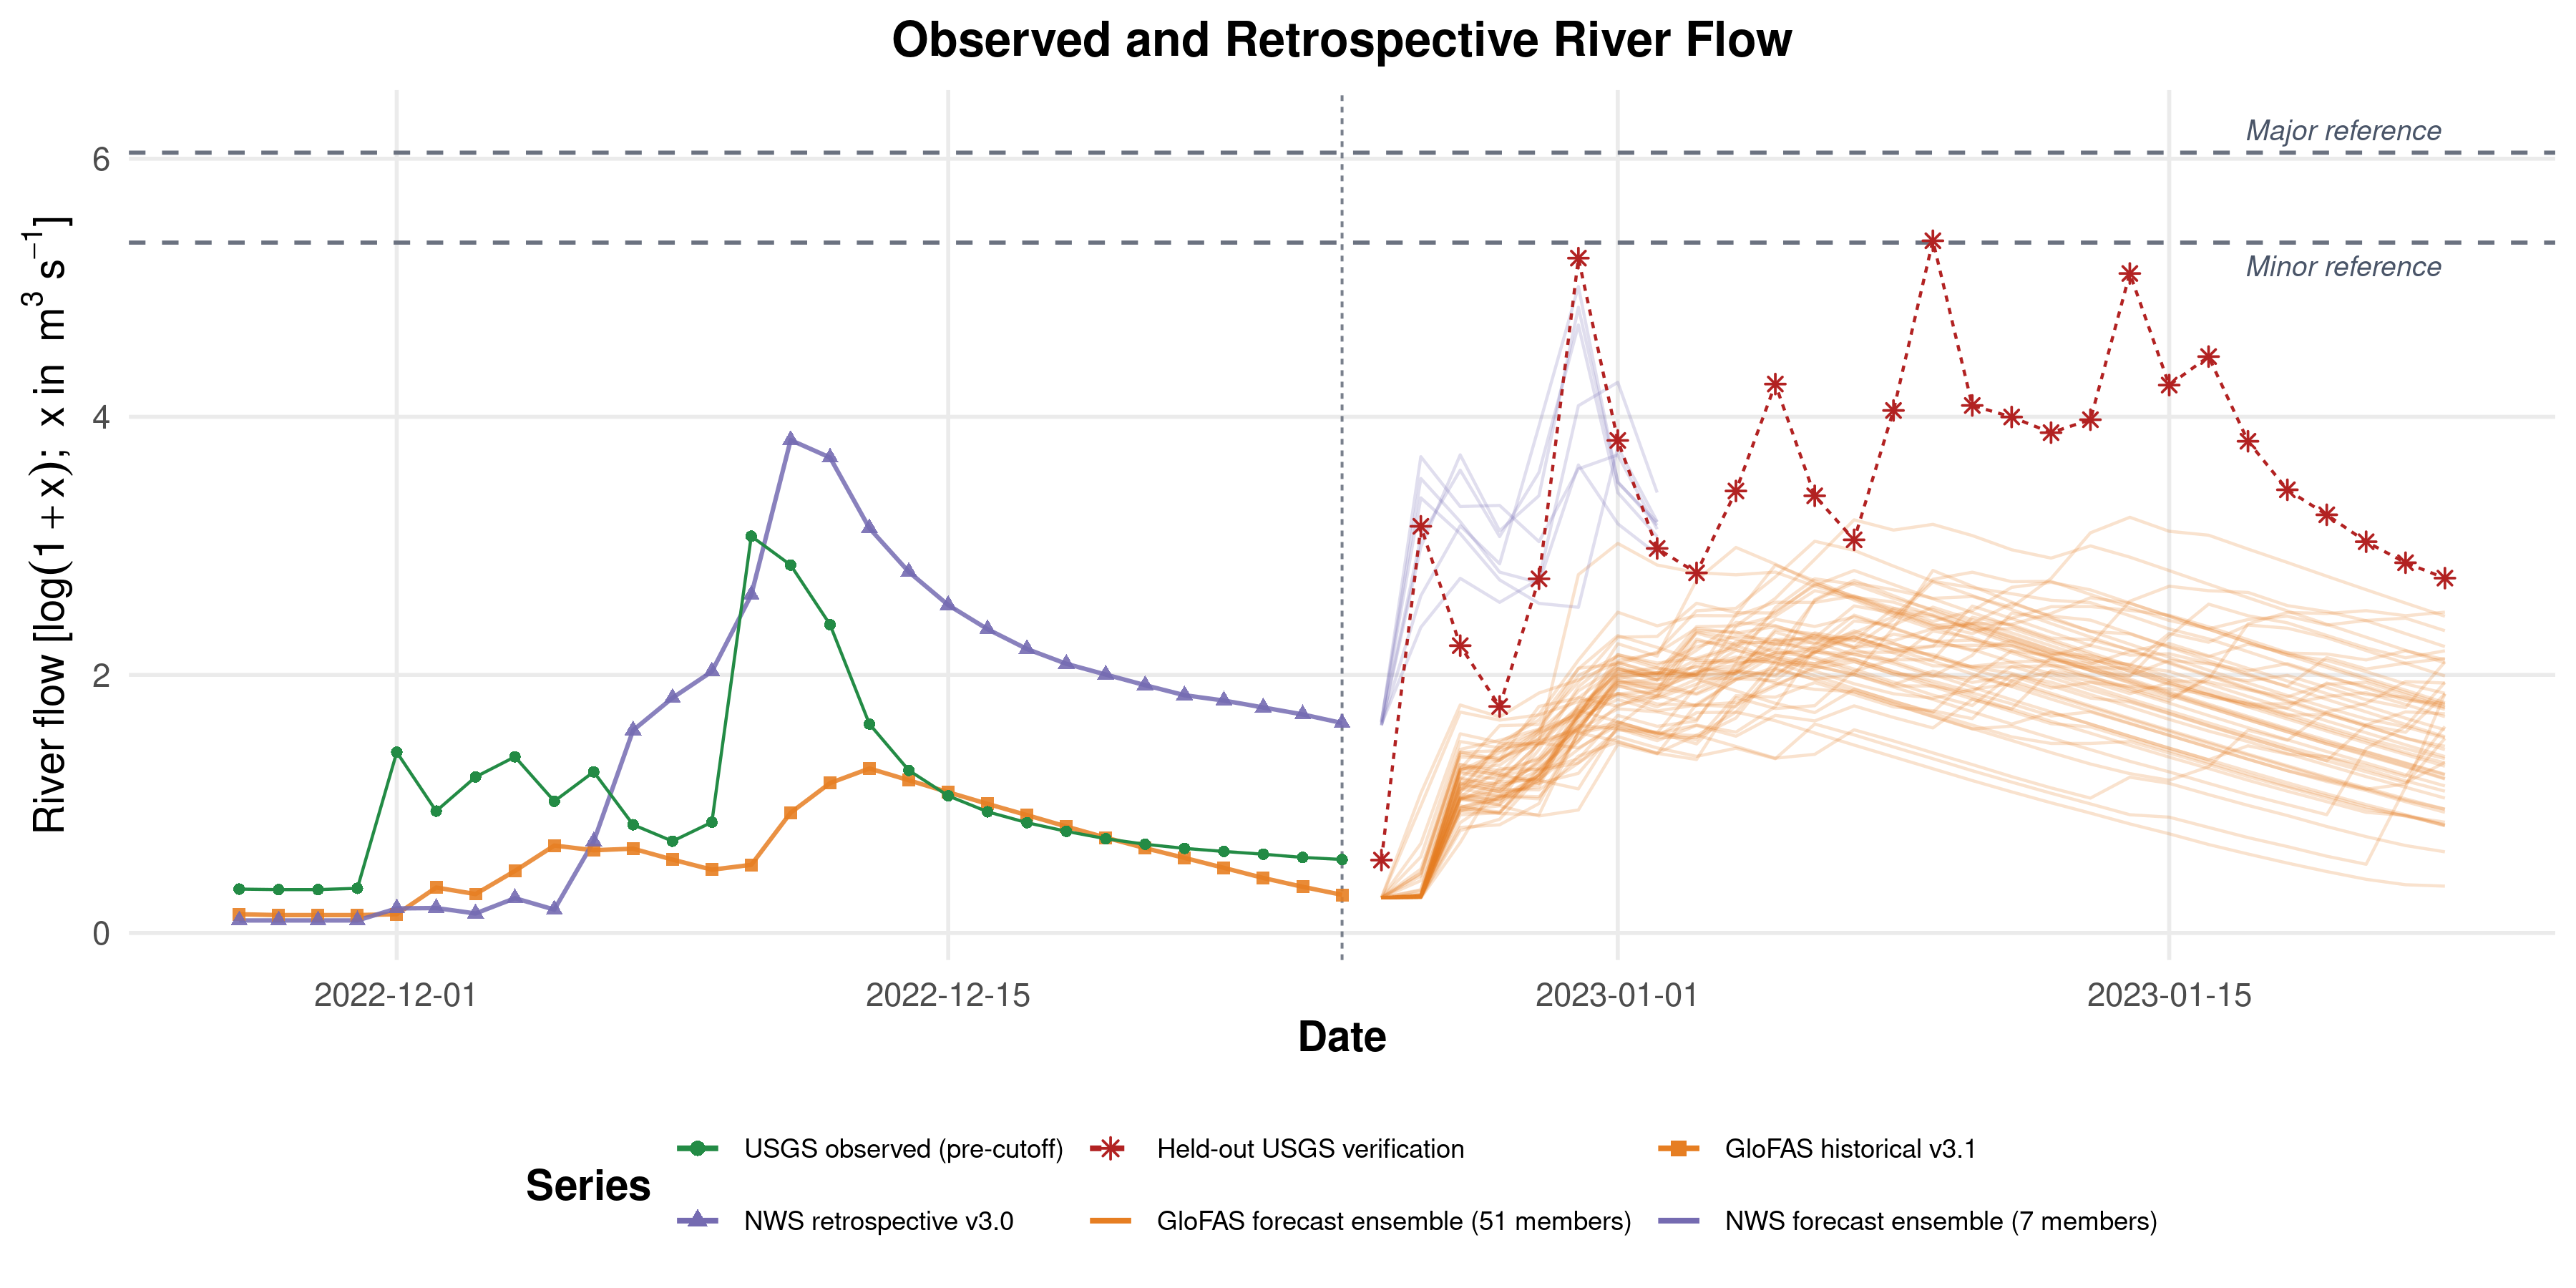
\includegraphics[width=450pt]{forecast_products_context.png}}
\caption{
Information available around the December 25, 2022 forecast origin, spanning November 27, 2022 through January 22, 2023 on the $\log(1+x)$ scale with $x$ in m$^3$/s. Before the origin, the panel shows USGS observations and the NWS and GloFAS retrospective products used for source-discrepancy learning; after the origin, it shows held-out USGS verification together with the operational NWS and GloFAS forecast ensembles. Horizontal dashed lines show approximate current-rating discharge equivalents of the current NWS minor and major stage categories at BTEC1/USGS 11160500. These levels provide magnitude references on the discharge scale.
}
\label{fig:ensembles}
\end{figure}

\section{BAYESIAN CORRECTION AND PREDICTIVE SYNTHESIS}
\label{sec:methodology}

For each target probability \(p_0\), the model learns a latent river-flow quantile from observations and source-specific products. The framework has two stages: dynamic correction combines the information channels within each quantile fit, and predictive synthesis combines output across those fits. Bold symbols denote vectors or matrices; their dimensions are stated when introduced. We write \(\mathbf I_r\), \(\mathbf 0_r\), and \(\mathbf 1_r\) for the \(r\)-dimensional identity matrix, zero vector, and one vector, respectively.

\subsection{Quantile Likelihood}
\label{subsec:exal}

The asymmetric Laplace (AL) distribution provides a working likelihood for Bayesian quantile inference \citep{yu2001bayesian, sriram2013theoretical}. We use its extended form, \(\operatorname{exAL}_{p_0}(\mu,\sigma,\gamma)\), developed by \citet{yan2025new}. Its location \(\mu\) is the \(p_0\)-quantile, \(\sigma>0\) controls scale, and \(\gamma\) provides additional skewness flexibility. To preserve the specified quantile, \(\gamma\) lies in an interval \((L_\gamma(p_0),U_\gamma(p_0))\) whose endpoints depend on \(p_0\). Appendix~\ref{app:augmentation} gives these endpoints and the latent-variable representation used for computation. This distribution defines the observation model; the state process below determines how its quantile evolves and is shared across sources.

\subsection{State-Space Model Specification}
\label{subsec:fullmodel}

For a fixed target quantile $p_0$, we use a state-space model for the transformed discharge \(\log(1+x)\). Its latent process spans the historical observation period and the forecast horizon defined by the origin \(T\). The latent river-flow quantile is represented by a trend-and-seasonal state \(\boldsymbol{\theta}_t \in \mathbb{R}^p\), observed through the loading vector \(\mathbf{F}_t\). Each external product family \(j\) has its own discrepancy state \(\boldsymbol{\delta}_t^j \in \mathbb{R}^p\), allowing that product to depart systematically from the observed river-flow series. A scalar transfer adjustment \(\zeta_t\) incorporates exogenous covariates \(\mathbf{x}_t \in \mathbb{R}^m\), whose time-varying effects are collected in \(\boldsymbol{\psi}_t \in \mathbb{R}^m\). Let \(\mathcal{J}=\{1,\ldots,J\}\) denote the set of external product families. For each \(j\in\mathcal{J}\), let \(\mathcal{I}_j=\{1,\ldots,I_j\}\) index forecast members and \(\mathcal{K}_j=\{1,\ldots,K_{(j)}\}\) index forecast lead times. Finally, define \(K_{\max}=\max_{j\in\mathcal{J}}K_{(j)}\), the maximum forecast horizon across all sources.

Conditionally on the states and channel parameters, the observation channels are independent and have the following distributions:
\begin{alignat}{3}
\text{Observed measurements:}\quad&
y_t^o
&\sim{}& \text{exAL}_{p_0}\!\left(\mathbf{F}_t' \boldsymbol{\theta}_t + \zeta_t, \sigma^0, \gamma^0\right),
&\qquad& 1 \le t \le T, \label{eq:unified_usgs}
\\
\text{Retrospective products:}\quad&
z_t^j
&\sim{}& \text{exAL}_{p_0}\!\left(\mathbf{F}_t'(\boldsymbol{\theta}_t + \boldsymbol{\delta}_t^j) + \zeta_t, \sigma^j, \gamma^j\right),
&\qquad& j \in \mathcal{J},\ 1 \le t \le T, \label{eq:unified_retro}
\\
\text{Forecast products:}\quad&
y_T^{j,i}(k)
&\sim{}& \text{exAL}_{p_0}\!\left(\mathbf{F}_{T+k}'(\boldsymbol{\theta}_{T+k} + \boldsymbol{\delta}_{T+k}^j) + \zeta_{T+k}, \sigma^j, \gamma^j\right),
&\qquad& j \in \mathcal{J},\ i \in \mathcal{I}_j,\ k \in \mathcal{K}_j, \notag
\\
\text{Trend and seasonal states:}\quad&
\boldsymbol{\theta}_t \mid \boldsymbol{\theta}_{t-1}
&\sim{}& \mathcal{N}\!\left(\mathbf{G}_t \boldsymbol{\theta}_{t-1}, \mathbf{W}_t^\theta\right),
&\qquad& 1 \le t \le T+K_{\max}, \label{eq:unified_theta}
\\
\text{Discrepancy states:}\quad&
\boldsymbol{\delta}_t^j \mid \boldsymbol{\delta}_{t-1}^j
&\sim{}& \mathcal{N}\!\left(\mathbf{G}_t \boldsymbol{\delta}_{t-1}^j, \mathbf{W}_t^{\delta^j}\right),
&\qquad& j \in \mathcal{J},\ 1 \le t \le T+K_{\max}, \label{eq:unified_delta}
\\
\text{Transfer adjustment:}\quad&
\zeta_t \mid \zeta_{t-1}, \boldsymbol{\psi}_{t-1}
&\sim{}& \mathcal{N}\!\left(\lambda \zeta_{t-1} + \mathbf{x}_t'\boldsymbol{\psi}_{t-1}, w_t^\zeta\right),
&\qquad& 1 \le t \le T+K_{\max}, \label{eq:unified_transfer}
\\
\text{Covariate-effect states:}\quad&
\boldsymbol{\psi}_t \mid \boldsymbol{\psi}_{t-1}
&\sim{}& \mathcal{N}\!\left(\boldsymbol{\psi}_{t-1}, \mathbf{W}_t^\psi\right),
&\qquad& 1 \le t \le T+K_{\max}. \notag
\end{alignat}

Here \(\mathbf{F}_t \in \mathbb{R}^{p}\), \(\mathbf{G}_t \in \mathbb{R}^{p\times p}\), \(\mathbf{W}_t^\theta \in \mathbb{R}^{p\times p}\), \(\mathbf{W}_t^{\delta^j} \in \mathbb{R}^{p\times p}\), \(\mathbf{W}_t^\psi \in \mathbb{R}^{m\times m}\), and \(w_t^\zeta \in \mathbb{R}_+\) is the scalar evolution variance for the transfer state \(\zeta_t\). The parameter \(\lambda \in \mathbb{R}\) governs persistence in the transfer adjustment, while \(\mathbf{x}_t'\boldsymbol{\psi}_{t-1}\) is the covariate contribution at time \(t\). During the forecast window, \(\mathbf{x}_{T+k}\) denotes the supplied covariate vector at lead \(k\). The notation \(y_T^{j,i}(k)\) denotes the \(k\)-step-ahead forecast issued at time \(T\) by member \(i\) of source \(j\).

The first two observation equations correspond to the pre-cutoff observation window, where the available channels are the observed USGS flow and the retrospective products. The third observation equation corresponds to the forecast window, where issued forecast products enter through the same source-specific discrepancy structure. The state-evolution equations define the roles of the dynamic components: \(\boldsymbol{\theta}_t\) carries the river-flow level and seasonal structure, \(\boldsymbol{\delta}_t^j\) captures systematic source-specific departures from the observations, and the transfer component maps exogenous covariates into the quantile process through \(\zeta_t\) and \(\boldsymbol{\psi}_t\). These are modeling roles; their forecast value is assessed through the specified comparisons in Subsection~\ref{subsec:comparisonspecifications}.

For each source and lead, the working likelihood multiplies the contributions of the available members. Their residual contributions are conditionally independent given the latent state and channel parameters; shared uncertain states induce dependence after integration. Member counts contribute information together with source scales and member-specific augmentation precisions, so the counts alone do not determine a fixed source-weight ratio. The observation scale and skewness have a common parameterization for retrospective and issued products, without an explicit lead index. Discrepancy states, evolution covariance, and source availability vary through the forecast window, allowing total predictive uncertainty to change. This parameter sharing is a parsimonious assumption; the specified likelihood does not explicitly represent residual member correlation or lead-dependent observation scale.

For prior specification and computation, collect the latent components in
\[
\boldsymbol\eta_t'=[\boldsymbol\theta_t',\ (\boldsymbol\delta_t^1)',\ldots,(\boldsymbol\delta_t^J)',\ \zeta_t,\ \boldsymbol\psi_t'],
\qquad q=(J+1)p+m+1.
\]
Let \(\mathcal J_0=\{0\}\cup\mathcal J\), with channel 0 denoting USGS and channels \(1,\ldots,J\) denoting the external source families. Appendix~\ref{app:stateconstruction} constructs the selector vectors and block matrices for this \(q\)-dimensional state. That compact representation is used by the algorithms; the equations above specify its scientific components.

\subsection{Prior Specification and Discounting}
\label{subsec:prioranddisc}
To complete the model we specify prior distributions for the initial states, the scale, and skewness parameters.
Following \citet{barata2021_flex_quantile}, for each channel-specific skewness parameter, we assign a truncated Student-\(t\) prior:
\[
\gamma^s \sim t_{(L_\gamma(p_0),U_\gamma(p_0))}(0,\phi^s,\nu^s), \qquad s\in\mathcal{J}_0,
\]
where \(\phi^s\) and \(\nu^s\) denote the scale and degrees of freedom hyperparameters, respectively. For the channel-specific scale parameters, we use inverse-gamma priors,
\[
\sigma^s \sim IG(a_{\sigma^s}, b_{\sigma^s}), \qquad s\in\mathcal{J}_0,
\]
with \(a_{\sigma^s}\) and \(b_{\sigma^s}\) as shape and scale hyperparameters. The full latent state is initialized as \(\boldsymbol{\eta}_0 \sim \mathcal{N}(\mathbf{m}_0, \mathbf{C}_0)\), with \(\mathbf{m}_0 \in \mathbb{R}^{q}\) and \(\mathbf{C}_0 \in \mathbb{R}^{q\times q}\). This initial prior covers the shared trend-and-seasonal quantile block, the source-specific discrepancy blocks, and the transfer block.

Component discount factors \citep{prado2021time} control state-evolution variances. Values lie in \((0,1]\): a value of 1 suppresses evolution for that component, while smaller values allow greater temporal adaptation. In the forecast window, an inverse-Wishart prior stabilizes the evolution covariance around \(c\mathbf W_T\), the covariance learned at the origin and multiplied by a positive scale \(c\). A positive parameter \(\epsilon\) gives this anchor weight \(\epsilon/(1+\epsilon)\) in the posterior mean; the remaining weight is assigned to the expected state-innovation covariance. Appendix~\ref{app:forecastcovariance} gives the full specification and dimensions. Subsection~\ref{subsec:specification} gives the application settings.

\subsection{Posterior Computation}
\label{subsec:postinf}

The reported fits use mean-field VB. Conditional on the exAL augmentation variables, the observations are Gaussian and the latent state follows a Gaussian evolution model. This structure permits a joint Gaussian approximation for the state trajectory, computed by variational filtering and smoothing. The remaining factors describe the observation-specific augmentation variables and each channel's scale and skewness parameters.

Coordinate-ascent iterations cycle through three groups of updates. Variational filtering and smoothing update the state means and covariances using expected observation precisions and precision-weighted offsets from the likelihood factors. Generalized inverse-Gaussian and positive-truncated normal updates refresh the augmentation factors. A VB Laplace--Delta (VB-LD) update approximates the joint scale and skewness factor for each channel: the Laplace approximation matches the mode and curvature on an unconstrained parameterization, and a second-order Delta approximation supplies the nonlinear expectations needed by the other updates \citep{wang2013nonconjugatevb}. The iterations monitor changes in the evidence lower bound (ELBO), state, scale, and skewness after required minimum update counts. Algorithms~\ref{alg:Alg3} and \ref{alg:Alg4} give the update sequence and state recursions; Appendix~\ref{app:vblad} gives the approximation formulas.

This adaptation extends the flexible DQLM approach of \citet{barata2021_flex_quantile}, whose importance-sampling treatment of non-conjugate parameters fixes the scale using an AL fit. The Laplace--Delta updates approximate scale and skewness jointly. They provide the deterministic posterior approximation used throughout the comparisons below. Algorithms~\ref{alg1} and \ref{alg:Alg2} give conditional sampling equations for the historical observation model. All reported posterior summaries use VB; its accuracy relative to a full-model Markov chain Monte Carlo (MCMC) posterior has not been assessed.

Separate target quantiles can be fitted in parallel using the estimation routines in the \texttt{exdqlm} package \citep{deleon2026exdqlm}. With the model-ready observations, retrospective products, forecast products, and covariates prepared, representative publication runs for the seven-quantile set take about two hours end-to-end on a Linux server with 64 cores and 503 GiB of RAM. This is combined wall-clock time for fitting and forecasting; those stages were not timed separately. Runtime depends on the hardware, implementation, series length, and state dimension, with repeated filtering and smoothing accounting for the main computational cost.

\subsection{Posterior Predictive Synthesis Across Quantiles}
\label{subsec:quantilesynthesis}

The source-aware model is fitted separately at probabilities \(0<\tau_1<\cdots<\tau_L<1\), setting \(p_0=\tau_\ell\) in fit \(\ell\). These fits need not produce an ordered set of quantiles. A separate post-processing step constructs one marginal predictive distribution at each time from their predictive draws, without changing the fitted state-space models.

Let \(Y_{\ell,t}^{(r)}\), \(r=1,\ldots,R\), denote predictive draws from fit \(\ell\), and let \(q_{\ell,t}\) be their empirical \(\tau_\ell\)-quantile. First, isotonic regression \citep{barlow1972} orders these anchors:
\[
\mathbf m_t^*=\underset{m_1\le\cdots\le m_L}{\arg\min}
\sum_{\ell=1}^L(q_{\ell,t}-m_\ell)^2.
\]
Each fit's draws are shifted by \(m_{\ell,t}^*-q_{\ell,t}\). Write \(Q^{\rm adj}_{\ell,t}\) for the empirical quantile function of the shifted draws. For \(\tau_\ell<u<\tau_{\ell+1}\), the initial synthesized curve is
\[
Q_t^{\rm init}(u)=(1-w)Q^{\rm adj}_{\ell,t}(u)+wQ^{\rm adj}_{\ell+1,t}(u),
\qquad w=\frac{u-\tau_\ell}{\tau_{\ell+1}-\tau_\ell}.
\]
Below \(\tau_1\) and above \(\tau_L\), it uses the adjusted quantile functions of the lowest and highest fitted probabilities, respectively. Thus the blend uses the predictive distributions, including their tails, as well as their fitted quantile anchors.

We evaluate this curve on a dense probability grid and sort its values, applying monotone rearrangement \citep{chernozhukov2010} to obtain a nondecreasing quantile function \(\widetilde Q_t\). Inverse cumulative distribution function (CDF) sampling then gives
\[
\widetilde Y_t^{(r)}=\widetilde Q_t(U_t^{(r)}),\qquad
U_t^{(r)}\sim\operatorname{Uniform}(0,1).
\]
The resulting sample defines the per-time marginal predictive distribution used for the predictive means, pointwise intervals, quantiles, and continuous ranked probability score (CRPS) calculations. The implementation evaluates the initial curve at 1,001 internal grid points, applies rearrangement, and produces 2,000 inverse-CDF draws per time; interpolation is constant beyond the endpoint grid values. The outer fitted predictive distributions supply the tails beyond the 0.05 and 0.95 anchors, including the limits of the reported central 95\% intervals. These limits are not separately fitted 0.025 and 0.975 quantile models. The synthesis is marginal in time: lines connecting displayed sample values should be read as predictive sample traces, without a jointly specified temporal dependence model for those synthesized traces.

We separately assess the own-fit predictive anchors, their isotonic projection, and the final synthesized quantiles using targeted check loss and crossing counts. Own-fit anchors use sample type 7, as in the synthesis construction. They are predictive quantiles from the individual fits, distinct from latent fitted locations. The seven anchors alone do not define a complete predictive distribution for a pre-synthesis CRPS comparison.

\section{APPLICATION SPECIFICATION AND EVALUATION}
\label{sec:evaluation}

\subsection{Dynamic Components and Numerical Settings}
\label{subsec:specification}

The application uses a local level to represent persistent flow conditions, two approximately annual and semiannual rotations to describe recurring within-year variation, and a slower rotation to permit multi-year variation. The slower component was retained as an exploratory representation of multi-year variability. Its period is a model-specification choice, and we do not assign it to a particular physical climate mechanism. Each source discrepancy has the same seven-state level-and-seasonal structure, allowing source differences to vary at these time scales.

For daily time steps, the fitted seasonal constructor uses a base period \(P=363.5854\) days and frequency multipliers \(h_1=1\), \(h_2=2\), and \(h_3=1/6.8068493\). The daily angular frequencies are \(\omega_a=2\pi h_a/P\), with rotation matrix
\[
\mathbf R(\omega)=
\begin{bmatrix}\cos\omega&\sin\omega\\-\sin\omega&\cos\omega\end{bmatrix}.
\]
The corresponding periods are approximately 363.59, 181.79, and 2474.87 days; the last is about 6.78 calendar years, or 81.3 months. These are the periods of the fitted daily rotations. With \(\mathbf E_2=(1,0)'\), the observation loading and transition are
\[
\mathbf F_t=(1,\mathbf E_2',\mathbf E_2',\mathbf E_2')',\qquad
\mathbf G_t=\operatorname{BlockDiag}\{1,\mathbf R(\omega_1),\mathbf R(\omega_2),\mathbf R(\omega_3)\},
\]
so \(p=7\), \(\mathbf F_t\in\mathbb R^7\), and \(\mathbf G_t\in\mathbb R^{7\times7}\).

The transfer vector has \(m=12\) predictors. In addition to precipitation, soil moisture, and the first GDPC score, it includes squared precipitation, squared soil moisture, their interaction, and separate one-, two-, and three-day lags of precipitation and soil moisture. Each engineered predictor is divided by its historical standard deviation without centering. These terms permit delayed and nonlinear covariate contributions within the linear state-space formulation. The scalar transfer state \(\zeta_t\) adds persistence through \(\lambda\). With two external source families, the full model therefore has \(q=3(7)+12+1=34\) latent states. Table~\ref{tab:components_23_31} summarizes the three base-input coefficients.

For prior hyperparameters (see Subsection~\ref{subsec:prioranddisc}), we specify \(\phi^s = 10^6\), \(\nu^s = 1\), and \(a_{\sigma^s} = b_{\sigma^s} = 10^{-6}\) for all \(s\in\mathcal{J}_0\), reflecting diffuse prior beliefs for both the USGS observation channel and the external product channels. Sensitivity analyses for \(\phi^s \in \{10^1, 10^3, 10^6\}\) and \(b_{\sigma^s} \in \{10^{-1}, 10^{-3}, 10^{-6}\}\) showed no noticeable impact on model fit.

We choose discount factors componentwise to reflect each component's time scale and role. Recall that, in the discount-factor formulation \citep{prado2021time}, a smaller value \(d \in (0,1]\) for a given state parameter implies larger state-evolution variance and therefore greater adaptability of that component. The selected specifications use high, near-one discount factors for the trend, seasonal, discrepancy, transfer, and covariate-effect states. These values preserve persistent long-run behavior while allowing slow adaptation across the multi-decade observation window. Table~\ref{tab:no_refit_settings} gives their exact values for the five reference fits; the reproducibility bundle records all 45 model--origin specifications. The discrepancy factor multiplies the associated component discount, so it is distinguished from the resulting effective discount.

The transfer-persistence parameter \(\lambda\) was selected in a preliminary one-dimensional calibration step for the reference extended-likelihood multivariate specification with an active transfer component. To avoid confounding transfer persistence with state-evolution adaptability, the component discount factors were held fixed during this step. We considered the grid \(\lambda \in \{0.60,0.61,\ldots,0.99\}\) and compared candidate values using CRPS for the median-quantile model over the pre-cutoff observational window at the representative December 25, 2022 origin, which has the longest pre-origin archive among the rolling-origin cases. The selected value was \(\lambda=0.97\), which was then held fixed across the reported quantile levels and forecast origins. The resulting fixed persistence setting is used in the reported comparisons.

For the forecast-window covariance prior, the parameter \(\epsilon\) controls the prior weight assigned to the covariance structure learned before the cutoff. Smaller values give a weaker anchor and allow greater adaptation during forecast propagation, while larger values retain more of the pre-cutoff covariance structure. For the representative December 25, 2022 selected specification, we set \(\epsilon=1\) and \(c=1\). These settings stabilize short-horizon forecast propagation while allowing the forecast-window state evolution to adapt during a winter origin with substantial rainfall-driven uncertainty.

\subsection{Forecast Origins and Product Alignment}

The evaluation uses five forecast origins spanning relatively low-flow conditions and winter high-flow episodes: January 23, November 12, and December 21, 2021, and May 11 and December 25, 2022. For each origin, a model-ready dataset aligns the observations, retrospective products, issued ensembles, and covariate paths. These five cases cover contrasting hydrological settings; they do not constitute a continuous daily hindcast. The separated origins also avoid repeatedly scoring strongly overlapping forecast windows from one episode. Extending the evaluation requires recovering and aligning the corresponding historical product versions, spatial extractions, members, and lead times.

The fitting window includes USGS observations and retrospective products through \(T\). Forecast inference uses the external ensembles for their available leads and the supplied transfer covariates. USGS values after \(T\) supply verification. GloFAS issues daily forecasts. For the hourly NWS product, the input construction retains the latest available issuance for each target time and member at the origin, then aggregates the retained hourly values to daily resolution. The comparison uses eight daily leads for the common NWS horizon and 28 leads for the GloFAS horizon, with each source entering only where its forecast members are available.

\subsection{Comparison Specifications}
\label{subsec:comparisonspecifications}

We compare nine Bayesian variants of the common state-space framework. These variants differ only in three respects: the observation likelihood, whether the synthesis uses only the USGS observation channel or all source channels jointly, and whether the transfer component remains active during the forecast window. We summarize them with the label \(L\)-\(S\)-\(T\), where \(L\in\{\mathrm{N},\mathrm{AL},\mathrm{exAL}\}\) denotes a Gaussian, asymmetric Laplace, or extended asymmetric Laplace observation likelihood, \(S\in\{\mathrm{U},\mathrm{M}\}\) indicates whether the synthesis is univariate or multivariate, and \(T\in\{\mathrm{T0},\mathrm{T1}\}\) indicates whether the transfer component is suppressed or retained during the forecast window.

For the AL and exAL variants, we fit the framework separately at seven target quantile levels: \(0.05\), \(0.20\), \(0.35\), \(0.50\), \(0.65\), \(0.80\), and \(0.95\). The Gaussian variants correspond to normal dynamic linear models. Forecast skill is evaluated from the resulting posterior predictive distributions by the mean CRPS. The comparisons use the VB procedure described in Subsection~\ref{subsec:postinf}.

For the predictive illustration and component summaries, we use exAL-M-T1: the extended likelihood, all source channels, and the active transfer component. This is the reference specification selected from the 28-day comparison reported in Section~\ref{sec:forecastvalidation}. Its single-origin display is illustrative; the tables summarize performance across the five origins.

Table~\ref{tab:comparisonroles} relates the model comparisons to their questions. The nine variants are a selected set of configurations, not a fully crossed factorial experiment. A difference between two fitted configurations describes their performance under the reported fitting policies; it need not equal the benefit achievable after separately redesigning or retuning either configuration. The structural sensitivity analysis in Appendix~\ref{app:he3ablation} likewise retains the reference settings when components are removed.

To assess the fitting explanation for poor scores, we audit the saved terminal criteria, iteration budgets, parameter updates, numerical guards, and sampling outcomes for the configurations in both comparisons. Completion messages alone do not establish convergence. The audit distinguishes recorded satisfaction of the stopping criteria, exhaustion of the iteration budget without established joint convergence, and unavailable joint-criterion evidence; Appendix~\ref{app:fitdiagnostics} reports the findings.

\begin{table}[htbp]
\caption{Questions addressed by the internal comparisons.}
\label{tab:comparisonroles}
\centering
\begin{tabular}{p{0.22\linewidth}p{0.31\linewidth}p{0.39\linewidth}}
\hline
Modeling role & Reported comparison & Interpretation \\
\hline
Observation-distribution flexibility & N, AL, and exAL with matching source and transfer labels & Changes the likelihood family; gains may depend on the source and transfer configuration. \\
External source information & U versus M within a likelihood and transfer setting & Compares gauge-only and source-inclusive configurations, including their discrepancy states. \\
Forecast-window covariate contribution & T0 versus T1 within a multivariate likelihood & Suppresses or retains transfer during forecasting; the transfer component is fitted historically in both. \\
Level, seasonal, and transfer structure & Full exAL-M-T1 versus one-component removals & Measures sensitivity to removing a structural block under inherited reference settings. \\
\hline
\end{tabular}
\end{table}

\subsection{External Forecasting References}
\label{subsec:externalreferences}

We add three references with distinct practical roles. Seasonal climatology (CLIM-SEASONAL) is an empirical distribution of historical USGS flow on the transformed scale. For each forecast date, it uses observations from May 29, 1987 through the origin within \(\pm15\) calendar positions of the target month and day. Positions follow a circular calendar based on the leap year 2000, retaining a separate February 29 position. This provides a season-specific distribution without using a hydrological forecast product. Persistence (PERSISTENCE) is a point mass at the last observed transformed discharge, \(\log(1+x_T)\), repeated at every lead. Its CRPS is the absolute forecast error.

The third reference, EMOS-GLOFAS, is a truncated-normal EMOS correction of GloFAS \citep{gneiting2005emos, thorarinsdottir2010emos}. Hydrological use of EMOS motivates this established post-processing comparator \citep{hemri2015multivariate}. At each lead, its predictive distribution for transformed discharge is normal truncated below zero, with pre-truncation location and variance
\[
\mu=a+b\bar g,\qquad \sigma^2=c+d s_g^2,
\]
where \(\bar g\) and \(s_g^2\) are the mean and unbiased sample variance of the 51 transformed GloFAS members. The parameters satisfy \(b,d\geq0\) and \(c>0\).

We fit a separate parameter vector for each lead using up to 365 preceding daily issuances, retaining only cases issued before the origin and verified by that origin. Training is restricted to the compatible GloFAS version family, with the version 2 to version 3 transition on May 26, 2021, and requires at least 100 cases per lead. Four deterministic starts use bounded L-BFGS-B optimization to minimize the analytic truncated-normal training CRPS; we retain the converged solution with the lowest objective. The training cases, numerical scaling and bounds, fitted parameters, convergence results, and boundary checks are retained in the reproducibility outputs. This comparator corrects one product through ensemble location and spread; it does not use the quantile state-space or transfer construction.

\subsection{Predictive Scoring by CRPS}
\label{subsec:modelselection}

For predictive scoring, we use CRPS \citep{gneiting2007strictly} to compare forecast-window predictive distributions. It also supplies the preliminary persistence-calibration criterion in Subsection~\ref{subsec:specification}. The CRPS is negatively oriented, so smaller values are better, and it is a proper score for predictive distributions that rewards both calibration and sharpness.

For a predictive distribution \(G\) with quantile function \(Q_G\) and an observation \(y\), the CRPS is defined as
\[
\text{CRPS}(y, G) = 2 \int_0^1 \rho_u\!\left(y - Q_G(u)\right)\, du,
\qquad
\rho_u(v) = v\big(u - \mathbf{1}\{v<0\}\big),
\]
where \(\rho_u\) is the quantile score, or check loss. Thus, the CRPS is a natural score in the context of quantile estimation. For an empirical predictive distribution represented by sample values \(\widetilde Y_t^{(1)},\ldots,\widetilde Y_t^{(S)}\), we approximate the integral by evaluating the empirical quantile function on the grid \(u_s=s/(S+1)\), \(s=1,\ldots,S\). Let \(\widetilde Y_{t,(1)} \leq \cdots \leq \widetilde Y_{t,(S)}\) be the corresponding ordered sample values. Then
\[
\widehat{\mathrm{CRPS}}(y_t,G_t)
= \frac{2}{S}\sum_{s=1}^S
\rho_{u_s}\!\left(y_t-\widetilde Y_{t,(s)}\right).
\]
The same calculation is used for synthesized posterior predictive samples and for raw forecast ensembles, with \(S\) equal to the number of available sample draws or ensemble members at that lead. If the predictive distribution is a point mass at \(x\), the CRPS reduces to \(|y-x|\); averaging this quantity across forecast cases gives the mean absolute error. CRPS is also used in the preliminary pre-cutoff calibration of the transfer-persistence parameter \(\lambda\), as described in Subsection~\ref{subsec:specification}.


Mean scores average the daily scores within each origin and horizon, on the \(\log(1+x)\) discharge scale used for fitting. We also report check loss \(\rho_\tau\) at the seven fitted quantile probabilities, using the corresponding synthesized predictive quantiles. These targeted scores describe performance at individual parts of the distribution alongside the distribution-wide CRPS comparison.

To give these scores a reference point, we also report the CRPS skill score (CRPSS) relative to seasonal climatology \citep{wilks2019statistical},
\[
\mathrm{CRPSS}=1-\frac{\overline{\mathrm{CRPS}}_{\rm method}}{\overline{\mathrm{CRPS}}_{\rm climatology}}.
\]
The numerator and denominator average over the same forecast cases and horizon. Positive values improve on climatology, zero indicates equal mean scores, and negative values indicate poorer performance. The aggregate skill score is computed from the ratio of aggregate mean scores, not the average of origin-specific ratios.

For the three added references, predictive quantiles at \(u_s=s/2001\), \(s=1,\ldots,2000\), enter the same numerical score calculation. Seasonal climatology uses the empirical inverse CDF without interpolation, persistence repeats its single value, and EMOS uses the fitted truncated-normal inverse CDF. Original model and raw-product scores are retained. The external comparison uses the same verification dates, eight-day and 28-day horizons, and transformed discharge scale.

\subsection{Distribution Scores and Predictive Calibration}
\label{subsec:distributionchecks}

To distinguish numerical scoring from the finite predictive representation, we additionally score the equally weighted empirical distribution \(G_m=m^{-1}\sum_{i=1}^m\delta_{x_i}\) exactly. Writing \(A=m^{-1}\sum_i|x_i-y|\) and \(D=\sum_{i<j}|x_i-x_j|\), its CRPS is
\[
\mathrm{CRPS}(G_m,y)=A-\frac{D}{m^2}.
\]
The quantile-grid approximation above equals this value plus \(D/[m^2(m+1)]\). Thus the two calculations score the same stored values using different finite-sample formulas \citep{zamo2018crps}. The new comparison uses the exact empirical-distribution score for all 14 methods, including the frozen 2,000-value climatology and EMOS quantile grids. Its CRPSS denominator is the exact score of that same climatology representation on matching cases and scale. Existing quantile-grid tables retain their original definition.

Stored sample sizes differ: the AL/exAL syntheses contain 2,000 inverse-CDF draws, the Gaussian univariate model 64 draws, the Gaussian multivariate models 48 draws, and raw GloFAS and NWS 51 and seven members. As a separate finite-sample sensitivity, we report \(A-D/[m(m-1)]\), whose expectation equals the parent-distribution CRPS for independent identically distributed draws \citep{ferro2014fair}. Independence is an additional working assumption for physical ensemble members; this sensitivity does not establish ensemble exchangeability or posterior accuracy. It is inapplicable to deterministic grids and point masses, and no adjusted CRPSS is reported.

Quantile reliability records the frequencies of \(y<q_\tau\) and \(y\leq q_\tau\), with exact ties counted separately. For the four principal quantile competitors we retain the predictive quantiles used in the existing check-loss analysis. Newly derived stochastic-model quantiles use sample type 8; raw ensembles and deterministic grids use the empirical generalized inverse. The displayed model ribbons use type-8 limits, with the selected multivariate limits checked against their existing exports. Central 95\% predictive intervals are evaluated as closed intervals \([l,u]\), with lower misses, coverage and upper misses forming an exact partition. We report mean width and the proper interval score
\[
\mathrm{IS}_{0.05}(l,u;y)=(u-l)+40(l-y)\mathbf1\{y<l\}+40(y-u)\mathbf1\{y>u\}.
\]
This assesses observation prediction, separately from the approximate parameter-posterior intervals.

We also evaluate discharge in m$^3$/s by applying \(\exp(x_i)-1\) to each stored predictive value before computing means and distribution scores. Targeted quantiles and interval endpoints are inverse-transformed from their declared log-scale values, preserving their forecast events. The stored predictive support is retained without truncation, so this analysis also reveals sensitivity to extreme tails. Comparisons use 140 verification cases over 28 days or 40 over eight days, always with complete matching dates. The five origins support descriptive calibration comparisons; successive daily cases are not treated as independent replicates for significance claims.

\section{RESULTS}
\label{sec:forecastvalidation}

\subsection{Predictive Synthesis Illustration}
\label{subsec:synthillustration}

Figure~\ref{fig:synth1} shows the synthesized posterior predictive distribution for the December 25, 2022 origin, under the exAL-M-T1 reference specification. The predictive ribbon includes observation-level variation as well as uncertainty propagated through the model and the quantile-synthesis step.

\begin{figure}[!htbp]
\centering
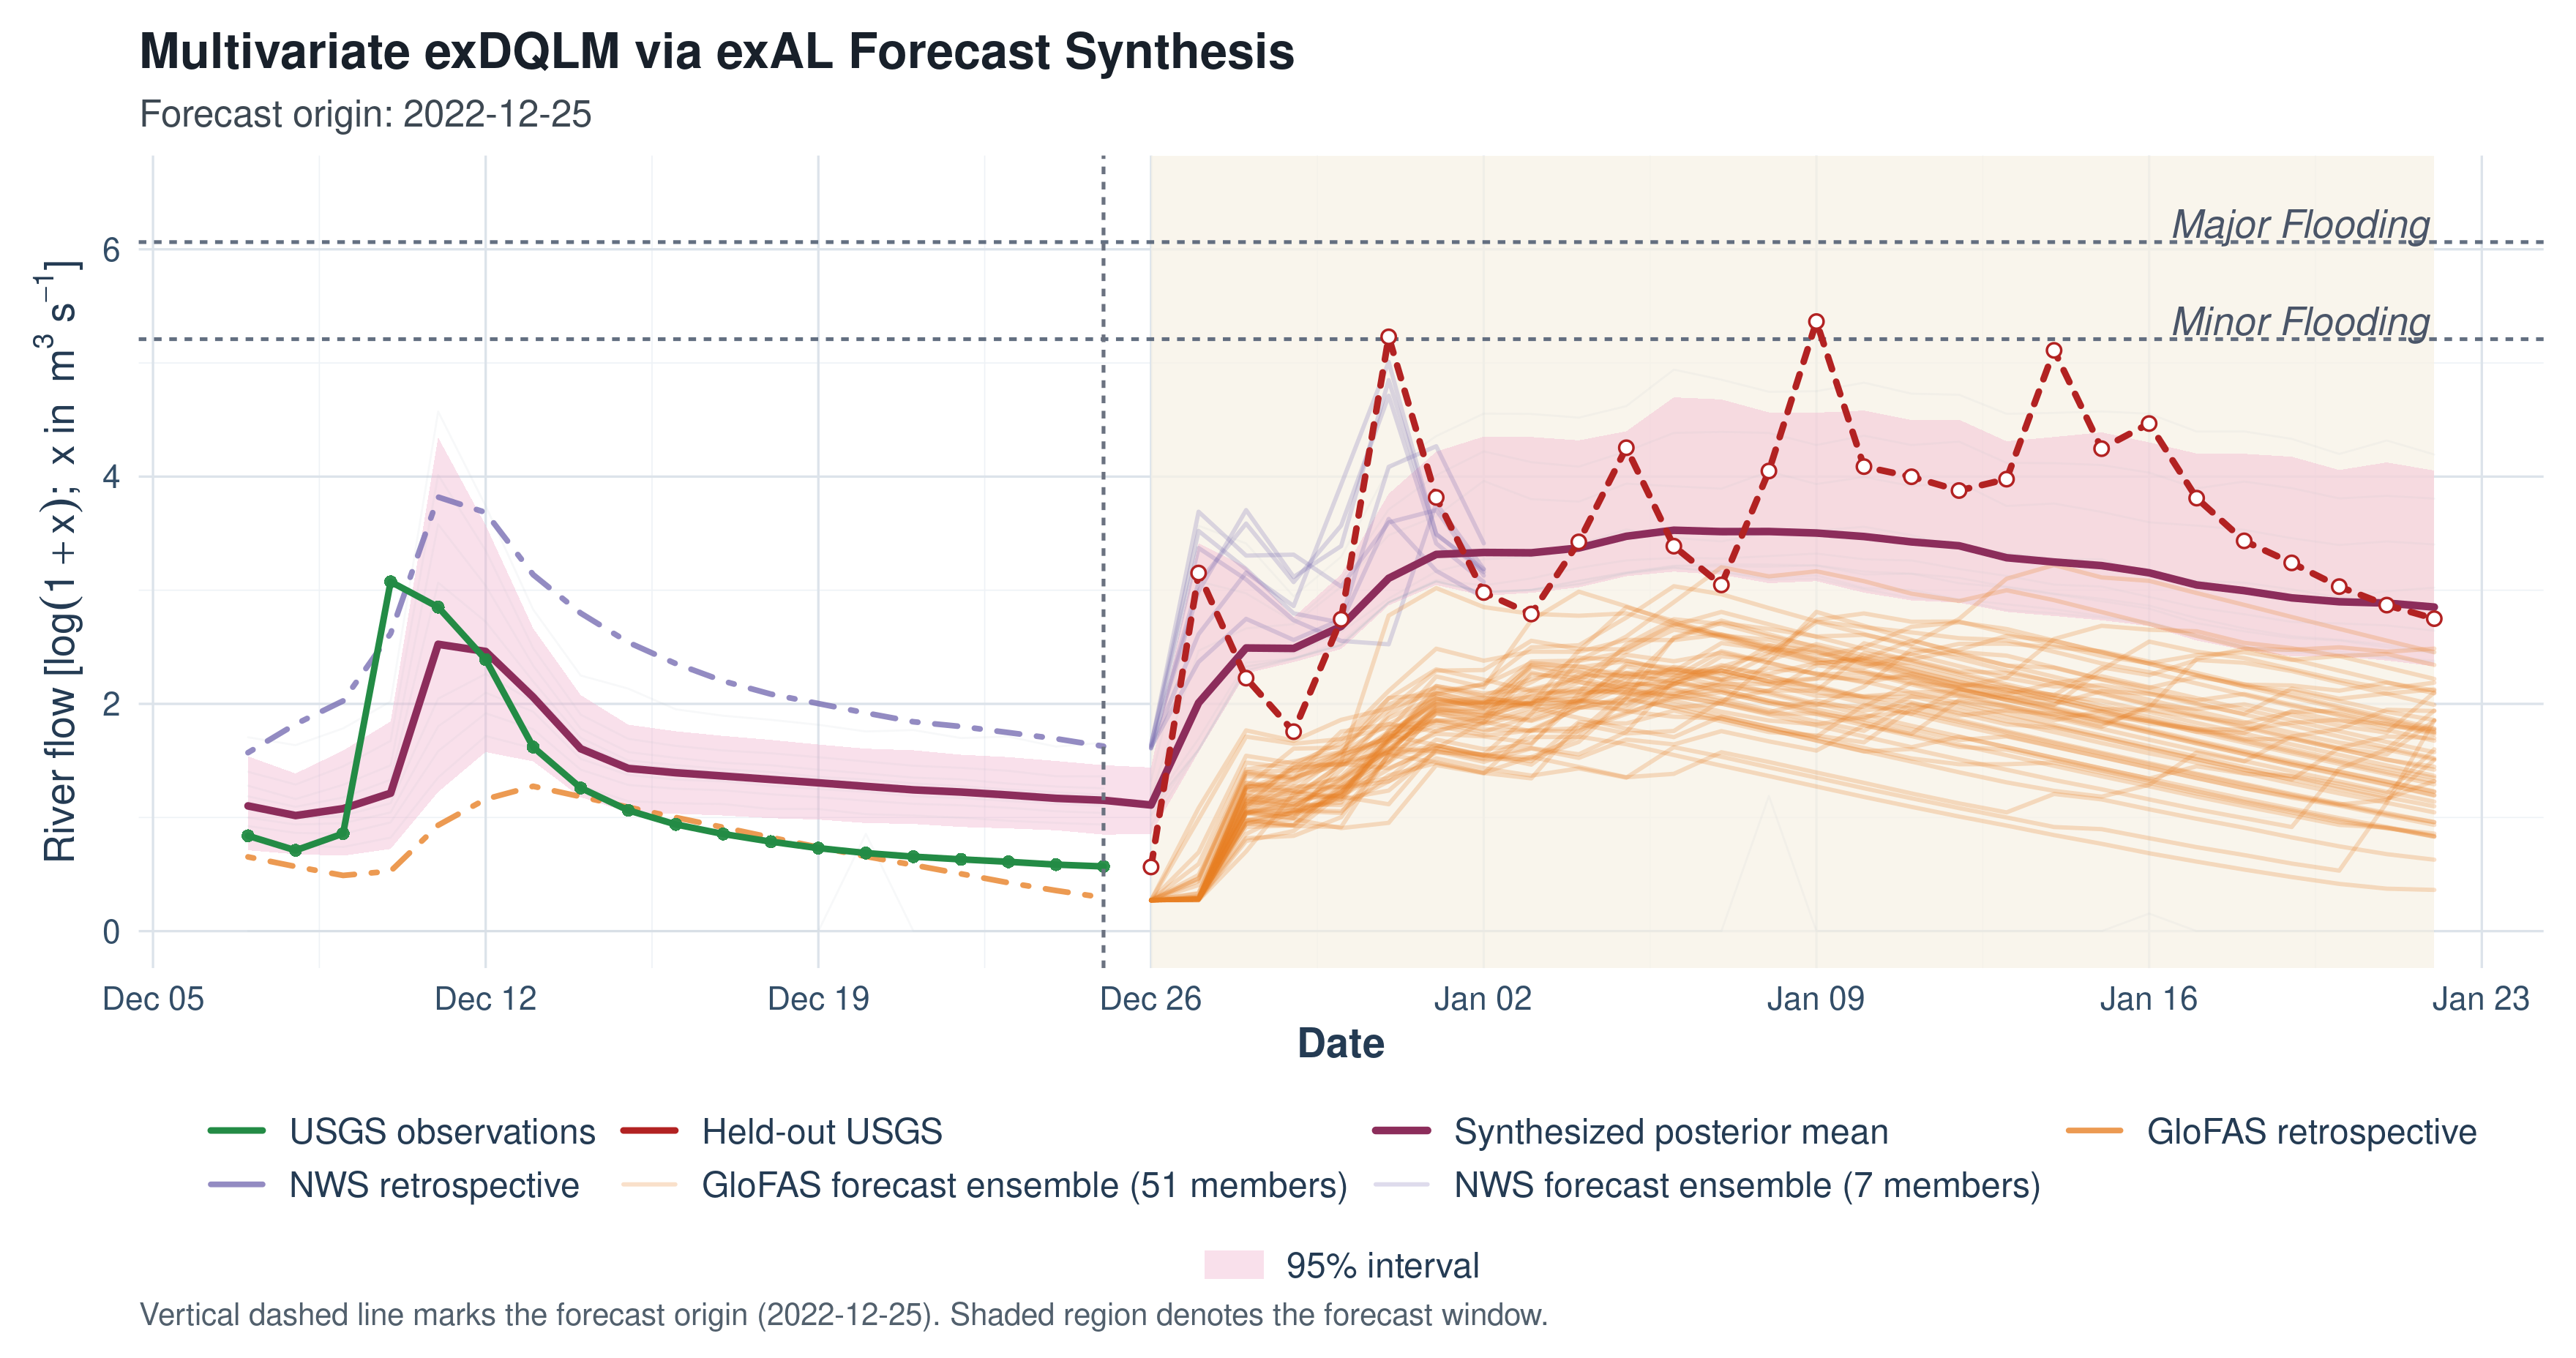
\includegraphics[width=450pt]{cutoff_2022_12_25_multivariate_synthesis_with_reference_ensembles.png}
\caption{
Synthesized posterior predictive distribution for river flow on the $\log(1+x)$ scale, with $x$ measured in m$^3$/s, at the December 25, 2022 forecast origin under the exAL-M-T1 model. Observed USGS measurements before the origin are shown in green, and held-out USGS verification after the origin is shown in red. The pink ribbon is the pointwise central 95\% predictive interval (2.5th--97.5th percentiles), and the dark line is the predictive mean on the \(\log(1+x)\) scale. The ten thin traces connect synthesized predictive sample values. The origin line marks \(T\), and the first forecast lead is \(T+1\). Raw retrospective and forecast products are shown for context. Horizontal guides mark discharge references of approximately 182 and 429~m$^3$/s.
}
\label{fig:synth1}
\end{figure}
The predictive mean and interval change across the forecast window as the source forecasts, their corrections, and the transfer inputs evolve. Their position relative to the discharge-reference levels provides a flow-magnitude interpretation of this forecast. The ribbon is a pointwise predictive interval, not an interval for a fitted quantile location. Appendix Figure~\ref{fig:synth2} gives the corresponding univariate reference, which retains transfer covariates and excludes the external source channels. Appendix Figures~\ref{fig:synthsupport_20210123}, \ref{fig:synthsupport_20211112}, \ref{fig:synthsupport_20211221}, and \ref{fig:synthsupport_20220511} give the remaining multivariate origins.

\subsection{Comparative Forecast Performance}
\label{subsec:benchmarkresults}

Table~\ref{tab:benchmark_crps_models} reports mean 28-day forecast-window CRPS. The multivariate rows use all available source channels, including NWS forecast information over the leads for which it is available, and the AL/exAL rows are posterior predictive syntheses assembled from the seven fitted quantile-specific models. The raw GloFAS product is included as the horizon-compatible 28-day raw reference; raw NWS is handled in the separate eight-day comparison because the archived NWS forecasts provide only eight valid daily leads for these origins.

\begin{table*}[htbp]
\centering
\renewcommand{\arraystretch}{1.08}
\begin{threeparttable}
\caption{Mean forecast-window CRPS by model family and cutoff across the five rolling-origin evaluation folds. Lower values are better; bold indicates the lowest CRPS within each cutoff column.}
\label{tab:benchmark_crps_models}
\begin{tabular*}{\textwidth}{@{\extracolsep{\fill}} >{\ttfamily}l r r r r r}
\toprule
Model label & 01/23/2021 & 11/12/2021 & 12/21/2021 & 05/11/2022 & 12/25/2022 \\
\midrule
\multicolumn{6}{l}{\textit{Raw forecast products}} \\
RAW-GLOFAS & 0.40366 & 0.16957 & 0.68246 & 0.27227 & 1.56006 \\
RAW-NWS & 0.83037 & 1.37192 & 0.28118 & 0.28366 & \textbf{0.55680} \\
\midrule
\multicolumn{6}{l}{\textit{Bayesian benchmark variants}} \\
N-U-T1 & 0.33592 & 0.17059 & 1.19344 & 0.15077 & 2.49968 \\
N-M-T0 & 1.84333 & 0.38023 & 0.65964 & 0.67014 & 0.64404 \\
N-M-T1 & 3.21490 & 0.89096 & 3.04362 & 0.86820 & 3.88863 \\
AL-U-T1 & 1.63855 & 1.43787 & 2.62678 & 1.33540 & 3.66529 \\
AL-M-T0 & 0.46798 & 0.19990 & 0.58668 & 0.09940 & 1.33703 \\
AL-M-T1 & 0.14592 & 0.05551 & 0.27775 & 0.05467 & 0.62764 \\
exAL-U-T1 & 1.59376 & 1.37206 & 2.56295 & 1.26677 & 3.59528 \\
exAL-M-T0 & 0.75682 & 1.72135 & 0.97762 & 1.02087 & 1.21132 \\
exAL-M-T1 & \textbf{0.13971} & \textbf{0.04724} & \textbf{0.26537} & \textbf{0.03233} & 0.66546 \\
\bottomrule
\end{tabular*}
\begin{tablenotes}
\item \textit{Note:} The model label \(L\)-\(S\)-\(T\) is defined as follows: \(L\in\{\mathrm{N},\mathrm{AL},\mathrm{exAL}\}\) denotes a Gaussian, asymmetric Laplace, or extended asymmetric Laplace observation likelihood; \(S\in\{\mathrm{U},\mathrm{M}\}\) indicates whether the synthesis uses only the USGS channel or all source channels jointly; and \(T\in\{\mathrm{T0},\mathrm{T1}\}\) indicates whether the transfer component is suppressed or retained during the forecast window. \texttt{RAW-GLOFAS} and \texttt{RAW-NWS} denote the uncorrected operational forecast products from GloFAS and NWS, respectively.
\end{tablenotes}
\end{threeparttable}
\end{table*}


Table~\ref{tab:benchmark_crps_models} compares the fitted configurations across the five origins. Within AL and exAL, multivariate source inclusion improves 28-day CRPS relative to the corresponding univariate transfer-active model at every origin; retaining forecast transfer also improves on the corresponding multivariate T0 model at every origin. The exAL-M-T1 specification has the lowest 28-day CRPS at all five origins, including lower scores than AL-M-T1, and supplies the reference fit for the remaining summaries. These patterns are conditional on likelihood and horizon. In particular, N-M-T1 performs worse than N-M-T0 at every origin over both horizons. The results therefore support the reported quantile-based configurations, not a general assertion that adding source or transfer components must improve forecasts.

\begin{table*}[htbp]
\centering
\renewcommand{\arraystretch}{1.08}
\begin{threeparttable}
\caption{Mean CRPS over the common eight-day NWS forecast horizon. Lower values are better; bold indicates the lowest CRPS within each cutoff column.}
\label{tab:benchmark_crps_models_nws_horizon}
\begin{tabular*}{\textwidth}{@{\extracolsep{\fill}} >{\ttfamily}l r r r r r}
\toprule
Model label & 01/23/2021 & 11/12/2021 & 12/21/2021 & 05/11/2022 & 12/25/2022 \\
\midrule
\multicolumn{6}{l}{\textit{Raw forecast products}} \\
RAW-GLOFAS & 0.57251 & 0.20670 & 1.29127 & 0.32274 & 1.48188 \\
RAW-NWS & 0.83037 & 1.37192 & \textbf{0.28118} & 0.28366 & \textbf{0.55680} \\
\midrule
\multicolumn{6}{l}{\textit{Bayesian benchmark variants}} \\
N-U-T1 & 0.76838 & 0.13732 & 2.04040 & 0.12611 & 1.87805 \\
N-M-T0 & 1.31032 & 0.25581 & 0.41461 & 0.63732 & 1.00096 \\
N-M-T1 & 4.72798 & 0.71930 & 5.13027 & 0.79737 & 4.53177 \\
AL-U-T1 & 1.53180 & 1.21099 & 2.69342 & 1.18876 & 2.39284 \\
AL-M-T0 & 0.63929 & 0.16893 & 1.15588 & 0.09506 & 1.00922 \\
AL-M-T1 & 0.23740 & 0.07170 & 0.56351 & 0.05867 & 0.61593 \\
exAL-U-T1 & 1.52955 & 1.16619 & 2.66718 & 1.15748 & 2.36820 \\
exAL-M-T0 & 0.94687 & 1.69464 & 0.69022 & 1.02364 & 1.31568 \\
exAL-M-T1 & \textbf{0.22691} & \textbf{0.05858} & 0.61302 & \textbf{0.02814} & 0.66871 \\
\bottomrule
\end{tabular*}
\begin{tablenotes}
\item \textit{Note:} This table restricts every row to forecast leads 1--8, the common daily horizon available for NWS, GloFAS, and the Bayesian predictive distributions. It is therefore the appropriate direct comparison to \texttt{RAW-NWS}; Table~\ref{tab:benchmark_crps_models} gives the complementary 28-day comparison and omits NWS.
\end{tablenotes}
\end{threeparttable}
\end{table*}


The short-horizon comparison in Table~\ref{tab:benchmark_crps_models_nws_horizon} is the appropriate direct comparison to the raw NWS product. It preserves the same held-out USGS verification target and transformed scale as the 28-day table, but restricts all rows to the NWS-available forecast horizon. The comparison is more mixed than the 28-day table: raw NWS is strongest at the December 2021 and December 2022 cutoffs, AL-U-T1 is strongest in January 2021, and exAL-M-T1 is strongest in November 2021 and May 2022. Source inclusion improves the eight-day exAL comparison at four origins and the AL comparison at three; exAL-M-T1 improves on AL-M-T1 at four origins. This variation makes the intended forecast horizon an essential part of model comparison.

\subsection{Comparison with External Forecasting References}
\label{subsec:externalresults}

Table~\ref{tab:comment2_external_comparison} places the selected quantile configurations alongside seasonal climatology, persistence, and the GloFAS EMOS correction. The exAL-M-T1 aggregate CRPSS is 0.686 over 28 days and 0.590 over eight days, corresponding to mean-score reductions of 68.6\% and 59.0\% relative to the seasonal reference. EMOS-GLOFAS also improves on climatology in aggregate, with skill scores of 0.288 and 0.391, respectively. Persistence has negative aggregate skill over both horizons. These reference scores make the magnitude of the reported improvements interpretable in addition to ranking configurations within the proposed framework.

% Generated by scripts/comment2_revision.py from checked frozen evidence.
\begin{table}[!htbp]
\centering
\begin{threeparttable}
\caption{External-reference comparison and climatology-relative skill across five forecast origins.}
\label{tab:comment2_external_comparison}
\fontsize{8.5}{10.5}\selectfont
\begin{tabular}{lrrrr}
\hline
Method & 28-day CRPS & 28-day CRPSS & 8-day CRPS & 8-day CRPSS \\
\hline
CLIM-SEASONAL & 0.64218 & 0.00000 & 0.72931 & 0.00000 \\
PERSISTENCE & 0.91061 & -0.41801 & 0.99854 & -0.36915 \\
RAW-GLOFAS & 0.61761 & 0.03826 & 0.77502 & -0.06267 \\
RAW-NWS & --- & --- & 0.66478 & 0.08848 \\
EMOS-GLOFAS & 0.45734 & 0.28782 & 0.44450 & 0.39052 \\
AL-M-T1 & 0.23230 & 0.63826 & 0.30944 & 0.57570 \\
exAL-M-T1 & 0.20164 & 0.68601 & 0.29926 & 0.58967 \\
\hline
\end{tabular}
\begin{tablenotes}
\fontsize{8}{10}\selectfont
\item \textit{Note:} Scores use daily USGS verification on the $\log(1+x)$ discharge scale. CRPS averages the five complete origin windows; CRPSS is one minus the ratio of the aggregated method and seasonal-climatology scores. Higher CRPSS is better. PERSISTENCE is a point forecast; EMOS-GLOFAS uses GloFAS alone. Raw NWS has eight available leads. Existing method scores are unchanged.
\end{tablenotes}
\end{threeparttable}
\end{table}


The aggregate ordering is not uniform across origins (Appendix Table~\ref{tab:comment2_external_by_origin}). EMOS-GLOFAS outperforms exAL-M-T1 in May 2022 over both horizons: its 28-day CRPS is 0.01763 versus 0.02273, and its eight-day CRPS is 0.02381 versus 0.02567. The selected quantile model improves on all three added references at the other four origins. Seasonal climatology itself outperforms EMOS-GLOFAS in November 2021, including 28-day scores of 0.09588 versus 0.24060. Thus an established single-product correction can be preferable for a particular origin, and a calibrated product still needs comparison to a simple seasonal reference. All 140 lead-specific EMOS fits meet the optimizer convergence criterion; their retained training sets contain 143--364 cases. The fitting audit below distinguishes the evidence available for the original Bayesian configurations.

\subsection{Quantile-Specific Forecast Performance}
\label{subsec:quantileresults}

Table~\ref{tab:he4_quantile_check_loss} complements the CRPS comparisons with targeted quantile diagnostics based on check loss at the fitted quantile levels. We consider the four principal quantile-synthesis competitors: exAL-M-T1, AL-M-T1, exAL-U-T1, and AL-U-T1. These diagnostics use the same held-out USGS forecast-window observations and the same transformed discharge scale as Table~\ref{tab:benchmark_crps_models}. The multivariate synthesis models have lower check loss than the univariate references in most cutoff--quantile cells. The exAL-M-T1 row is strongest in most cells, while AL-M-T1 remains competitive in selected upper-tail cases.

\begin{table*}[htbp]
\centering
\renewcommand{\arraystretch}{1.08}
\begin{threeparttable}
\caption{Mean forecast-window quantile check loss by synthesis model, cutoff, and target quantile. Lower values are better; bold indicates the lowest check loss within each cutoff and quantile column.}
\label{tab:he4_quantile_check_loss}
\begin{tabular*}{\textwidth}{@{\extracolsep{\fill}} >{\ttfamily}l r r r r r r r}
\toprule
Model & q0.05 & q0.20 & q0.35 & q0.50 & q0.65 & q0.80 & q0.95 \\
\midrule
\multicolumn{8}{l}{\textit{Cutoff 01/23/2021}} \\
exAL-M-T1 & \textbf{0.02529} & \textbf{0.07061} & \textbf{0.09149} & \textbf{0.09407} & \textbf{0.08697} & 0.07165 & \textbf{0.03093} \\
AL-M-T1 & 0.02894 & 0.07178 & 0.09341 & 0.09700 & 0.08931 & \textbf{0.06937} & 0.04116 \\
exAL-U-T1 & 0.03314 & 0.09434 & 0.12252 & 0.13140 & 0.13265 & 0.12867 & 0.10144 \\
AL-U-T1 & 0.03150 & 0.08874 & 0.12511 & 0.13534 & 0.14456 & 0.14617 & 0.12576 \\
\addlinespace[1pt]
\multicolumn{8}{l}{\textit{Cutoff 11/12/2021}} \\
exAL-M-T1 & \textbf{0.00943} & 0.02226 & \textbf{0.02164} & \textbf{0.03224} & \textbf{0.03659} & \textbf{0.02737} & 0.01267 \\
AL-M-T1 & 0.01114 & 0.02242 & 0.02264 & 0.03547 & 0.03937 & 0.03394 & 0.02369 \\
exAL-U-T1 & 0.01110 & 0.02586 & 0.08966 & 0.09603 & 0.06947 & 0.04183 & 0.01279 \\
AL-U-T1 & 0.01843 & \textbf{0.02075} & 0.07354 & 0.06746 & 0.04860 & 0.02874 & \textbf{0.01018} \\
\addlinespace[1pt]
\multicolumn{8}{l}{\textit{Cutoff 12/21/2021}} \\
exAL-M-T1 & \textbf{0.02204} & \textbf{0.08243} & \textbf{0.13306} & \textbf{0.17423} & \textbf{0.21136} & 0.17833 & 0.08278 \\
AL-M-T1 & 0.05594 & 0.10246 & 0.14994 & 0.17786 & 0.22531 & \textbf{0.17118} & \textbf{0.05205} \\
exAL-U-T1 & 0.06544 & 0.22311 & 0.33019 & 0.42750 & 0.54414 & 0.64406 & 0.67338 \\
AL-U-T1 & 0.06384 & 0.23665 & 0.33938 & 0.45254 & 0.57593 & 0.67517 & 0.68584 \\
\addlinespace[1pt]
\multicolumn{8}{l}{\textit{Cutoff 05/11/2022}} \\
exAL-M-T1 & \textbf{0.00754} & \textbf{0.00818} & \textbf{0.00784} & \textbf{0.01526} & \textbf{0.01387} & \textbf{0.01399} & \textbf{0.00904} \\
AL-M-T1 & 0.01095 & 0.03552 & 0.03957 & 0.03433 & 0.02135 & 0.02730 & 0.01661 \\
exAL-U-T1 & 0.01852 & 0.04289 & 0.10852 & 0.10902 & 0.07885 & 0.04803 & 0.01501 \\
AL-U-T1 & 0.03186 & 0.03619 & 0.09686 & 0.08487 & 0.06068 & 0.03675 & 0.01363 \\
\addlinespace[1pt]
\multicolumn{8}{l}{\textit{Cutoff 12/25/2022}} \\
exAL-M-T1 & \textbf{0.08853} & \textbf{0.21289} & \textbf{0.30922} & \textbf{0.41184} & 0.41426 & 0.25746 & 0.14369 \\
AL-M-T1 & 0.10685 & 0.33826 & 0.49367 & 0.55801 & \textbf{0.28439} & \textbf{0.22049} & \textbf{0.13795} \\
exAL-U-T1 & 0.12106 & 0.41104 & 0.63858 & 0.86423 & 1.10845 & 1.33342 & 1.47893 \\
AL-U-T1 & 0.12012 & 0.43475 & 0.64594 & 0.88340 & 1.13232 & 1.35815 & 1.46909 \\
\bottomrule
\end{tabular*}
\begin{tablenotes}
\item \textit{Note:} Check loss is computed on forecast-window rows only, using held-out USGS observations as verification targets on the same $\log(1+x)$ scale used for CRPS, with discharge $x$ measured in m$^3$/s.
\end{tablenotes}
\end{threeparttable}
\end{table*}


For exAL-M-T1, the own-fit predictive anchors cross on 61 of the 140 forecast dates; neither their isotonic projection nor the final synthesized quantiles cross. The mean check loss averaged over the seven probabilities decreases from 0.10058 to 0.09803 after synthesis over 28 days, and from 0.15069 to 0.14622 over eight days. Improvement is not uniform across specifications: the eight-day exAL-U-T1 average increases slightly, from 0.17257 to 0.17259. The accompanying stage-specific records distinguish changes in ordering from changes in predictive calibration.


\subsection{Distribution-Score Sensitivity and Calibration}
\label{subsec:calibrationresults}

The exact empirical-distribution scores in Table~\ref{tab:no_refit_scores} retain the aggregate transformed-scale ordering of the principal competitors. For exAL-M-T1, mean CRPS is 0.20156 over 28 days and 0.29919 over eight days, corresponding to climatology-relative skill of 0.68602 and 0.58965. The separate sample-size adjustment is small for the 2,000-draw quantile syntheses and larger for the smaller Gaussian and raw ensembles (Appendix Table~\ref{tab:no_refit_sensitivity}). This distinction avoids attributing a numerical-score convention to a change in the fitted predictive distribution.

% Generated by scripts/no_refit_revision.py; do not edit.
\begin{table}[!htbp]
\centering
\begin{threeparttable}
\caption{Distribution scores of the saved predictive representations on the transformed scale.}
\label{tab:no_refit_scores}
\fontsize{8.5}{10.5}\selectfont
\setlength{\tabcolsep}{4pt}
\begin{tabular}{lrrrr}
\hline
Method & 28-day CRPS & 28-day CRPSS & 8-day CRPS & 8-day CRPSS \\
\hline
exAL-M-T1 & 0.20156 & 0.68602 & 0.29919 & 0.58965 \\
AL-M-T1 & 0.23218 & 0.63833 & 0.30932 & 0.57576 \\
exAL-U-T1 & 0.59626 & 0.07120 & 0.35138 & 0.51807 \\
AL-U-T1 & 0.60362 & 0.05973 & 0.34079 & 0.53260 \\
RAW-GLOFAS & 0.61456 & 0.04269 & 0.77322 & -0.06048 \\
RAW-NWS & --- & --- & 0.65025 & 0.10817 \\
CLIM-SEASONAL & 0.64197 & 0.00000 & 0.72911 & 0.00000 \\
PERSISTENCE & 0.91061 & -0.41847 & 0.99854 & -0.36952 \\
EMOS-GLOFAS & 0.45722 & 0.28778 & 0.44438 & 0.39053 \\
\hline
\end{tabular}
\begin{tablenotes}
\fontsize{8}{10}\selectfont
\item \textit{Note:} Exact ECDF CRPS scores the equally weighted saved representation. CRPSS uses the frozen seasonal-climatology representation on the same cases and scale. Means pool 140 cases at 28 days and 40 cases at eight days. Raw NWS is available only through lead eight. The earlier tables retain the quantile-grid approximation.
\end{tablenotes}
\end{threeparttable}
\end{table}


Calibration provides a different assessment. The selected model's central 95\% interval covers 123 of 140 cases (87.86\%) over 28 days and 29 of 40 (72.50\%) over eight days (Table~\ref{tab:no_refit_calibration}). The short-horizon misses are concentrated at the December 2021 and December 2022 origins, where coverage is 1/8 and 4/8; the other three origins have 8/8 coverage. At 28 days those December origins cover 21/28 and 19/28 cases (Appendix Table~\ref{tab:no_refit_origin_coverage}). AL-M-T1 has wider intervals and covers 132/140 and 35/40 cases, with lower mean interval scores over both horizons. Narrow intervals and favorable average CRPS therefore do not establish nominal predictive coverage.

% Generated by scripts/no_refit_revision.py; do not edit.
\begin{table}[!htbp]
\centering
\begin{threeparttable}
\caption{Coverage, width and interval score of central 95\% predictive intervals.}
\label{tab:no_refit_calibration}
\fontsize{8.5}{10.5}\selectfont
\setlength{\tabcolsep}{4pt}
\begin{tabular}{lrrrrrr}
\hline
Method & \multicolumn{3}{c}{28 days} & \multicolumn{3}{c}{8 days} \\  & Covered & Width & Interval score & Covered & Width & Interval score \\
\hline
exAL-M-T1 & 123/140 & 0.88870 & 2.50218 & 29/40 & 0.88509 & 4.46293 \\
AL-M-T1 & 132/140 & 1.45845 & 2.44957 & 35/40 & 1.55141 & 2.81501 \\
exAL-U-T1 & 75/140 & 0.62726 & 18.92775 & 27/40 & 0.79108 & 7.71508 \\
AL-U-T1 & 67/140 & 0.54957 & 19.49073 & 24/40 & 0.89059 & 6.83147 \\
RAW-GLOFAS & 48/140 & 1.09584 & 15.64795 & 1/40 & 0.64042 & 23.02593 \\
RAW-NWS & --- & --- & --- & 12/40 & 0.64615 & 19.54956 \\
CLIM-SEASONAL & 132/140 & 2.91666 & 4.28318 & 39/40 & 2.74092 & 4.14775 \\
PERSISTENCE & 0/140 & 0.00000 & 36.42450 & 0/40 & 0.00000 & 39.94145 \\
EMOS-GLOFAS & 106/140 & 1.63599 & 10.26329 & 27/40 & 1.70634 & 8.68153 \\
\hline
\end{tabular}
\begin{tablenotes}
\fontsize{8}{10}\selectfont
\item \textit{Note:} Coverage is the count within the closed 2.5th--97.5th percentile interval divided by the complete case count. Width and proper interval score are on the $\log(1+x)$ scale; lower interval score is better. Model limits use sample type-8 quantiles; raw ensembles and deterministic grids use the empirical inverse CDF. Persistence has zero width. Discharge-scale coverage is identical under the stated inverse-transformation convention.
\end{tablenotes}
\end{threeparttable}
\end{table}


Figure~\ref{fig:no_refit_reliability} shows reliability at the seven target probabilities. For exAL-M-T1 over 28 days, the strict empirical frequencies at probabilities 0.05, 0.50 and 0.95 are 6/140, 67/140 and 128/140. The upper value is below its nominal frequency, consistent with upper-tail misses. Full counts, ties and origin-specific diagnostics accompany the article.

\begin{figure}[!htbp]
\centering
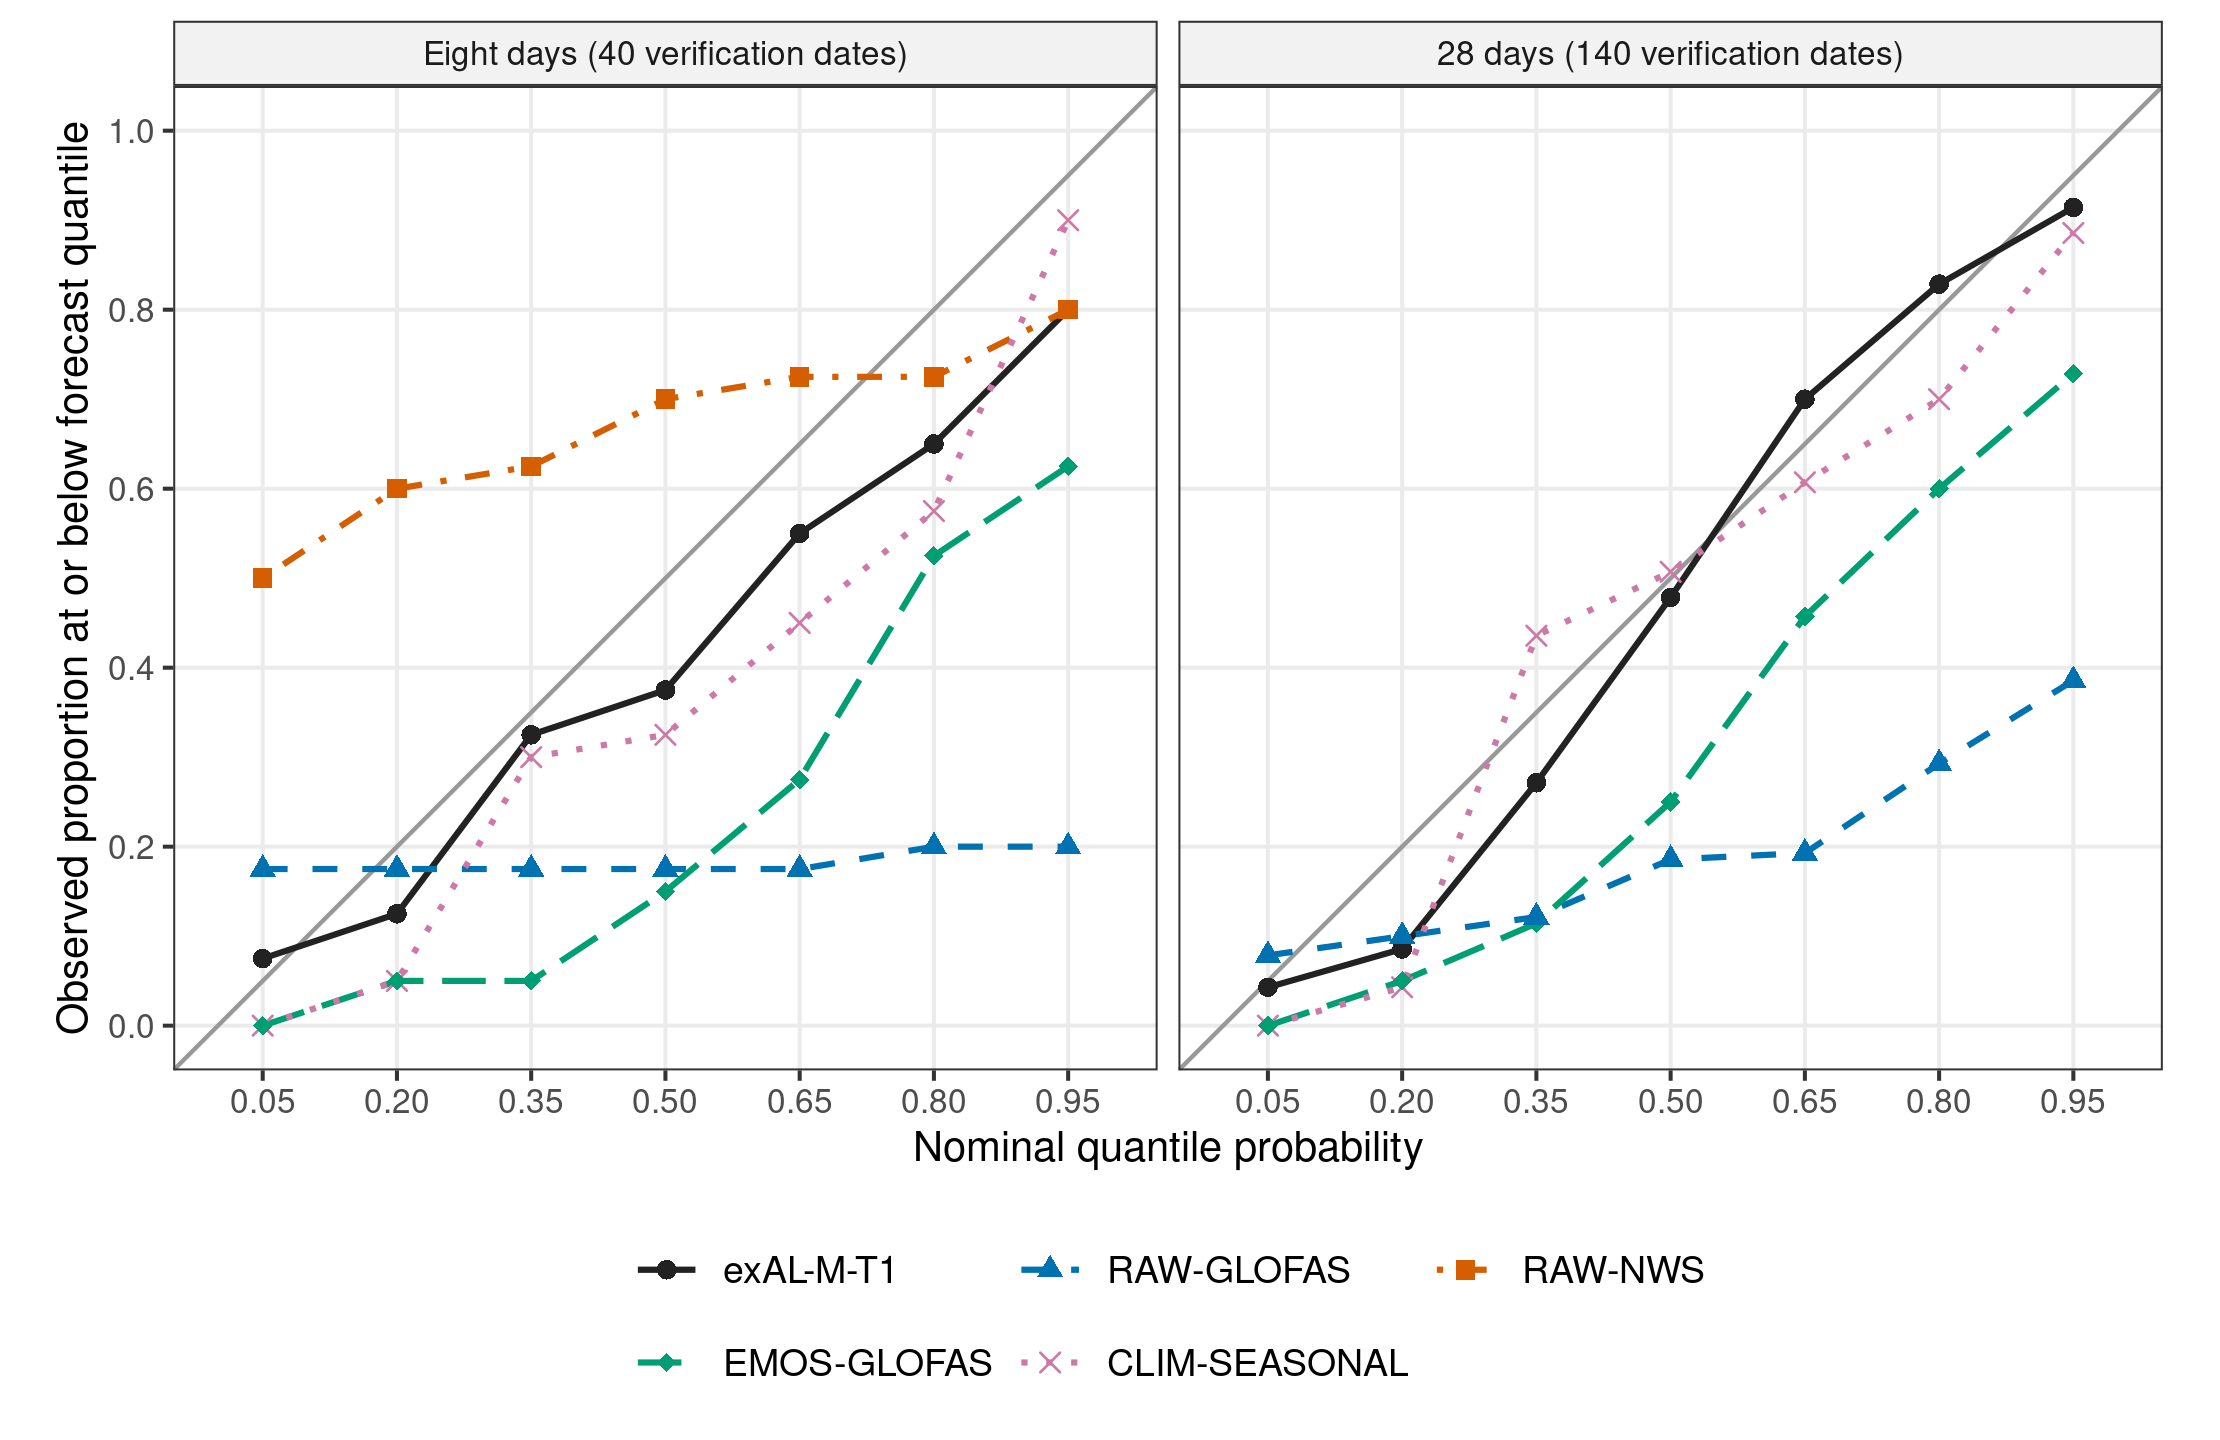
\includegraphics[width=450pt]{no_refit_quantile_reliability.png}
\caption{Empirical quantile reliability across the five forecast origins, separately for eight-day and 28-day horizons. Curves show the frequency of observations at or below each delivered predictive quantile for exAL-M-T1 and the raw-product, EMOS and seasonal references; the diagonal marks the nominal probability. Raw NWS is available over eight days. The companion records also retain strict frequencies and exact ties. These descriptive curves pool 40 and 140 cases, respectively.}
\label{fig:no_refit_reliability}
\end{figure}

The scoring scale also matters (Appendix Table~\ref{tab:no_refit_original_scale}). On the discharge scale, exAL-M-T1 has aggregate 28-day CRPS 6.26885~m$^3$/s and skill 0.39113. Over eight days, raw NWS has lower CRPS than exAL-M-T1, 6.63303 versus 7.49362~m$^3$/s, reversing their aggregate transformed-scale ranking. Very large discharge-scale scores for N-M-T1 and exAL-M-T0 reveal sensitivity to extreme predictive values. These findings limit a single scale-independent interpretation of the transformed-scale advantage.

\subsection{Component Sensitivity and Fitting Evidence}
\label{subsec:componentresults}

Appendix~\ref{app:he3ablation} reports a component-removal sensitivity analysis of the selected extended-likelihood multivariate model. Appendix Tables~\ref{tab:he3_ablation_crps} and \ref{tab:he3_ablation_crps_nws_horizon} give the corresponding 28-day and eight-day comparisons. Every reduced model has higher CRPS than both the full reference and raw GloFAS at every origin over both horizons. The size and consistency of these degradations require attention to fitting as well as to model structure. They establish sensitivity of the selected configuration under inherited settings; alone they do not show that each component is intrinsically necessary or that a separately optimized reduced model could not perform well.

The saved criteria show that 174 of the 175 reduced-model quantile fits reached their iteration budgets without established joint convergence; so did all 35 quantile fits of the full exAL-M-T1 reference. This limitation is therefore not specific to the poorly performing reductions. One striking reduced-fit case is the May 2022 transfer-free (\texttt{noTF}) model: its fitted median locations lie between 10.53 and 10.81 while transformed verification values lie between 0.42 and 0.57. Conversely, the Gaussian fits satisfy their recorded criteria despite some poor forecast scores. The audit thus identifies both fitting limitations and substantial predictive mismatch, but cannot assign every performance difference to a numerical cause. Appendix~\ref{app:fitdiagnostics} provides the complete classification and its limits.

\subsection{Supporting Interpretation}
\label{sec:interpretation}

The following summaries describe the reference exAL-M-T1 fit at December 25, 2022. Parameter intervals and historical latent-state bands describe approximate VB posterior uncertainty. The mean-field separation and local Laplace--Delta approximation can omit posterior dependence \citep{blei2017variational}; neither a narrow interval nor the predictive-coverage analysis establishes exact parameter-posterior calibration. Observation predictive intervals additionally include observation variation and the synthesis step.

Detailed source-specific summaries for the exAL shape and scale parameters are reported in Appendix~\ref{app:sourceparams}, with skewness and scale summaries in Appendix Tables~\ref{tab:gamma_sigma_intervals1} and \ref{tab:gamma_sigma_intervals2}. In the main text, we focus on the most interpretable features of the selected model.

\subsubsection{Covariate Effects}

\begin{table*}[htbp]
\centering
\begin{threeparttable}
\caption{Selected Posterior Means and 95\% Credible Intervals for Transfer-Function Covariates}
\label{tab:components_23_31}
\begin{tabular*}{\textwidth}{@{\extracolsep{\fill}} l c S[table-format=-1.5] l }
\toprule
\textbf{Covariate} & \textbf{Quantile} & \textbf{Mean} & \textbf{95\% CI} \\
\midrule
\multirow{3}{*}{Precipitation}  & 5th & -0.10282 & $[-0.10724,\ -0.09853]$ \\
& 50th & -0.06258 & $[-0.06830,\ -0.05698]$ \\
& 95th & 0.08632 & $[0.08044,\ 0.09208]$ \\
\midrule
\multirow{3}{*}{Soil Moisture}  & 5th & -0.02695 & $[-0.03315,\ -0.02082]$ \\
& 50th & -0.03325 & $[-0.04149,\ -0.02512]$ \\
& 95th & 0.01462 & $[0.00546,\ 0.02384]$ \\
\midrule
\multirow{3}{*}{First GDPC factor}  & 5th & -0.00198 & $[-0.00202,\ -0.00193]$ \\
& 50th & -0.00132 & $[-0.00137,\ -0.00126]$ \\
& 95th & -0.00116 & $[-0.00122,\ -0.00110]$ \\
\bottomrule
\end{tabular*}
\begin{tablenotes}
\item \textit{Note:} Posterior means and 95\% credible intervals $[{\rm Q2.5}, {\rm Q97.5}]$ for selected transfer-function coefficients at the representative December 25, 2022 cutoff, for the 5th, 50th, and 95th quantile models. \texttt{First GDPC factor} refers to the first generalized dynamic principal component introduced in Section~\ref{sec:data}.
\end{tablenotes}
\end{threeparttable}
\end{table*}


Table~\ref{tab:components_23_31} reports means and central 95\% intervals of the fitted variational marginals for three base-input transfer loadings at the 5th, 50th, and 95th quantiles. These are coefficient states \(\boldsymbol\psi_T\) at the terminal historical date, December 25, 2022, expressed per historical-standard-deviation unit of the corresponding input. They are not averages over the historical record. In the transition equation, \(\boldsymbol\psi_T\) contributes to the next transfer update through \(\mathbf x_{T+1}'\boldsymbol\psi_T\).

The coefficients describe conditional adjustments within a model that also contains source products, discrepancy states, seasonal structure, and nonlinear and lagged inputs. A negative linear precipitation loading does not imply that rainfall reduces total flow: the full feature vector and the autoregressive transfer state determine the adjustment. The isolated sign need not match an unconditional rainfall--flow relationship, and coefficient magnitudes do not measure physical importance across inputs. We interpret these quantities as dynamic transfer-feature loadings, without a causal interpretation. The companion feature dictionary identifies the complete state/feature layout.

\subsubsection{Historical Dynamics Across Representative Regimes}

To illustrate how the model behaves across contrasting hydrological conditions, we show posterior quantile dynamics for the exAL-M-T1 specification at the December 25, 2022 origin. The displayed windows cover the 2012--2016 drought and the 2017--2019 wet period. These figures are interpretation diagnostics: they show how the selected model decomposes fitted historical quantile behavior across contrasting regimes.

\begin{figure}[!htbp]
\centering
\includegraphics[width=450pt]{historical_summary_dry_period.png}
\caption{
Posterior mean and approximate 95\% VB credible intervals of river-flow quantiles during the dry period (2012--2016), estimated from the exAL-M-T1 model at the December 25, 2022 origin. Shown are the 5th (red), 50th (green), and 95th (blue) quantiles together with observed daily USGS flow (black). Horizontal dashed lines provide the lower and upper discharge references retained in this historical display.
}
\label{fig:dry_quantile}
\end{figure}

\begin{figure}[!htbp]
\centering
\includegraphics[width=450pt]{historical_summary_wet_period.png}
\caption{
Posterior mean and approximate 95\% VB credible intervals of river-flow quantiles during the wet period (2017--2019), estimated from the exAL-M-T1 model at the December 25, 2022 origin. Shown are the 5th (red), 50th (green), and 95th (blue) quantiles together with observed daily USGS flow (black). Horizontal dashed lines provide the lower and upper discharge references retained in this historical display.
}
\label{fig:rainy_quantile}
\end{figure}

Figures~\ref{fig:dry_quantile} and \ref{fig:rainy_quantile} compare the fitted posterior quantile dynamics during the drought and wet periods. During 2012--2016, the posterior bands remain comparatively narrow and the upper fitted quantile rarely approaches the current-rating NWS discharge-reference levels. During 2017--2019, winter peaks produce wider separation between the lower and upper fitted quantile curves, and the 95th quantile reaches levels comparable to the current-rating major-stage discharge reference in 2017 and 2019. This contrast indicates stronger upper-tail and cross-quantile variation during wetter regimes.

A complementary diagnostic is the long-cycle seasonal state. Figure~\ref{fig:80_components} shows this component alone for the same three representative quantile levels. The retained slow rotation has period 2474.87 days, approximately 6.78 calendar years or 81.3 months, as defined in Subsection~\ref{subsec:specification}. The component is broadly aligned across the three quantiles and varies over multi-year dry and wet phases in the historical record, illustrating how the selected state-space model separates long-cycle behavior from trend, transfer effects, and source-specific corrections.

\begin{figure}[!htbp]
\centering
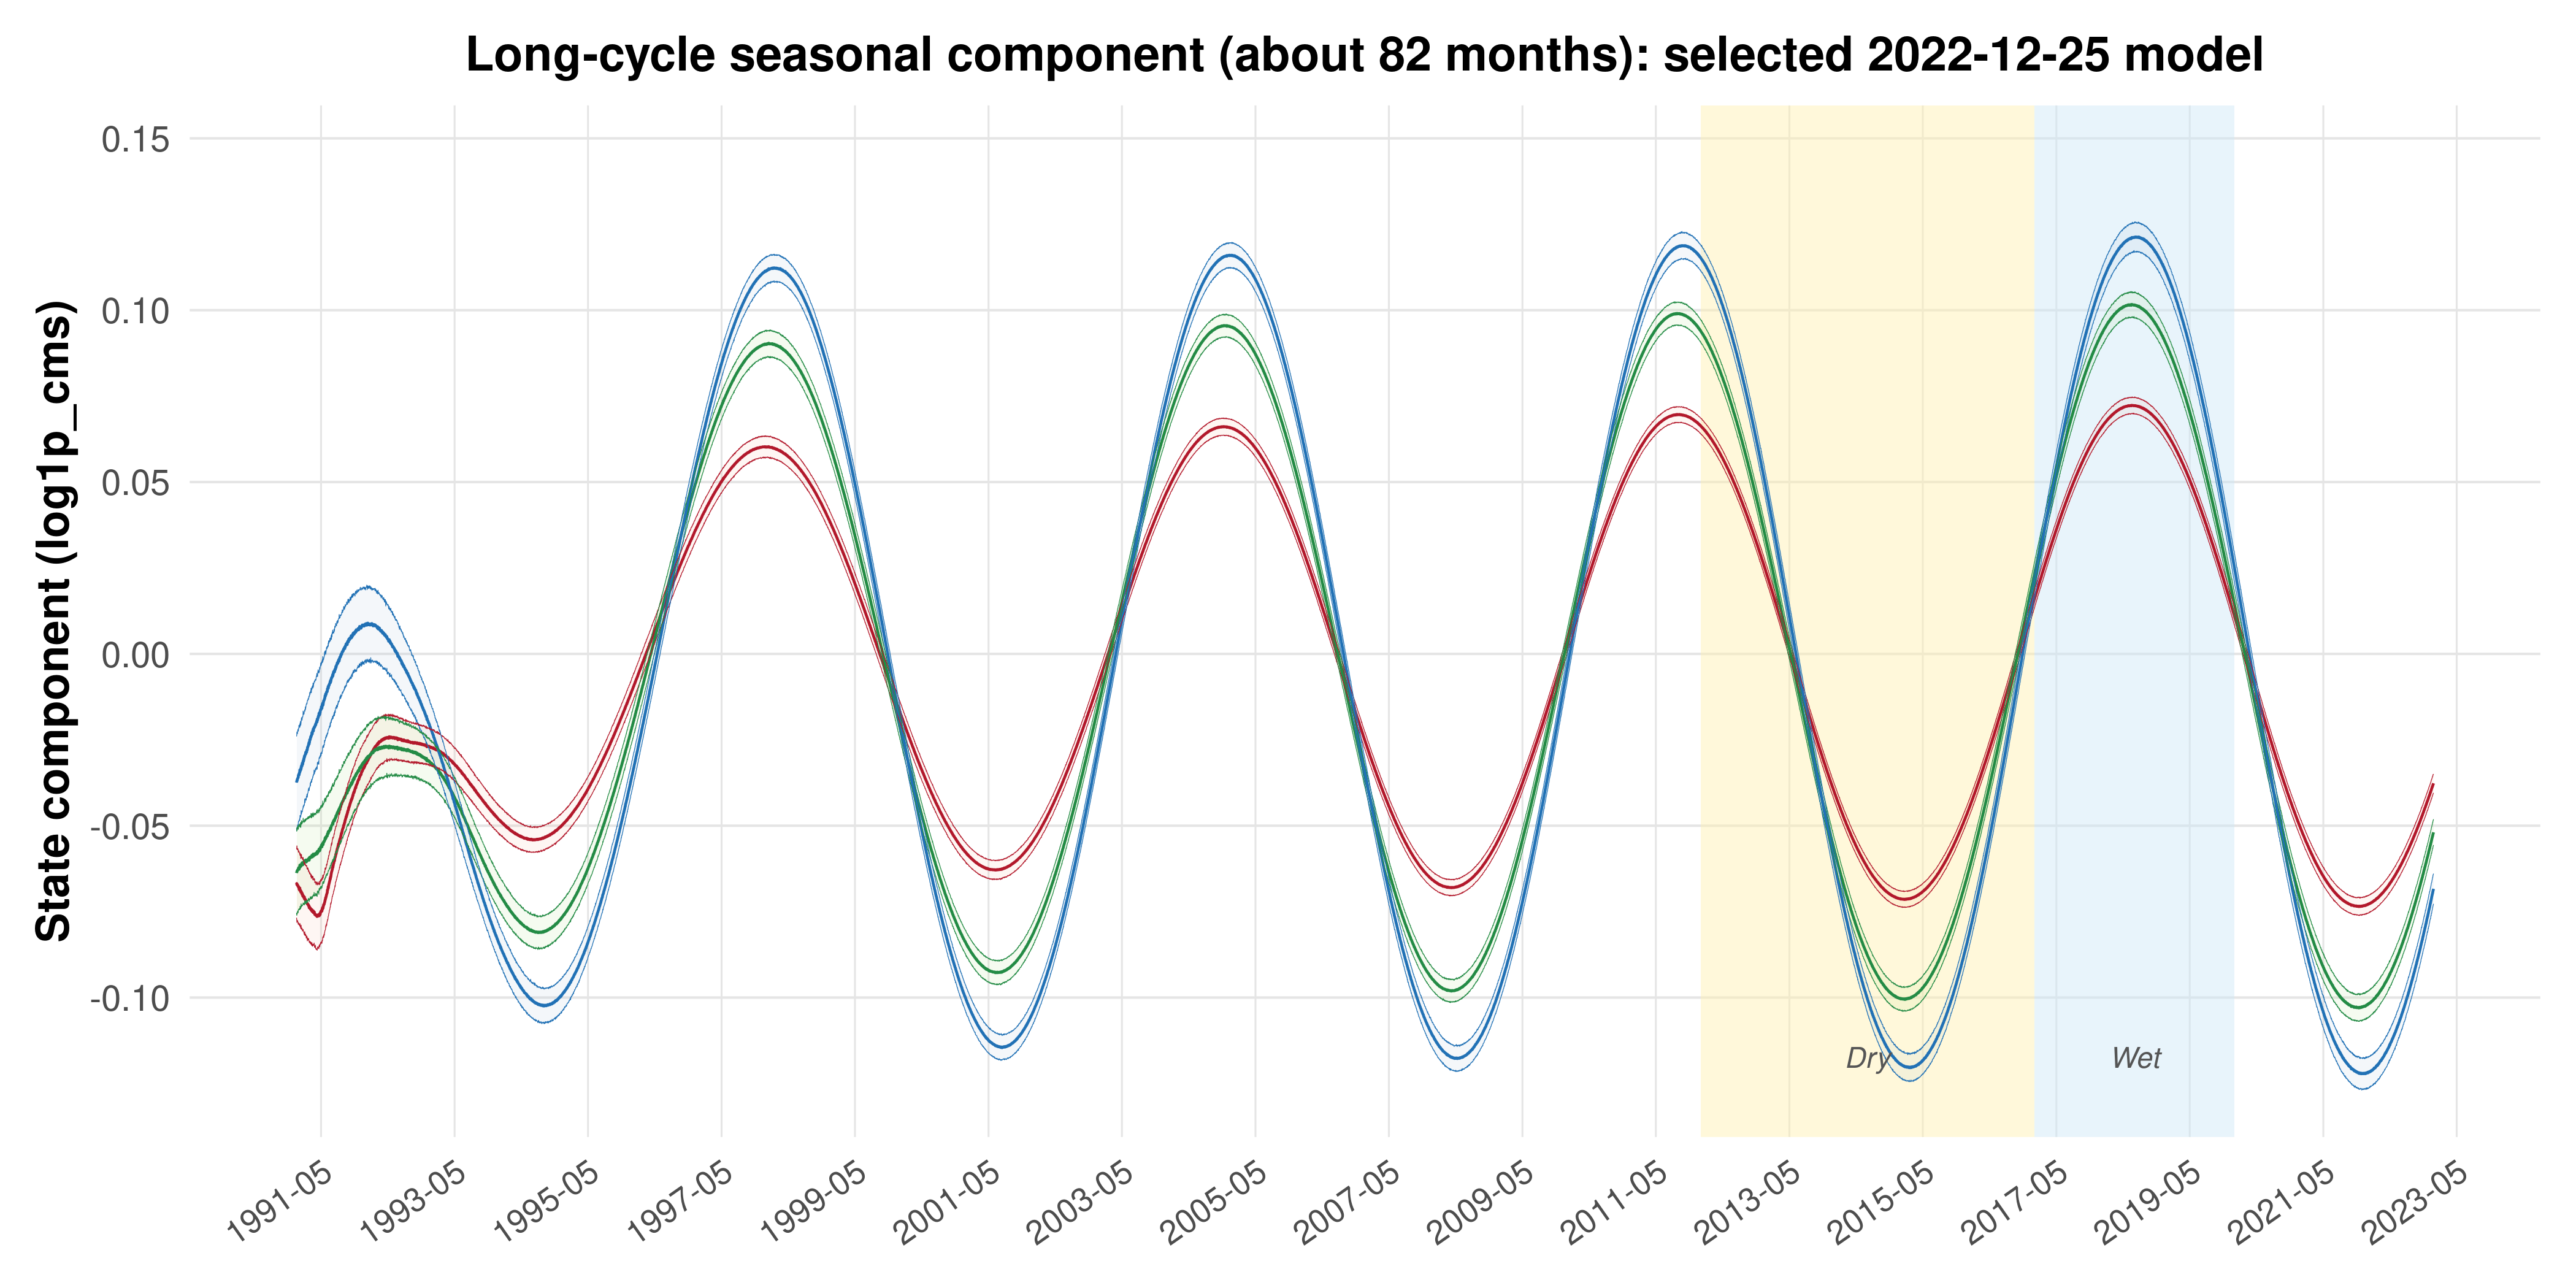
\includegraphics[width=450pt]{historical_component_80month.png}
\caption{
Selected-model posterior medians and approximate 95\% VB credible intervals for the long-cycle seasonal component, with period approximately 2474.87 days (6.78 calendar years), estimated from the exAL-M-T1 model at the December 25, 2022 origin. Estimates are shown for the 5th (red), 50th (green), and 95th (blue) quantiles. Shaded regions mark the 2012--2016 dry period and the 2017--2019 wet period.
}
\label{fig:80_components}
\end{figure}


\section{DISCUSSION AND CONCLUSIONS}
\label{sec5}

The proposed framework links gauge observations, retrospective products, and forecast ensembles through a dynamic quantile process with source-specific discrepancies. This supplies a common statistical representation while preserving the sources' different roles and horizons. A separate synthesis of the fitted quantile models produces the marginal predictive distributions used for forecast summaries and scoring. Laplace--Delta VB makes the extended-likelihood fits feasible for the multi-decade daily record.

In the San Lorenzo application, exAL-M-T1 has the lowest 28-day CRPS among the original framework variants and raw products at all five reported origins. Within those comparisons, raw NWS is strongest at two winter origins over eight days, while Bayesian variants are strongest at the other three. The added references show aggregate skill beyond seasonal climatology for the selected quantile models and for EMOS-GLOFAS, while the EMOS comparator outperforms exAL-M-T1 in May 2022. For a practitioner, these findings favor checking a single-product correction and simple references alongside the fuller source-and-covariate construction, at the horizon relevant to the decision. An aggregate advantage across five cases does not imply the best forecast at every origin or establish performance in another basin.

The Gaussian transfer comparison and the component-removal results also show why predictive scores should be read alongside fitting diagnostics. The full reference and nearly all reductions reach their iteration budgets without established joint convergence, so the ablations support conditional sensitivity conclusions. They do not establish the independent necessity of each component. Historical component summaries describe how the reference model allocates fitted variation; they are not independent evidence of forecast improvement.

The distribution checks further qualify the selected model's advantage. Its favorable mean transformed-scale score coexists with predictive undercoverage at the two December origins, and raw NWS has the better aggregate eight-day score on the discharge scale. Calibration, sharpness, forecast horizon and scoring scale address different practical aspects of prediction. The member-level likelihood additionally assumes conditional residual independence and a shared source scale across leads; the raw-product error and spread diagnostics retained with the article describe its inputs without validating those assumptions. Approximate VB parameter intervals remain distinct from predictive coverage, and their accuracy against full-model posterior simulation is an open computational assessment.

The framework depends on the external products, their alignment, and the supplied covariate paths. The five-origin evaluation samples contrasting conditions; a denser evaluation would require a larger version-consistent historical forecast archive. The present transfer inputs are deterministic summaries of uncertain hydrometeorological quantities. Future work could propagate their uncertainty jointly, fit dependent quantiles directly, enrich the discrepancy dynamics, and extend the model to multiple sites or basins.

\section*{Acknowledgments}

This work is part of the Ph.D. dissertation of Antonio De Leon in the statistical science program at the University of California, Santa Cruz.

\section*{Funding Statement}

This work was supported in part by the National Science Foundation under grant MMS2050012.

\section*{Conflict of Interest Statement}

The authors declare no conflict of interest.

\section*{Data Availability Statement}

The model-ready staged inputs, workflow code, manuscript-facing outputs, and provenance manifests for the quantile-model analysis are available in the public reproducibility repository \citep{deleon2026sanlorenzo_reproducibility}. The repository starts from curated staged inputs used by the reported analysis and does not bundle raw climate-center retrievals or intermediate covariate-preprocessing workflows. The underlying source products are public data products from USGS, ECMWF/GloFAS, NOAA/NWS, PRISM, ERA5-Land, GEFS, and NOAA Physical Sciences Laboratory, as described in the manuscript and repository. The external-reference inputs, code, results, and saved fitting evidence accompany the manuscript in the reproducibility bundle \texttt{artifacts/comment2\_revision}. The additional verification inputs, derived scores, calibration summaries, and reproduction code are supplied in \texttt{artifacts/no\_refit\_revision}.

\section*{Code availability}

The reusable estimation routines for the extended dynamic quantile linear model are available through the CRAN R package \texttt{exdqlm}, version 1.1.0 (\url{https://CRAN.R-project.org/package=exdqlm}; package DOI \url{https://doi.org/10.32614/CRAN.package.exdqlm}), and are described in \citet{deleon2026exdqlm}. The reproducibility repository cited in the Data Availability Statement contains the curated fitting and post-processing workflow code needed to reproduce the fits, validation summaries, tables, and figures of the quantile-model analysis from the staged inputs. Applying the workflow to a new basin requires staging the corresponding observations, current forecast products, and covariates. Reproducing the retrospective validation design additionally requires a basin-specific, version-consistent archive that aligns historical observations, retrospective products, issued forecast products, forecast-window covariates, product versions, spatial extraction rules, and source-specific forecast horizons.

\clearpage


\appendix
\renewcommand{\thefigure}{\Alph{section}\arabic{figure}}
\renewcommand{\thetable}{\Alph{section}\arabic{table}}


\section{Supplementary Parameter Summaries and Illustrations}
\label{app:extras}

\subsection{Component-Removal Sensitivity Analysis}
\label{app:he3ablation}

To assess how the selected specification depends on its main structural blocks, we refit \texttt{exAL-M-T1} after removing one component at a time. Each reduced model retains the reference forecast origins, input construction, likelihood, forecast horizons, and inherited scientific settings. The labels \texttt{noTrend}, \texttt{noH1}, \texttt{noH2}, and \texttt{noH3} remove, respectively, the local level or the first, second, or third seasonal pair from the shared and source-discrepancy structures. The third pair uses multiplier \(1/6.8068493\) and the 2474.87-day period defined in Subsection~\ref{subsec:specification}. The \texttt{noTF} configuration disables the covariate-transfer contribution in fitting and forecasting. It therefore differs from the main-table T0 comparison, which fits the historical transfer component and suppresses it only during the forecast window. These are fixed-policy structural sensitivity comparisons, not separate searches for each reduced model's best configuration.

\begin{table*}[htbp]
\centering
\renewcommand{\arraystretch}{1.08}
\begin{threeparttable}
\caption{Targeted 28-day ablation of the selected \texttt{exAL-M-T1} specification. Entries are mean forecast-window CRPS; lower values are better, and bold marks the best ablation-row value within each cutoff.}
\label{tab:he3_ablation_crps}
\begin{tabular*}{\textwidth}{@{\extracolsep{\fill}} >{\ttfamily}l r r r r r}
\toprule
Ablation model & 01/23/2021 & 11/12/2021 & 12/21/2021 & 05/11/2022 & 12/25/2022 \\
\midrule
exAL-M-T1 (full) & \textbf{0.13971} & \textbf{0.04724} & \textbf{0.26537} & \textbf{0.03233} & \textbf{0.66546} \\
exAL-M-T1-noTrend & 1.05159 & 0.72343 & 2.52043 & 0.55041 & 3.86618 \\
exAL-M-noTF & 1.73610 & 1.91285 & 1.79452 & 1.59694 & 2.36742 \\
exAL-M-T1-noH1 & 1.27861 & 1.60142 & 2.93841 & 1.15897 & 4.81220 \\
exAL-M-T1-noH2 & 0.72690 & 1.04724 & 2.93578 & 0.82020 & 4.45027 \\
exAL-M-T1-noH3 & 1.08281 & 1.03562 & 2.68667 & 0.72940 & 4.14478 \\
\addlinespace[2pt]
\multicolumn{6}{l}{\textit{Raw forecast products (reference only)}} \\
RAW-GLOFAS & 0.40366 & 0.16957 & 0.68246 & 0.27227 & 1.56006 \\
\bottomrule
\end{tabular*}
\begin{tablenotes}
\item \textit{Note:} Each ablation inherits the cutoff-specific winning \texttt{exAL-M-T1} input bundle, preprocessing, likelihood, and selected winner hyperparameters, changing only the named structural component. \texttt{RAW-GLOFAS} is shown as the 28-day raw reference; \texttt{RAW-NWS} is omitted because the archived NWS forecasts provide eight valid daily leads for these origins. \texttt{noH3} removes the third retained seasonal harmonic pair, where the third harmonic is the noninteger frequency \(1/6.8068493\).
\end{tablenotes}
\end{threeparttable}
\end{table*}


\begin{table*}[htbp]
\centering
\renewcommand{\arraystretch}{1.08}
\begin{threeparttable}
\caption{Targeted ablation CRPS over the common eight-day NWS forecast horizon. Lower values are better, and bold marks the best ablation-row value within each cutoff.}
\label{tab:he3_ablation_crps_nws_horizon}
\begin{tabular*}{\textwidth}{@{\extracolsep{\fill}} >{\ttfamily}l r r r r r}
\toprule
Ablation model & 01/23/2021 & 11/12/2021 & 12/21/2021 & 05/11/2022 & 12/25/2022 \\
\midrule
exAL-M-T1 (full) & \textbf{0.22691} & \textbf{0.05858} & \textbf{0.59445} & \textbf{0.02567} & \textbf{0.59070} \\
exAL-M-T1-noTrend & 1.49490 & 0.77464 & 3.38697 & 0.64627 & 3.40333 \\
exAL-M-noTF & 1.79777 & 1.69066 & 2.18697 & 2.45857 & 2.30863 \\
exAL-M-T1-noH1 & 1.66963 & 1.69424 & 3.70227 & 1.14270 & 3.79228 \\
exAL-M-T1-noH2 & 1.11122 & 1.14286 & 3.80753 & 0.99851 & 3.92807 \\
exAL-M-T1-noH3 & 1.53419 & 1.09181 & 3.45450 & 0.78219 & 3.75262 \\
\addlinespace[2pt]
\multicolumn{6}{l}{\textit{Raw forecast products (reference only)}} \\
RAW-GLOFAS & 0.57251 & 0.20670 & 1.29127 & 0.32274 & 1.48188 \\
RAW-NWS & 0.83037 & 1.37192 & 0.28118 & 0.28366 & 0.55680 \\
\bottomrule
\end{tabular*}
\begin{tablenotes}
\item \textit{Note:} This table restricts the full model, ablation variants, \texttt{RAW-GLOFAS}, and \texttt{RAW-NWS} to forecast leads 1--8, making it the horizon-compatible ablation reference for NWS.
\end{tablenotes}
\end{threeparttable}
\end{table*}


The full reference model has lower CRPS than each reduced model at all five origins over both horizons. All reduced-model scores also exceed the raw GloFAS reference. This is evidence that the selected configuration is sensitive to structural removal under its inherited fitting policy. Because removing a block changes the allocation of variation among the remaining states and can affect numerical estimation, the differences do not by themselves measure each block's independent forecast value. The sensitivity results support reporting the full configuration as fitted, with the fitting evidence and limitations considered explicitly.

\subsection{Saved Fitting Evidence}
\label{app:fitdiagnostics}

The audit covers 70 selected runs and 400 fits underlying the original configuration and component-removal comparisons. It reads the evaluated stopping criteria and terminal state recorded in the saved logs, together with iteration budgets, update counts, and sampling outcomes. Some historical routines print a convergence message unconditionally when their iteration loop ends. We do not count that message as evidence that their joint stopping conditions were satisfied. Likewise, zero parameter change during a frozen update is not evidence of convergence, and an inactive guard flag is not an actual sampling failure.

Table~\ref{tab:comment2_fit_diagnostics} summarizes the audit. Sixteen fits have evidence of satisfying their recorded criteria: 15 Gaussian dynamic linear model fits and the median fit for the January 2021 \texttt{noH1} reduction. Of the 315 multivariate quantile fits, the other 314 exhaust their recorded budgets without established joint convergence. This includes 174 of 175 component-removal fits and all 35 exAL-M-T1 reference fits. Three AL-M-T0 fits end with frozen updates, requiring particular caution in interpreting their terminal changes. The 70 univariate AL/exAL fits lack explicit joint-criterion records and are classified as unknown; this absence is not classified as failure.

% Generated by scripts/comment2_revision.py from checked frozen evidence.
\begin{table}[!htbp]
\centering
\begin{threeparttable}
\caption{Recorded stopping evidence for the existing benchmark and component-removal fits.}
\label{tab:comment2_fit_diagnostics}
\fontsize{8.5}{10.5}\selectfont
\begin{tabular}{lrrrrr}
\hline
Specification & Fits & Converged & Budget limit & Other & Unrecorded \\
\hline
AL-M-T0 & 35 & 0 & 35 & 0 & 0 \\
AL-M-T1 & 35 & 0 & 35 & 0 & 0 \\
AL-U-T1 & 35 & 0 & 0 & 0 & 35 \\
N-M-T0 & 5 & 5 & 0 & 0 & 0 \\
N-M-T1 & 5 & 5 & 0 & 0 & 0 \\
N-U-T1 & 5 & 5 & 0 & 0 & 0 \\
exAL-M-T0 & 35 & 0 & 35 & 0 & 0 \\
exAL-M-T1 & 35 & 0 & 35 & 0 & 0 \\
exAL-U-T1 & 35 & 0 & 0 & 0 & 35 \\
exAL-M-T1-noH1 & 35 & 1 & 34 & 0 & 0 \\
exAL-M-T1-noH2 & 35 & 0 & 35 & 0 & 0 \\
exAL-M-T1-noH3 & 35 & 0 & 35 & 0 & 0 \\
exAL-M-T1-noTrend & 35 & 0 & 35 & 0 & 0 \\
exAL-M-noTF & 35 & 0 & 35 & 0 & 0 \\
\hline
\end{tabular}
\begin{tablenotes}
\fontsize{8}{10}\selectfont
\item \textit{Note:} Counts refer to individual quantile fits, or one fit per Gaussian run. Converged means the saved criteria or explicit summary report convergence; it does not certify model validity. Budget limit means recorded criteria were unmet at the iteration limit. Other covers guards or criteria-unmet stops; unrecorded means sufficient stopping evidence is absent. Pipeline completion and a legacy terminal success phrase do not establish convergence.
\end{tablenotes}
\end{threeparttable}
\end{table}


These categories describe the available fitting evidence, not a test of forecast validity. In particular, completion and finite predictions do not establish convergence, whereas reaching an iteration limit does not by itself establish that a predictive distribution is unusable. The Gaussian criteria and the budget-limited full-reference fits show that the fitting categories do not separate good and poor forecast scores. Consequently, the tables document performance of the recorded fits, and the component-removal differences remain conditional sensitivities under the inherited settings. They do not resolve how independently retuned, more extensively converged reductions would perform.

\subsection{External References by Forecast Origin}
\label{app:externalreferences}

Table~\ref{tab:comment2_external_by_origin} gives the origin-specific scores and climatology-relative skill underlying the aggregate comparison. It retains the eight-day and 28-day horizons separately, so the seasonal reference and forecast methods are compared over identical verification dates within each block.

% Generated by scripts/comment2_revision.py from checked frozen evidence.
\begin{table}[!htbp]
\centering
\begin{threeparttable}
\caption{External-reference scores by forecast origin and horizon.}
\label{tab:comment2_external_by_origin}
\fontsize{8.5}{10.5}\selectfont
\begin{tabular}{lrrrrr}
\hline
Method & Jan 2021 & Nov 2021 & Dec 2021 & May 2022 & Dec 2022 \\
\hline
\multicolumn{6}{l}{\textit{28-day horizon}} \\
CLIM-SEASONAL & \shortstack[r]{0.45262\\(0.00000)} & \shortstack[r]{0.09588\\(0.00000)} & \shortstack[r]{0.79703\\(0.00000)} & \shortstack[r]{0.15235\\(0.00000)} & \shortstack[r]{1.71301\\(0.00000)} \\
PERSISTENCE & \shortstack[r]{0.62063\\(-0.37118)} & \shortstack[r]{0.22551\\(-1.35188)} & \shortstack[r]{0.69663\\(0.12597)} & \shortstack[r]{0.09059\\(0.40540)} & \shortstack[r]{2.91971\\(-0.70444)} \\
RAW-GLOFAS & \shortstack[r]{0.40366\\(0.10818)} & \shortstack[r]{0.16957\\(-0.76853)} & \shortstack[r]{0.68246\\(0.14374)} & \shortstack[r]{0.27227\\(-0.78715)} & \shortstack[r]{1.56006\\(0.08928)} \\
EMOS-GLOFAS & \shortstack[r]{0.26847\\(0.40686)} & \shortstack[r]{0.24060\\(-1.50931)} & \shortstack[r]{0.45633\\(0.42746)} & \shortstack[r]{0.01763\\(0.88427)} & \shortstack[r]{1.30369\\(0.23895)} \\
AL-M-T1 & \shortstack[r]{0.14592\\(0.67762)} & \shortstack[r]{0.05551\\(0.42107)} & \shortstack[r]{0.27775\\(0.65151)} & \shortstack[r]{0.05467\\(0.64112)} & \shortstack[r]{0.62764\\(0.63360)} \\
exAL-M-T1 & \shortstack[r]{0.13971\\(0.69134)} & \shortstack[r]{0.04724\\(0.50736)} & \shortstack[r]{0.26045\\(0.67323)} & \shortstack[r]{0.02273\\(0.85081)} & \shortstack[r]{0.53806\\(0.68590)} \\
\multicolumn{6}{l}{\textit{8-day horizon}} \\
CLIM-SEASONAL & \shortstack[r]{0.56808\\(0.00000)} & \shortstack[r]{0.06898\\(0.00000)} & \shortstack[r]{1.49136\\(0.00000)} & \shortstack[r]{0.16292\\(0.00000)} & \shortstack[r]{1.35522\\(0.00000)} \\
PERSISTENCE & \shortstack[r]{1.09161\\(-0.92159)} & \shortstack[r]{0.15108\\(-1.19020)} & \shortstack[r]{1.47804\\(0.00893)} & \shortstack[r]{0.03160\\(0.80603)} & \shortstack[r]{2.24035\\(-0.65312)} \\
RAW-GLOFAS & \shortstack[r]{0.57251\\(-0.00780)} & \shortstack[r]{0.20670\\(-1.99651)} & \shortstack[r]{1.29127\\(0.13417)} & \shortstack[r]{0.32274\\(-0.98098)} & \shortstack[r]{1.48188\\(-0.09346)} \\
RAW-NWS & \shortstack[r]{0.83037\\(-0.46171)} & \shortstack[r]{1.37192\\(-18.88862)} & \shortstack[r]{0.28118\\(0.81146)} & \shortstack[r]{0.28366\\(-0.74112)} & \shortstack[r]{0.55680\\(0.58914)} \\
EMOS-GLOFAS & \shortstack[r]{0.64070\\(-0.12784)} & \shortstack[r]{0.11361\\(-0.64706)} & \shortstack[r]{0.64016\\(0.57076)} & \shortstack[r]{0.02381\\(0.85384)} & \shortstack[r]{0.80423\\(0.40657)} \\
AL-M-T1 & \shortstack[r]{0.23740\\(0.58209)} & \shortstack[r]{0.07170\\(-0.03950)} & \shortstack[r]{0.56351\\(0.62215)} & \shortstack[r]{0.05867\\(0.63988)} & \shortstack[r]{0.61593\\(0.54552)} \\
exAL-M-T1 & \shortstack[r]{0.22691\\(0.60057)} & \shortstack[r]{0.05858\\(0.15078)} & \shortstack[r]{0.59445\\(0.60141)} & \shortstack[r]{0.02567\\(0.84242)} & \shortstack[r]{0.59070\\(0.56413)} \\
\hline
\end{tabular}
\begin{tablenotes}
\fontsize{8}{10}\selectfont
\item \textit{Note:} Each entry gives mean CRPS above climatology-relative CRPSS in parentheses. The exact origins are January 23, November 12 and December 21, 2021, and May 11 and December 25, 2022. Definitions match Table~\ref{tab:comment2_external_comparison}.
\end{tablenotes}
\end{threeparttable}
\end{table}


\subsection{Exact Settings and Additional Distribution Checks}
\label{app:distributionchecks}

Table~\ref{tab:no_refit_settings} reports the selected reference settings without rounding near-one discounts to unity. The accompanying records give all 45 benchmark configurations, including prior constants and implementation-resolved defaults. Table~\ref{tab:no_refit_sensitivity} separates empirical-distribution scores from the iid-based finite-sample sensitivity; Tables~\ref{tab:no_refit_original_scale} and \ref{tab:no_refit_origin_coverage} provide the discharge-scale comparison and predictive-coverage counts by origin. The reproducibility records additionally retain quantile hit counts and losses, predictive means and median errors, interval scores, and raw-source error/spread summaries by lead.

% Generated by scripts/no_refit_revision.py; do not edit.
\begin{table}[!htbp]
\centering
\begin{threeparttable}
\caption{Exact discount and initialization settings for the exAL-M-T1 reference fits.}
\label{tab:no_refit_settings}
\fontsize{8.5}{10.5}\selectfont
\setlength{\tabcolsep}{4pt}
\begin{tabular}{lrrrrrrr}
\hline
Origin & Trend & Annual & Slow & Discrepancy & Transfer & Loading & $\epsilon$ \\
\hline
Jan 2021 & $1-5\times 10^{-4}$ & $1-10^{-3}$ & $1-5\times 10^{-4}$ & $1-10^{-3}$ & $1-10^{-7}$ & $1-10^{-5}$ & $365$ \\
Nov 2021 & $1-5\times 10^{-4}$ & $1-10^{-3}$ & $1-5\times 10^{-4}$ & $1-10^{-3}$ & $1-10^{-7}$ & $1-10^{-5}$ & $365$ \\
Dec 2021 & $1-10^{-6}$ & $1-5\times 10^{-4}$ & $1-5\times 10^{-4}$ & $1-10^{-3}$ & $1-10^{-7}$ & $1-10^{-7}$ & $30$ \\
May 2022 & $1-10^{-7}$ & $1-5\times 10^{-4}$ & $1-5\times 10^{-4}$ & $1-10^{-3}$ & $1-10^{-6}$ & $1-10^{-6}$ & $1$ \\
Dec 2022 & $1-10^{-6}$ & $1-5\times 10^{-4}$ & $1-10^{-4}$ & $1-10^{-3}$ & $1-10^{-7}$ & $1-10^{-7}$ & $1$ \\
\hline
\end{tabular}
\begin{tablenotes}
\fontsize{8}{10}\selectfont
\item \textit{Note:} Both annual pairs have the annual discount shown. Discrepancy entries are multipliers applied to the corresponding trend/seasonal discounts. Transfer and loading columns refer to the autoregressive transfer state and feature-loading states. All rows use $\lambda=1-3\times10^{-2}$ and $c=1$. Exact settings, priors, resolved defaults and run identities for all 45 benchmark configurations are in the companion bundle.
\end{tablenotes}
\end{threeparttable}
\end{table}

% Generated by scripts/no_refit_revision.py; do not edit.
\begin{table}[!htbp]
\centering
\begin{threeparttable}
\caption{Finite-sample score sensitivity for all saved predictive representations.}
\label{tab:no_refit_sensitivity}
\fontsize{8.5}{10.5}\selectfont
\setlength{\tabcolsep}{4pt}
\begin{tabular}{lrrrr}
\hline
Method & 28-day ECDF & 28-day adjusted & 8-day ECDF & 8-day adjusted \\
\hline
N-U-T1 & 0.86656 & 0.86294 & 0.98660 & 0.98304 \\
N-M-T0 & 0.83341 & 0.82708 & 0.71763 & 0.71119 \\
N-M-T1 & 2.37057 & 2.35942 & 3.16734 & 3.15275 \\
AL-U-T1 & 0.60362 & 0.60358 & 0.34079 & 0.34072 \\
AL-M-T0 & 0.53804 & 0.53788 & 0.61352 & 0.61336 \\
AL-M-T1 & 0.23218 & 0.23206 & 0.30932 & 0.30920 \\
exAL-U-T1 & 0.59626 & 0.59621 & 0.35138 & 0.35132 \\
exAL-M-T0 & 1.13635 & 1.13511 & 1.13298 & 1.13174 \\
exAL-M-T1 & 0.20156 & 0.20149 & 0.29919 & 0.29912 \\
RAW-GLOFAS & 0.61456 & 0.61139 & 0.77322 & 0.77134 \\
RAW-NWS & --- & --- & 0.65025 & 0.63086 \\
CLIM-SEASONAL & 0.64197 & --- & 0.72911 & --- \\
PERSISTENCE & 0.91061 & --- & 0.99854 & --- \\
EMOS-GLOFAS & 0.45722 & --- & 0.44438 & --- \\
\hline
\end{tabular}
\begin{tablenotes}
\fontsize{8}{10}\selectfont
\item \textit{Note:} All scores use $\log(1+x)$. The adjusted pairwise score assumes independent, identically distributed draws from a predictive distribution. For physical members this is only a sensitivity assumption. Model sample counts are 2,000 for AL/exAL, 64 for N-U-T1 and 48 for N-M-T0/T1; raw GloFAS and NWS contain 51 and seven members. The adjustment is not applicable to deterministic climatology/EMOS grids or the persistence point mass. No adjusted skill score is reported.
\end{tablenotes}
\end{threeparttable}
\end{table}

% Generated by scripts/no_refit_revision.py; do not edit.
\begin{table}[!htbp]
\centering
\begin{threeparttable}
\caption{Distribution scores on the original discharge scale, in m$^3$/s.}
\label{tab:no_refit_original_scale}
\fontsize{8.5}{10.5}\selectfont
\setlength{\tabcolsep}{4pt}
\begin{tabular}{lrrrr}
\hline
Method & 28-day CRPS & 28-day CRPSS & 8-day CRPS & 8-day CRPSS \\
\hline
N-U-T1 & 11.92540 & -0.15827 & 12.37612 & -0.17558 \\
N-M-T0 & 10.95380 & -0.06390 & 9.97545 & 0.05245 \\
N-M-T1 & $2.03084\times 10^{9}$ & $-1.97248\times 10^{8}$ & $7.10790\times 10^{9}$ & $-6.75163\times 10^{8}$ \\
AL-U-T1 & 10.25614 & 0.00386 & 7.74218 & 0.26459 \\
AL-M-T0 & 10.13001 & 0.01611 & 10.42987 & 0.00929 \\
AL-M-T1 & 6.34032 & 0.38419 & 7.37167 & 0.29978 \\
exAL-U-T1 & 10.27183 & 0.00234 & 7.92688 & 0.24704 \\
exAL-M-T0 & 12307.63341 & -1194.39488 & 5460.23472 & -517.65541 \\
exAL-M-T1 & 6.26885 & 0.39113 & 7.49362 & 0.28820 \\
RAW-GLOFAS & 10.67159 & -0.03649 & 11.31853 & -0.07512 \\
RAW-NWS & --- & --- & 6.63303 & 0.36994 \\
CLIM-SEASONAL & 10.29587 & 0.00000 & 10.52767 & 0.00000 \\
PERSISTENCE & 11.98266 & -0.16383 & 12.37425 & -0.17540 \\
EMOS-GLOFAS & 9.59933 & 0.06765 & 9.03252 & 0.14202 \\
\hline
\end{tabular}
\begin{tablenotes}
\fontsize{8}{10}\selectfont
\item \textit{Note:} Each stored predictive value is inverse-transformed with $\exp(y)-1$ before scoring; transformed-scale scores are not exponentiated. Exact ECDF CRPS scores the equally weighted saved representation. CRPSS uses the frozen seasonal-climatology representation on the same cases and scale. Means pool 140 cases at 28 days and 40 cases at eight days. Raw NWS is available only through lead eight. The earlier tables retain the quantile-grid approximation.
\end{tablenotes}
\end{threeparttable}
\end{table}
% Generated by scripts/no_refit_revision.py; do not edit.
\begin{table}[!htbp]
\centering
\begin{threeparttable}
\caption{Predictive 95\% interval coverage by origin and horizon.}
\label{tab:no_refit_origin_coverage}
\fontsize{8.5}{10.5}\selectfont
\setlength{\tabcolsep}{4pt}
\begin{tabular}{lrrrrr}
\hline
Method & Jan 2021 & Nov 2021 & Dec 2021 & May 2022 & Dec 2022 \\
\hline
\multicolumn{6}{l}{\textit{28-day horizon}} \\
N-U-T1 & 26/28 & 28/28 & 12/28 & 28/28 & 3/28 \\
N-M-T0 & 3/28 & 6/28 & 17/28 & 1/28 & 24/28 \\
N-M-T1 & 0/28 & 0/28 & 0/28 & 0/28 & 2/28 \\
AL-U-T1 & 15/28 & 20/28 & 5/28 & 24/28 & 3/28 \\
AL-M-T0 & 25/28 & 28/28 & 17/28 & 28/28 & 3/28 \\
AL-M-T1 & 28/28 & 28/28 & 26/28 & 27/28 & 23/28 \\
exAL-U-T1 & 17/28 & 27/28 & 2/28 & 26/28 & 3/28 \\
exAL-M-T0 & 28/28 & 28/28 & 28/28 & 28/28 & 28/28 \\
exAL-M-T1 & 27/28 & 28/28 & 21/28 & 28/28 & 19/28 \\
RAW-GLOFAS & 20/28 & 12/28 & 16/28 & 0/28 & 0/28 \\
CLIM-SEASONAL & 28/28 & 28/28 & 28/28 & 28/28 & 20/28 \\
PERSISTENCE & 0/28 & 0/28 & 0/28 & 0/28 & 0/28 \\
EMOS-GLOFAS & 24/28 & 17/28 & 27/28 & 28/28 & 10/28 \\
\multicolumn{6}{l}{\textit{8-day horizon}} \\
N-U-T1 & 6/8 & 8/8 & 0/8 & 8/8 & 2/8 \\
N-M-T0 & 3/8 & 6/8 & 8/8 & 1/8 & 5/8 \\
N-M-T1 & 0/8 & 0/8 & 0/8 & 0/8 & 0/8 \\
AL-U-T1 & 7/8 & 2/8 & 4/8 & 8/8 & 3/8 \\
AL-M-T0 & 5/8 & 8/8 & 1/8 & 8/8 & 3/8 \\
AL-M-T1 & 8/8 & 8/8 & 6/8 & 7/8 & 6/8 \\
exAL-U-T1 & 7/8 & 8/8 & 1/8 & 8/8 & 3/8 \\
exAL-M-T0 & 8/8 & 8/8 & 8/8 & 8/8 & 8/8 \\
exAL-M-T1 & 8/8 & 8/8 & 1/8 & 8/8 & 4/8 \\
RAW-GLOFAS & 1/8 & 0/8 & 0/8 & 0/8 & 0/8 \\
RAW-NWS & 1/8 & 0/8 & 7/8 & 0/8 & 4/8 \\
CLIM-SEASONAL & 8/8 & 8/8 & 8/8 & 8/8 & 7/8 \\
PERSISTENCE & 0/8 & 0/8 & 0/8 & 0/8 & 0/8 \\
EMOS-GLOFAS & 5/8 & 1/8 & 7/8 & 8/8 & 6/8 \\
\hline
\end{tabular}
\begin{tablenotes}
\fontsize{8}{10}\selectfont
\item \textit{Note:} Entries give covered observations divided by available cases using the same limits and closed-interval rule as Table~\ref{tab:no_refit_calibration}. This descriptive check does not treat successive daily cases as independent replicates. Full per-origin distribution scores, targeted-quantile counts and interval scores accompany the article.
\end{tablenotes}
\end{threeparttable}
\end{table}


\subsection{Supplementary Source-Specific Shape and Scale Parameters}
\label{app:sourceparams}

\begin{table*}[htbp]
\centering
\begin{threeparttable}
\caption{Posterior Medians and 95\% Credible Intervals for the Source-Specific Weight Coefficients $\gamma_j(\tau)$ at the Representative December 25, 2022 Cutoff}
\label{tab:gamma_sigma_intervals1}
\begin{tabular*}{\textwidth}{@{\extracolsep{\fill}} l
 S[table-format=-1.5] l
 S[table-format=-1.5] l
 S[table-format=-1.5] l
@{}}
\toprule
 & \multicolumn{2}{c}{\textbf{USGS}} & \multicolumn{2}{c}{\textbf{GLOFAS}} & \multicolumn{2}{c}{\textbf{NWS}} \\
\cmidrule(lr){2-3}\cmidrule(lr){4-5}\cmidrule(lr){6-7}
\textbf{Quantile} & \textbf{Median} & \textbf{95\% CI} & \textbf{Median} & \textbf{95\% CI} & \textbf{Median} & \textbf{95\% CI} \\
\midrule
05th & 0.84518 & $[0.83064,\ 0.85881]$ & 0.97496 & $[0.96029,\ 0.98916]$ & 0.48124 & $[0.47043,\ 0.49255]$ \\
20th & 0.09424 & $[0.08194,\ 0.10702]$ & 0.33544 & $[0.32203,\ 0.34881]$ & -0.00668 & $[-0.00924,\ -0.00413]$ \\
35th & -0.02763 & $[-0.03298,\ -0.02234]$ & 0.16221 & $[0.15243,\ 0.17236]$ & -0.04280 & $[-0.04707,\ -0.03841]$ \\
50th & -0.13196 & $[-0.14005,\ -0.12322]$ & 0.06336 & $[0.05671,\ 0.07050]$ & -0.13248 & $[-0.13938,\ -0.12523]$ \\
65th & -0.31071 & $[-0.32244,\ -0.29846]$ & 0.01977 & $[0.01512,\ 0.02466]$ & -0.27078 & $[-0.28067,\ -0.26029]$ \\
80th & -0.68543 & $[-0.70270,\ -0.66835]$ & -0.05100 & $[-0.06204,\ -0.04053]$ & -0.49724 & $[-0.51116,\ -0.48282]$ \\
95th & -2.13801 & $[-2.16788,\ -2.10810]$ & -0.72784 & $[-0.73970,\ -0.71634]$ & -1.49200 & $[-1.51264,\ -1.47052]$ \\
\bottomrule
\end{tabular*}
\begin{tablenotes}
\item \textit{Note:} Posterior medians and 95\% credible intervals $[{\rm Q2.5}, {\rm Q97.5}]$ for the source-specific synthesis weights $\gamma_j(\tau)$ at the representative December 25, 2022 cutoff. The quantile labels 05th through 95th correspond to the seven fitted quantile models. These summaries are included as supplementary appendix support rather than as primary forecast-validation evidence.
\end{tablenotes}
\end{threeparttable}
\end{table*}


\begin{table*}[htbp]
\centering
\begin{threeparttable}
\caption{Posterior Medians and 95\% Credible Intervals for the Source-Specific Scale Parameters $\sigma_j(\tau)$ at the Representative December 25, 2022 Cutoff}
\label{tab:gamma_sigma_intervals2}
\begin{tabular*}{\textwidth}{@{\extracolsep{\fill}} l
 S[table-format=1.5] l
 S[table-format=1.5] l
 S[table-format=1.5] l
@{}}
\toprule
 & \multicolumn{2}{c}{\textbf{USGS}} & \multicolumn{2}{c}{\textbf{GLOFAS}} & \multicolumn{2}{c}{\textbf{NWS}} \\
\cmidrule(lr){2-3}\cmidrule(lr){4-5}\cmidrule(lr){6-7}
\textbf{Quantile} & \textbf{Median} & \textbf{95\% CI} & \textbf{Median} & \textbf{95\% CI} & \textbf{Median} & \textbf{95\% CI} \\
\midrule
05th & 0.02205 & $[0.02175,\ 0.02234]$ & 0.01396 & $[0.01378,\ 0.01414]$ & 0.01903 & $[0.01878,\ 0.01929]$ \\
20th & 0.04873 & $[0.04804,\ 0.04942]$ & 0.02538 & $[0.02505,\ 0.02571]$ & 0.04100 & $[0.04042,\ 0.04160]$ \\
35th & 0.06431 & $[0.06340,\ 0.06525]$ & 0.03093 & $[0.03053,\ 0.03134]$ & 0.05797 & $[0.05714,\ 0.05882]$ \\
50th & 0.07219 & $[0.07115,\ 0.07316]$ & 0.03294 & $[0.03251,\ 0.03339]$ & 0.06815 & $[0.06716,\ 0.06917]$ \\
65th & 0.06763 & $[0.06666,\ 0.06854]$ & 0.03668 & $[0.03620,\ 0.03717]$ & 0.06870 & $[0.06770,\ 0.06966]$ \\
80th & 0.05567 & $[0.05495,\ 0.05639]$ & 0.03567 & $[0.03522,\ 0.03617]$ & 0.05823 & $[0.05746,\ 0.05905]$ \\
95th & 0.03790 & $[0.03748,\ 0.03834]$ & 0.02053 & $[0.02026,\ 0.02078]$ & 0.03587 & $[0.03545,\ 0.03632]$ \\
\bottomrule
\end{tabular*}
\begin{tablenotes}
\item \textit{Note:} Posterior medians and 95\% credible intervals $[{\rm Q2.5}, {\rm Q97.5}]$ for the source-specific scale parameters $\sigma_j(\tau)$ at the representative December 25, 2022 cutoff. These summaries are included as supplementary appendix support rather than as primary forecast-validation evidence.
\end{tablenotes}
\end{threeparttable}
\end{table*}


Tables~\ref{tab:gamma_sigma_intervals1} and \ref{tab:gamma_sigma_intervals2} provide summaries of the source-specific skewness (\(\gamma\)) and scale (\(\sigma\)) parameters in the exAL observation model, reported for the December 25, 2022 origin. Centers are medians and the limits are central 95\% intervals of the fitted variational marginals. These are likelihood-parameter summaries, not synthesis weights; their approximate uncertainty has the scope described in Subsection~\ref{sec:interpretation}.

\subsection{Univariate Transfer-Active Predictive Synthesis}
\label{app:historicalsynth}

\begin{figure}[!htbp]
\centering
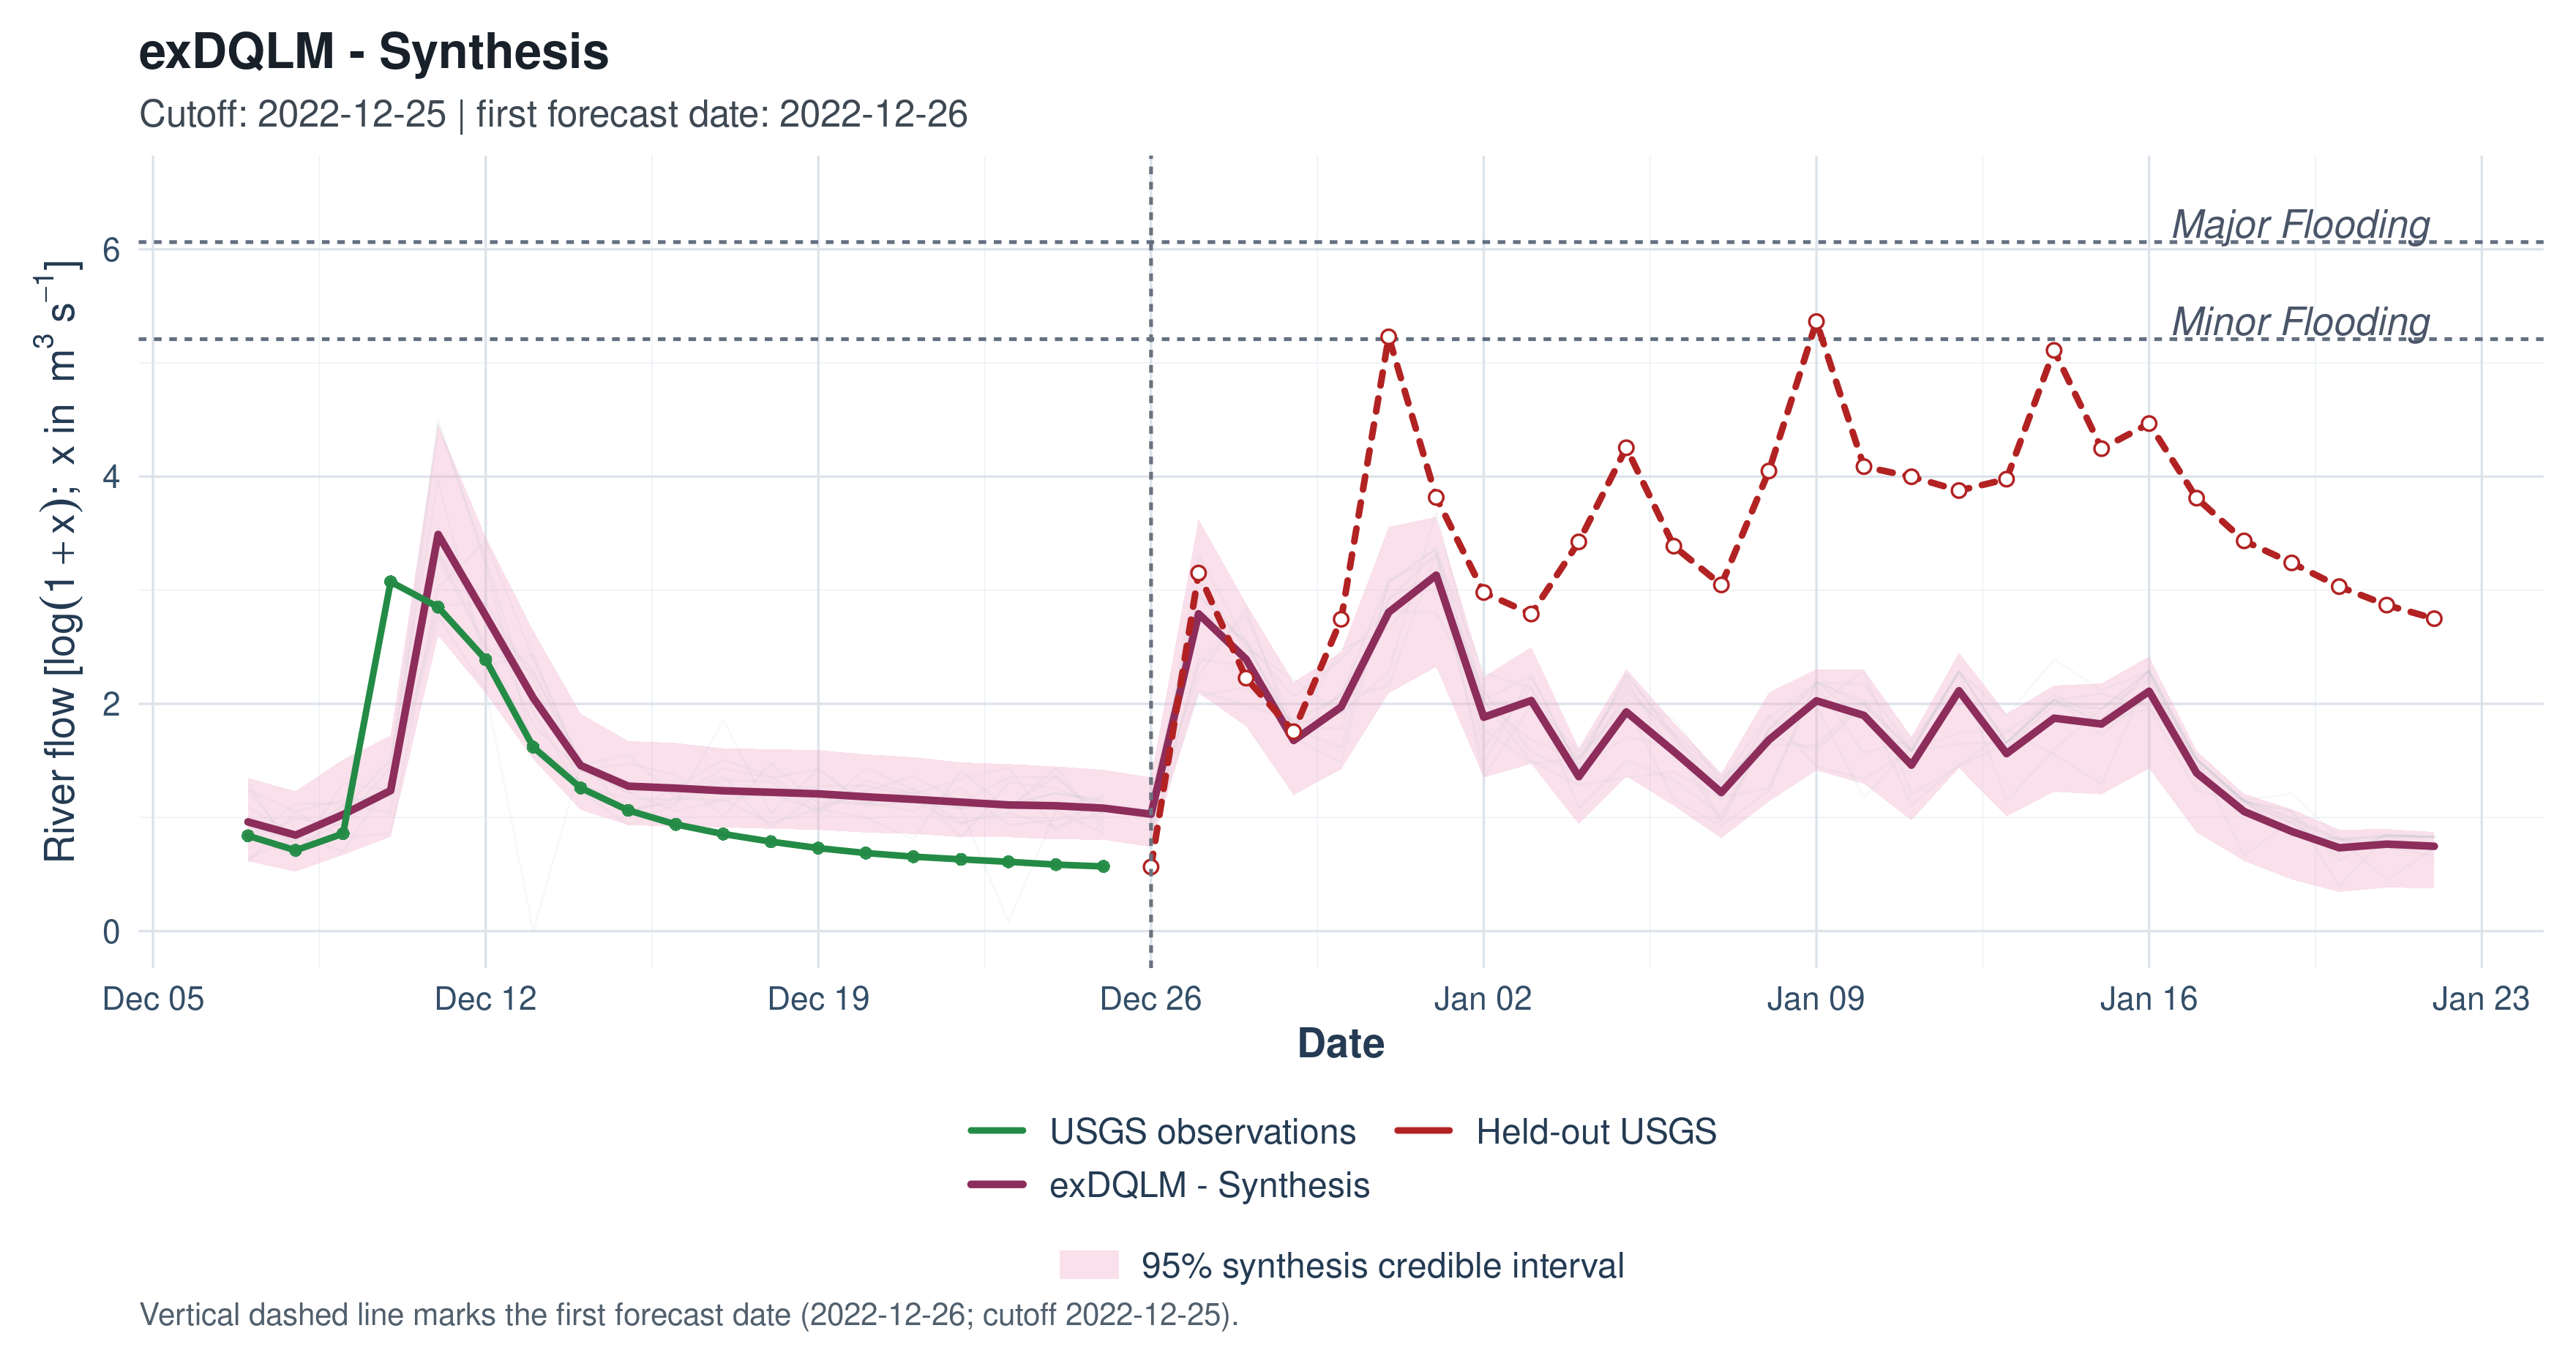
\includegraphics[width=450pt]{reference_synthesis_univariate.png}
\caption{
Univariate transfer-active predictive distribution for river flow on the $\log(1+x)$ scale, with $x$ measured in m$^3$/s, at the December 25, 2022 forecast origin. Observed measurements before the origin are shown in green, and held-out USGS verification after the origin is shown in red. The pink ribbon is the pointwise central 95\% predictive interval (2.5th--97.5th percentiles), and the dark line is the predictive mean on the \(\log(1+x)\) scale. The ten thin traces connect synthesized predictive sample values. The origin line marks \(T\), and the first forecast lead is \(T+1\). The reference uses the USGS observation channel and transfer covariates, and excludes the external source channels. Horizontal guides use the same discharge references as Figure~\ref{fig:synth1}.
}
\label{fig:synth2}
\end{figure}

Figure~\ref{fig:synth2} provides a univariate transfer-active reference for the December 25, 2022 origin. It is included to contrast the multivariate operational synthesis in Figure~\ref{fig:synth1} with a simpler reference that excludes retrospective-product and forecast-product source channels while retaining the transfer/covariate component.

\subsection{Additional Cutoff-Specific Predictive Synthesis Panels}
\label{app:cutoffsynthpanels}

The main text shows the December 25, 2022 synthesis as a representative selected-model illustration. For completeness, this appendix reports the corresponding multivariate synthesis panels for the other forecast origins. Each panel uses the same exAL-M-T1 synthesis specification as Figure~\ref{fig:synth1} and includes the retrospective and forecast-product references used at that cutoff.

\begin{figure}[p]
\centering
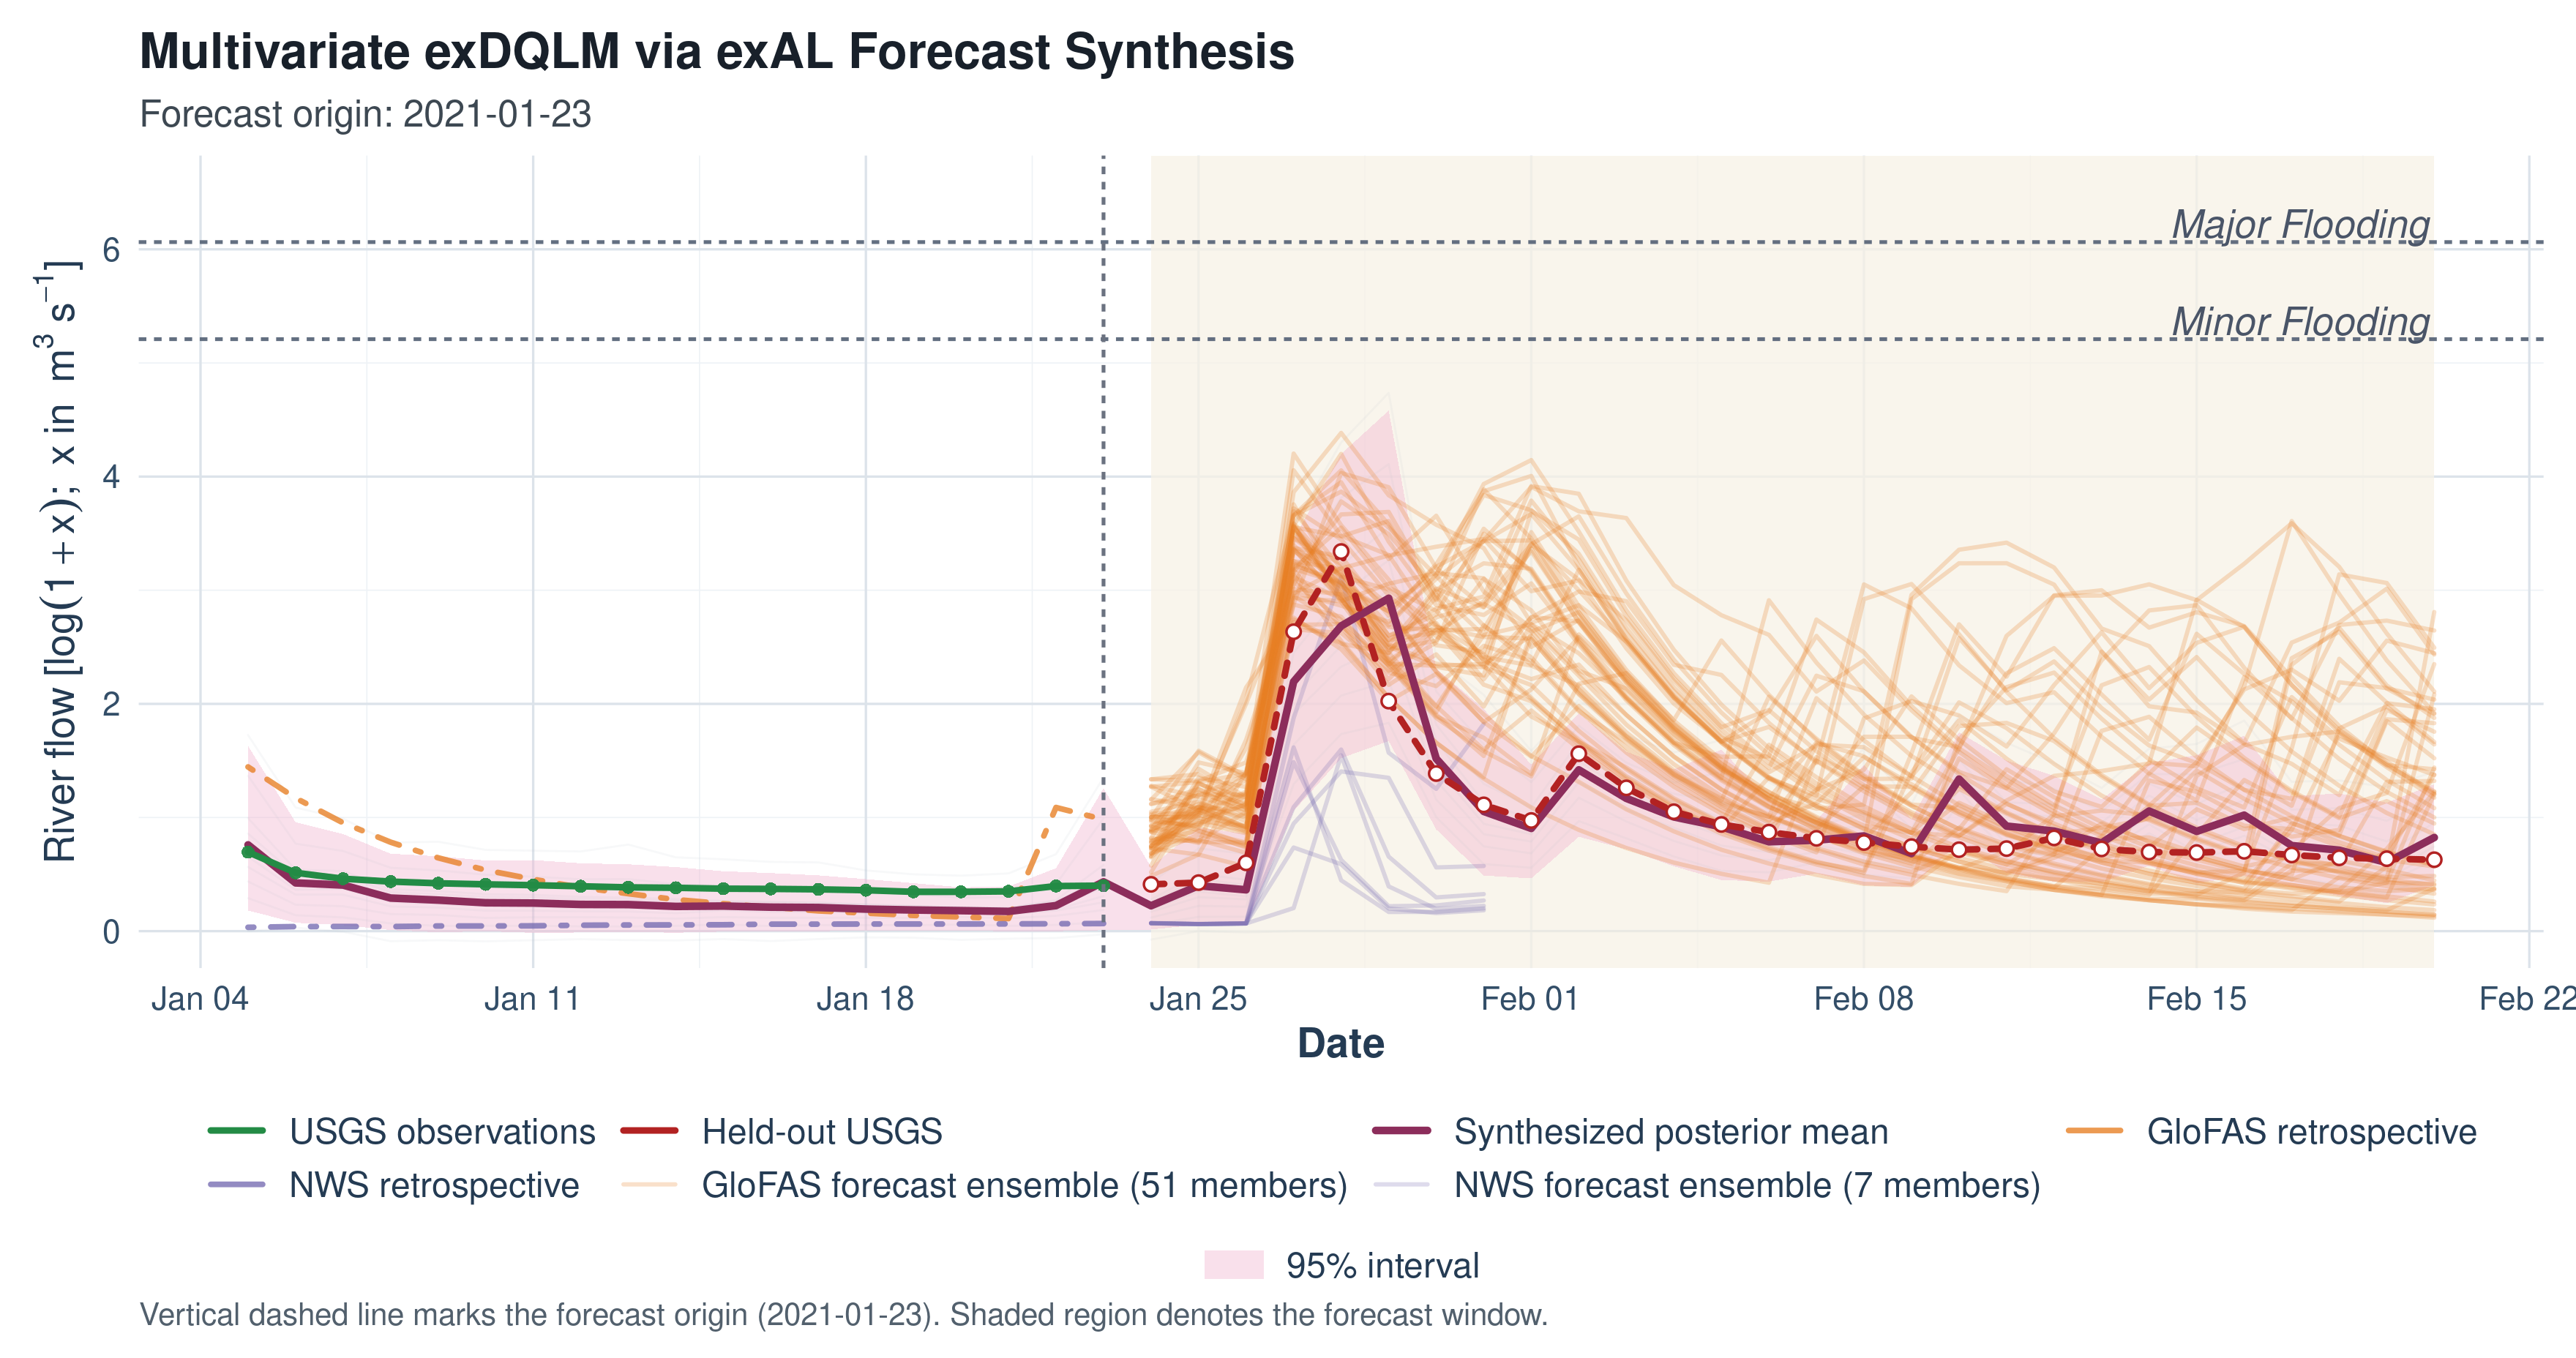
\includegraphics[width=450pt]{cutoff_2021_01_23_multivariate_synthesis_with_reference_ensembles.png}
\caption{
Predictive synthesis panel for the January 23, 2021 cutoff under the selected exAL-M-T1 specification. Observed USGS measurements before the origin are shown in green, and held-out USGS verification after the origin is shown in red. The pink ribbon is the pointwise central 95\% predictive interval (2.5th--97.5th percentiles), and the dark line is the predictive mean on the \(\log(1+x)\) scale. The ten thin traces connect synthesized predictive sample values. The origin line marks \(T\), and the first forecast lead is \(T+1\). Raw retrospective and forecast products are included as reference overlays. Horizontal guides use the same discharge references as Figure~\ref{fig:synth1}.
}
\label{fig:synthsupport_20210123}
\end{figure}

\begin{figure}[p]
\centering
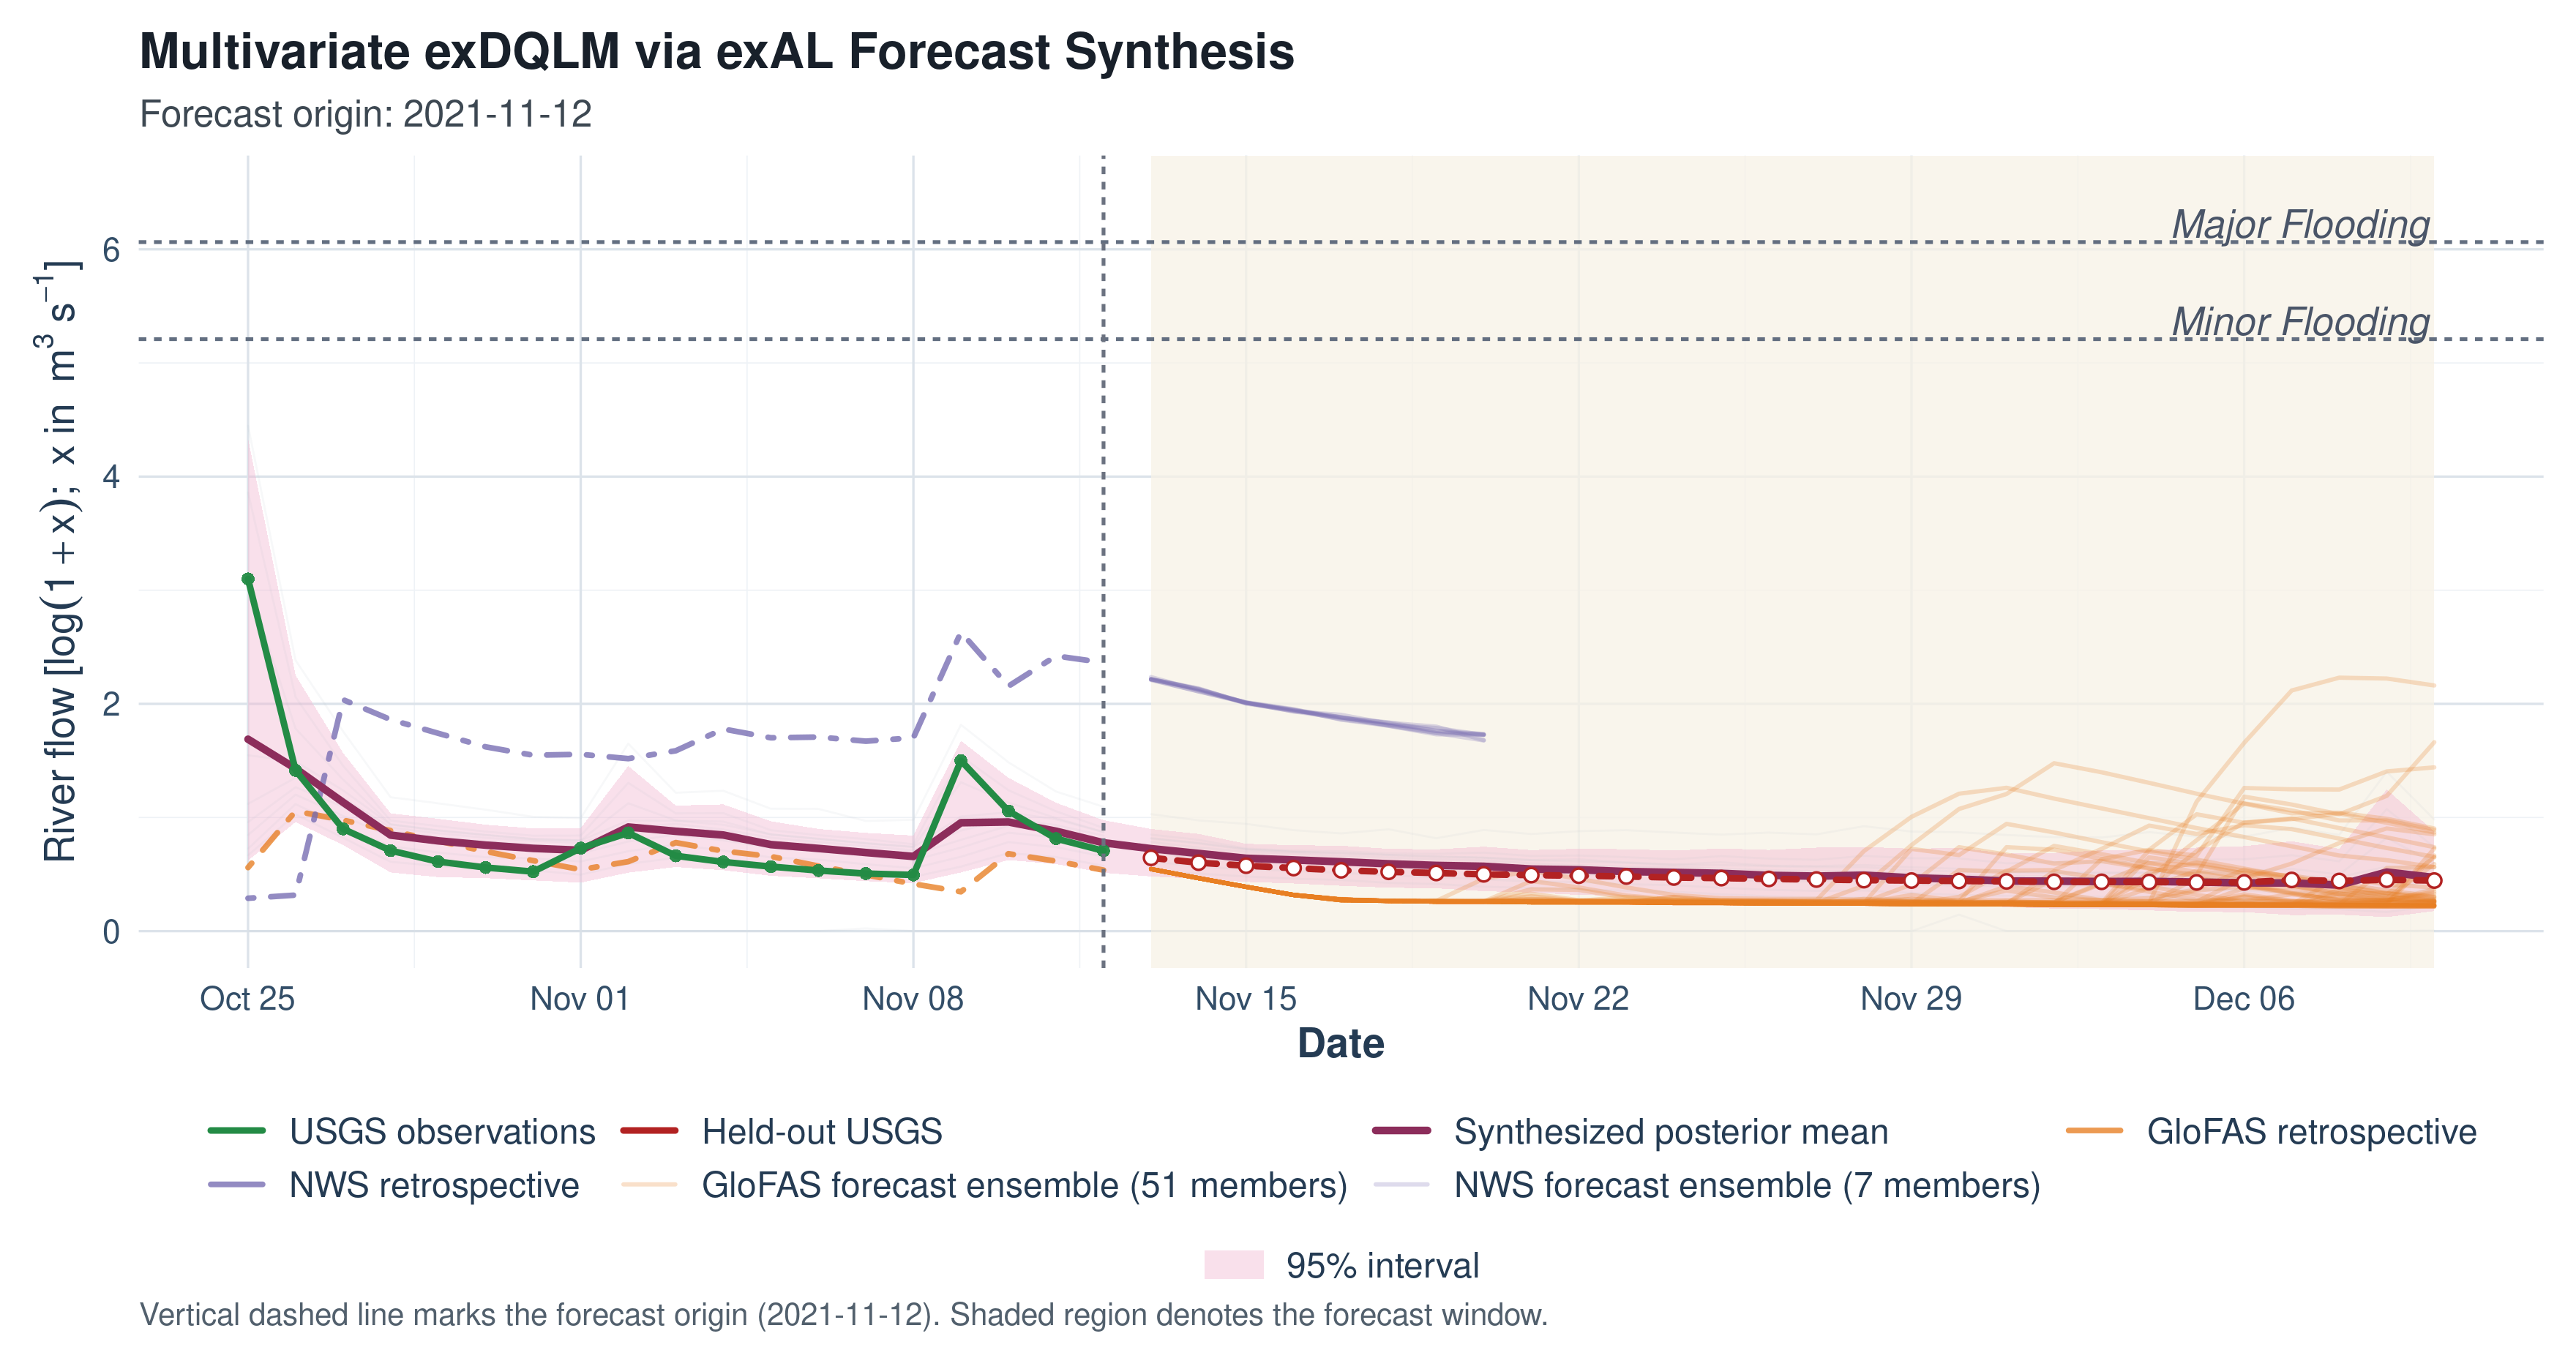
\includegraphics[width=450pt]{cutoff_2021_11_12_multivariate_synthesis_with_reference_ensembles.png}
\caption{
Predictive synthesis panel for the November 12, 2021 cutoff under the selected exAL-M-T1 specification. Observed USGS measurements before the origin are shown in green, and held-out USGS verification after the origin is shown in red. The pink ribbon is the pointwise central 95\% predictive interval (2.5th--97.5th percentiles), and the dark line is the predictive mean on the \(\log(1+x)\) scale. The ten thin traces connect synthesized predictive sample values. The origin line marks \(T\), and the first forecast lead is \(T+1\). Raw retrospective and forecast products are included as reference overlays. Horizontal guides use the same discharge references as Figure~\ref{fig:synth1}.
}
\label{fig:synthsupport_20211112}
\end{figure}

\begin{figure}[p]
\centering
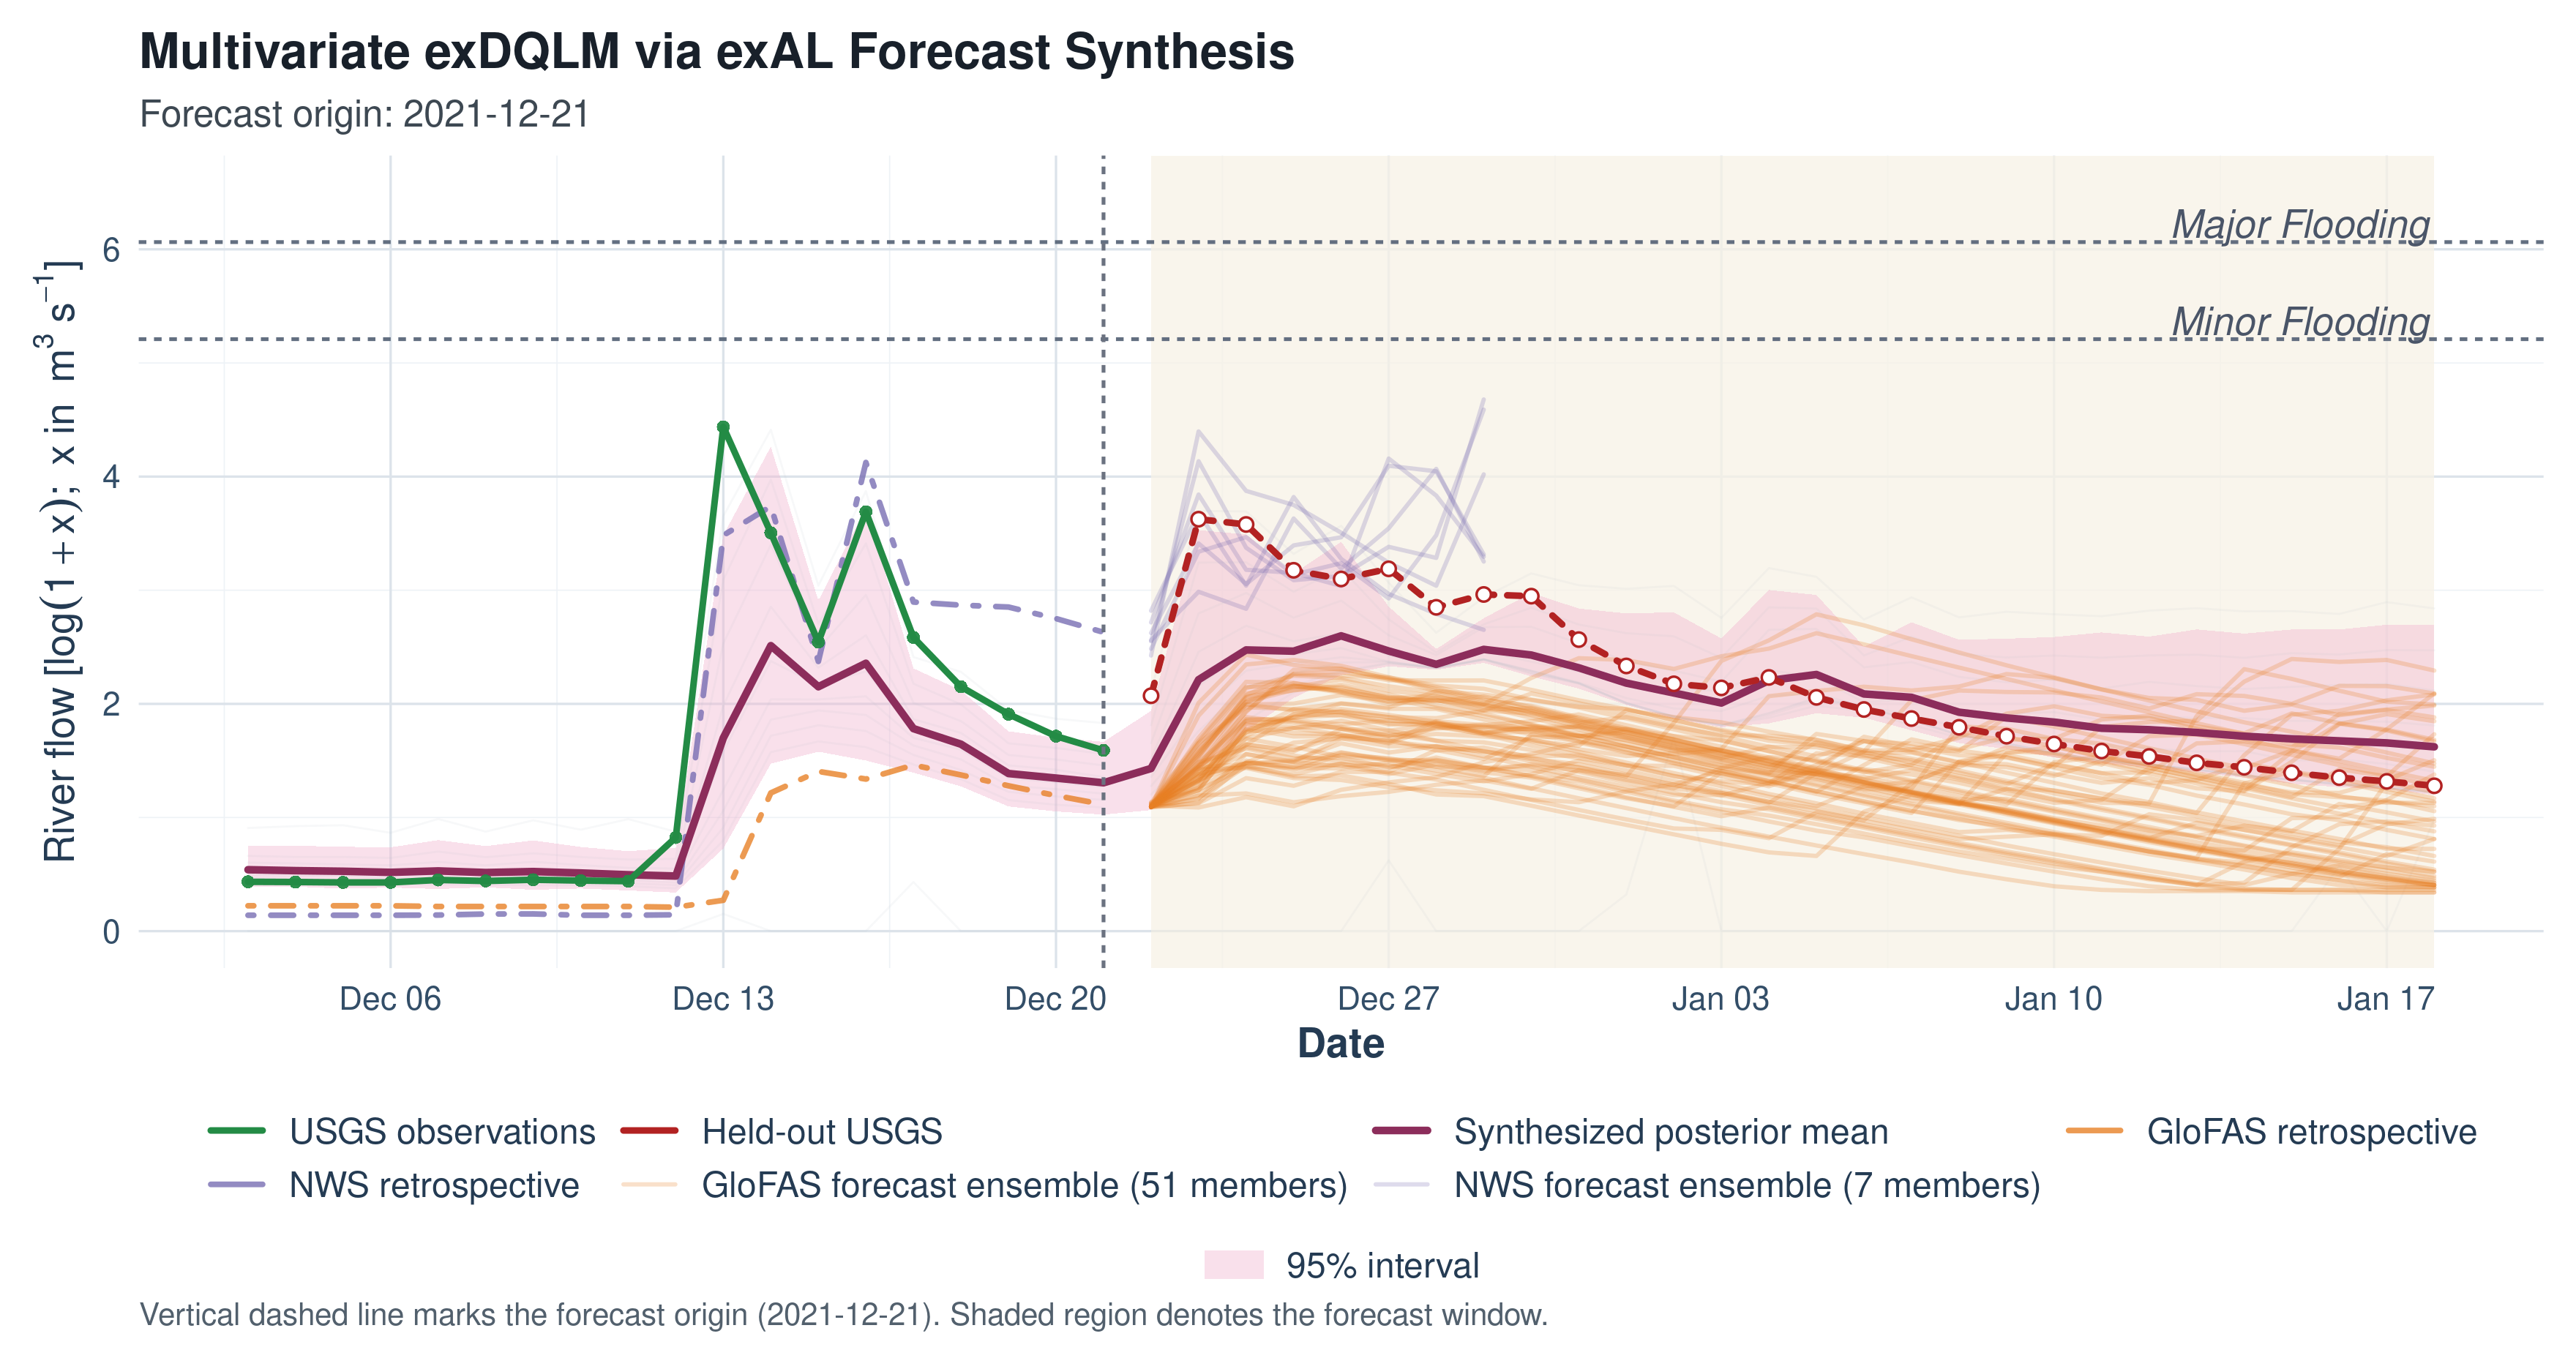
\includegraphics[width=450pt]{cutoff_2021_12_21_multivariate_synthesis_with_reference_ensembles.png}
\caption{
Predictive synthesis panel for the December 21, 2021 cutoff under the selected exAL-M-T1 specification. Observed USGS measurements before the origin are shown in green, and held-out USGS verification after the origin is shown in red. The pink ribbon is the pointwise central 95\% predictive interval (2.5th--97.5th percentiles), and the dark line is the predictive mean on the \(\log(1+x)\) scale. The ten thin traces connect synthesized predictive sample values. The origin line marks \(T\), and the first forecast lead is \(T+1\). Raw retrospective and forecast products are included as reference overlays. Horizontal guides use the same discharge references as Figure~\ref{fig:synth1}.
}
\label{fig:synthsupport_20211221}
\end{figure}

\begin{figure}[p]
\centering
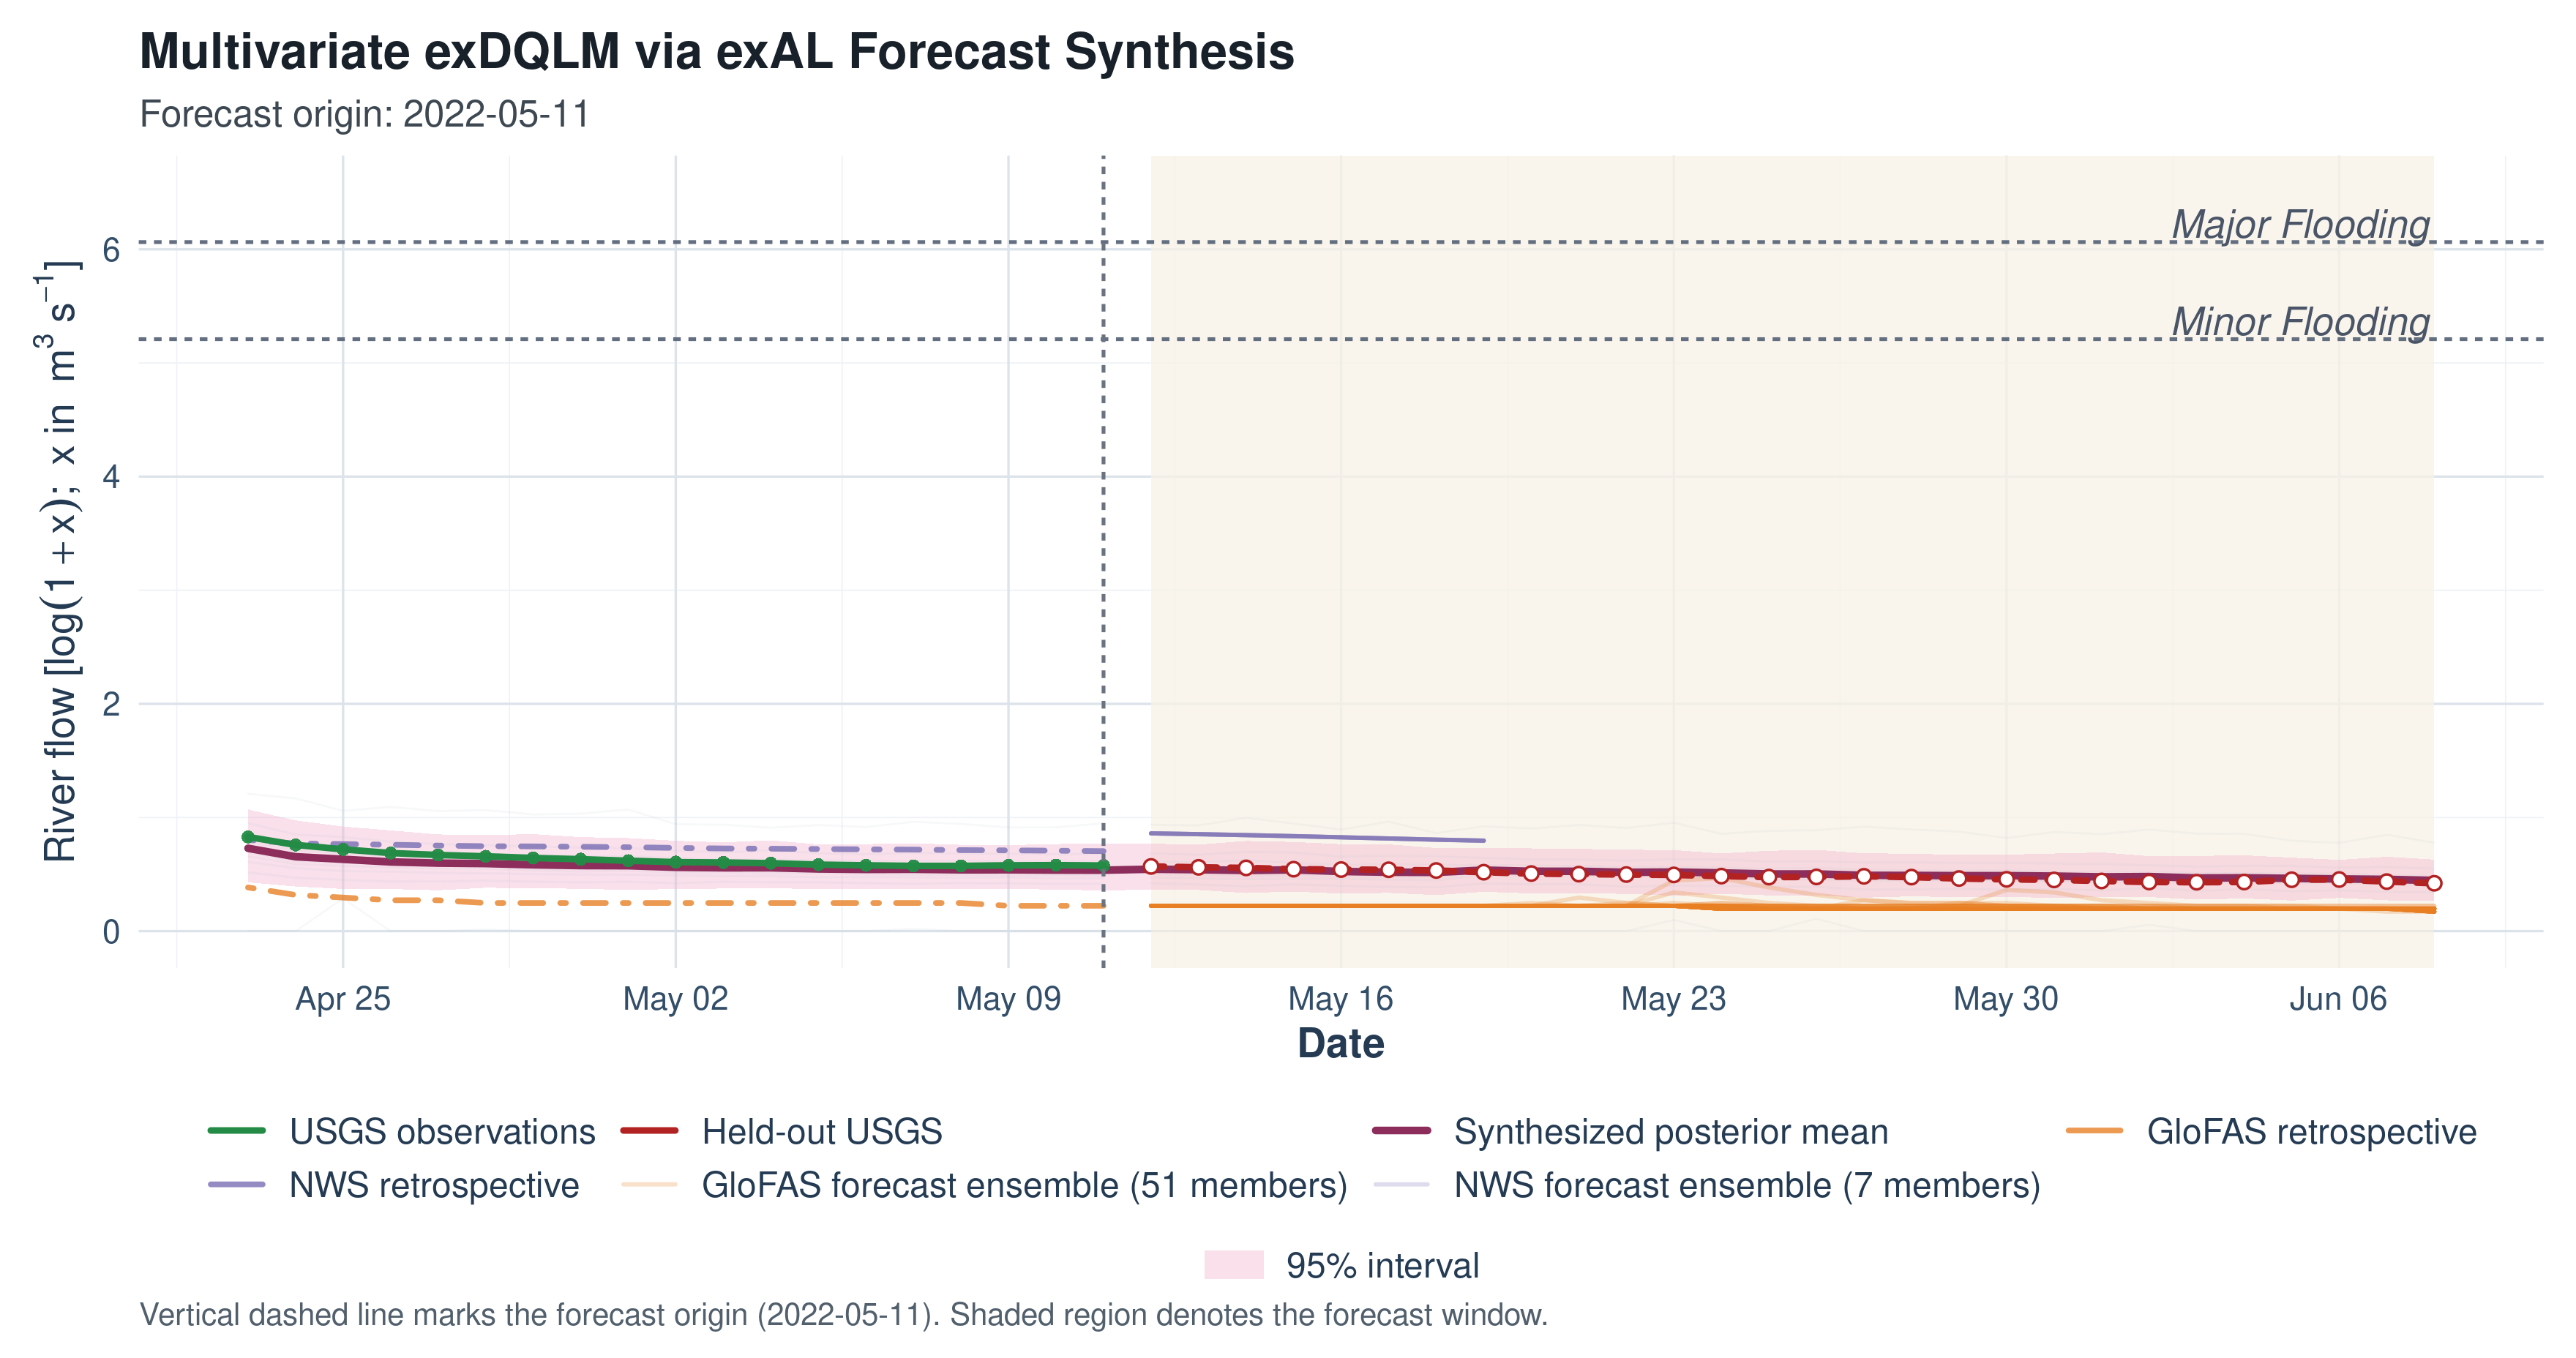
\includegraphics[width=450pt]{cutoff_2022_05_11_multivariate_synthesis_with_reference_ensembles.png}
\caption{
Predictive synthesis panel for the May 11, 2022 cutoff under the selected exAL-M-T1 specification. Observed USGS measurements before the origin are shown in green, and held-out USGS verification after the origin is shown in red. The pink ribbon is the pointwise central 95\% predictive interval (2.5th--97.5th percentiles), and the dark line is the predictive mean on the \(\log(1+x)\) scale. The ten thin traces connect synthesized predictive sample values. The origin line marks \(T\), and the first forecast lead is \(T+1\). Raw retrospective and forecast products are included as reference overlays. Horizontal guides use the same discharge references as Figure~\ref{fig:synth1}.
}
\label{fig:synthsupport_20220511}
\end{figure}

\section{State-Space Construction and Computational Details}
\label{app:stateconstruction}

\subsection{Stacked States and Selectors}

For the stacked state in Subsection~\ref{subsec:fullmodel}, define
\[
\boldsymbol{\omega}_t' = [\zeta_t,\ \boldsymbol{\psi}_t'], \qquad
\boldsymbol{\eta}_t' = [\boldsymbol{\theta}_t',\ (\boldsymbol{\delta}_t^1)',\ \ldots,\ (\boldsymbol{\delta}_t^J)',\ \boldsymbol{\omega}_t'],
\]
where \(\boldsymbol{\omega}_t \in \mathbb{R}^{m+1}\) and \(\boldsymbol{\eta}_t \in \mathbb{R}^{q}\), with \(q = (J+1)p + m + 1\). The transfer update can be written as
\[
\mathbf{G}^{\text{trans}}_t =
\begin{bmatrix}
\lambda & \mathbf{x}_t' \\
\mathbf{0}_m & \mathbf{I}_m
\end{bmatrix}.
\]
Let \(\mathcal{J}_0=\{0\}\cup\mathcal{J}\), where \(s=0\) denotes the USGS observation channel and \(s\in\mathcal{J}\) denotes an external product family. Let \(y_t^0 \equiv y_t^o\) denote the observation channel and \(y_t^s \equiv z_t^s\), \(s\in\mathcal{J}\), denote the retrospective-product channels. The corresponding compact form is:
\begin{alignat}{3}
\text{Pre-cutoff observations:}\quad&
y_t^s \mid \boldsymbol{\eta}_t, \sigma^s, \gamma^s
&\sim{}& \text{exAL}_{p_0}\!\left(\mathbf{h}_{t,s}' \boldsymbol{\eta}_t, \sigma^s, \gamma^s\right),
&\qquad& 1 \le t \le T,\ s \in \mathcal{J}_0, \label{eq:compact_est_obs}
\\
\text{Pre-cutoff state evolution:}\quad&
\boldsymbol{\eta}_t \mid \boldsymbol{\eta}_{t-1}
&\sim{}& \mathcal{N}\!\left(\boldsymbol{D}_t \boldsymbol{\eta}_{t-1}, \boldsymbol{\Lambda}_t\right),
&\qquad& 1 \le t \le T, \label{eq:compact_est_state}
\\
\text{Forecast observations:}\quad&
y_T^{j,i}(k) \mid \boldsymbol{\eta}_{T+k}, \sigma^j, \gamma^j
&\sim{}& \text{exAL}_{p_0}\!\left(\mathbf{e}_{T+k,j}' \boldsymbol{\eta}_{T+k}, \sigma^j, \gamma^j\right),
&\qquad& j \in \mathcal{J},\ i \in \mathcal{I}_j,\ k \in \mathcal{K}_j, \label{eq:compact_fc_obs}
\\
\text{Forecast state evolution:}\quad&
\boldsymbol{\eta}_{T+k} \mid \boldsymbol{\eta}_{T+k-1}
&\sim{}& \mathcal{N}\!\left(\boldsymbol{M}_{T+k} \boldsymbol{\eta}_{T+k-1}, \mathbf{W}_{T+k}\right),
&\qquad& 1 \le k \le K_{\max}. \label{eq:compact_fc_state}
\end{alignat}

Here
\[
\big(\mathbf{F}_t^{\text{trans}}\big)' = [1,\ \mathbf{0}_m'], \qquad
\mathbf{h}_{t,0}' =
\big[\mathbf{F}_t',\ \mathbf{0}_{pJ}',\ \big(\mathbf{F}_t^{\text{trans}}\big)'\big],
\qquad
\mathbf{h}_{t,j}' =
\big[\mathbf{F}_t',\ \mathbf{0}_{p(j-1)}',\ \mathbf{F}_t',\ \mathbf{0}_{p(J-j)}',\ \big(\mathbf{F}_t^{\text{trans}}\big)'\big],
\quad j \in \mathcal{J},
\]
with \(\mathbf{F}_t^{\text{trans}} \in \mathbb{R}^{m+1}\), \(\mathbf{h}_{t,0}, \mathbf{h}_{t,j} \in \mathbb{R}^{q}\), and
\[
\boldsymbol{D}_t = \text{BlockDiag}\!\left(\mathbf{G}_t,\ \underbrace{\mathbf{G}_t,\ldots,\mathbf{G}_t}_{J\ \text{discrepancy blocks}},\ \mathbf{G}^{\text{trans}}_t\right), \qquad
\boldsymbol{\Lambda}_t = \text{BlockDiag}\!\left(\mathbf{W}^{\theta}_t,\ \underbrace{\mathbf{W}^{\delta^1}_t,\ldots,\mathbf{W}^{\delta^J}_t}_{J\ \text{source-specific discrepancy blocks}},\ \text{BlockDiag}\!\left(w_t^{\zeta}, \mathbf{W}^{\psi}_t\right)\right),
\]
where \(\boldsymbol{D}_t, \boldsymbol{\Lambda}_t \in \mathbb{R}^{q\times q}\) and \(\sigma^s \in \mathbb{R}_+\), \(\gamma^s \in \mathbb{R}\) denote the channel-specific scale and skewness parameters for \(s \in \mathcal{J}_0\). Thus, \(\mathbf{h}_{t,0}' \boldsymbol{\eta}_t = \mathbf{F}_t' \boldsymbol{\theta}_t + \zeta_t\) and \(\mathbf{h}_{t,j}' \boldsymbol{\eta}_t = \mathbf{F}_t'(\boldsymbol{\theta}_t + \boldsymbol{\delta}_t^j) + \zeta_t\). For the forecast window, \(\mathbf{e}_{T+k,j}\) is the analogue of \(\mathbf{h}_{t,j}\): it extracts the latent trend-and-seasonal block, the discrepancy block for source \(j\), and the transfer block. The matrices \(\boldsymbol{M}_{T+k}\) and \(\mathbf{W}_{T+k}\) preserve the same block ordering while propagating the active forecast-window state.

The augmentation in Appendix~\ref{app:augmentation} makes the observation equations conditionally Gaussian, while the state evolution remains Gaussian. The model can therefore be handled with standard state-space methods, including filtering, smoothing, and sampling recursions.

\subsection{Extended Asymmetric Laplace Augmentation}
\label{app:augmentation}

For fixed \(p_0\), the skewness bounds are the negative root \(L_\gamma(p_0)\) of \(g(\gamma)=1-p_0\) and positive root \(U_\gamma(p_0)\) of \(g(\gamma)=p_0\), where
\[
g(\gamma)=2\Phi(-|\gamma|)\exp(\gamma^2/2).
\]
Here \(\Phi\) is the standard normal cumulative distribution function. These bounds ensure \(0<p(\gamma;p_0)<1\) for
\[
p(\gamma;p_0)=I(\gamma<0)+\{p_0-I(\gamma<0)\}/g(\gamma).
\]
The functions used in the algorithms are
\[
A(\gamma;p_0)=\frac{1-2p(\gamma;p_0)}{p(\gamma;p_0)\{1-p(\gamma;p_0)\}},\qquad
B(\gamma;p_0)=\frac{2}{p(\gamma;p_0)\{1-p(\gamma;p_0)\}},\qquad
C(\gamma;p_0)=\{I(\gamma>0)-p(\gamma;p_0)\}^{-1}.
\]
Using independent \(e\sim\mathcal N(0,1)\), \(u\sim\operatorname{Exp}(1)\), and \(s\sim\mathcal N^+(0,1)\), where the last distribution is truncated to the positive half-line, \citet{yan2025new} give the representation
\[
Y=\mu+C(\gamma;p_0)\sigma|\gamma|s+A(\gamma;p_0)\sigma u+
\sqrt{B(\gamma;p_0)\sigma^2u}\,e.
\]
The algorithms use \(v=\sigma u\), so the conditional Gaussian variance is \(B(\gamma;p_0)\sigma v\). The second argument of \(\mathcal N^+\) in the algorithms is the underlying Gaussian variance. This separates the augmentation variables from the retrospective products \(z_t^j\), and the Gaussian noise \(e\) from the covariance-prior weight \(\epsilon\).

\subsection{Forecast-Window Covariance Prior}
\label{app:forecastcovariance}

During the forecast window ($t \in \{T+1, \ldots, T+K_{\max}\}$), we set the Inverse Wishart prior parameters as $\mathbf{S}_t = (\nu_t - p_t - 1)\, c\, \mathbf{W}_T$ and $\nu_t = (p_t + 1 + \epsilon)$, with $\epsilon, c > 0$, where \(p_t\) denotes the dimension of the active forecast-window state at time \(t\), \(\mathbf{S}_t \in \mathbb{R}^{p_t\times p_t}\), and \(\mathbf{W}_T \in \mathbb{R}^{p_t\times p_t}\) after restricting the full pre-cutoff covariance to the active forecast-window block. Under this specification, the posterior mean is
\(
\mathbb{E}[\mathbf{W}_t \mid \mathcal{D}_t] = \frac{\epsilon}{1 + \epsilon}(c\, \mathbf{W}_T) + \frac{1}{1 + \epsilon} \mathbb{E}\left[ (\boldsymbol{\eta}_t - \mathbf{M}_t \boldsymbol{\eta}_{t-1}) (\boldsymbol{\eta}_t - \mathbf{M}_t \boldsymbol{\eta}_{t-1})' \mid \mathcal{D}_t \right],
\)
where $\mathcal{D}_t$ denotes all data available up to and including time $t$.

This posterior mean is a convex combination of two terms: the covariance learned before the cutoff, carried forward through \(c\mathbf{W}_T\), and the forecast-window residual covariance implied by the propagated state. The scalar \(c\) controls the scale of the carried-forward covariance anchor, while \(\epsilon\) controls how strongly that anchor is retained. In the reported analysis we use this prior as a short-horizon stabilization device: it prevents the forecast-window covariance from being driven entirely by a small number of forecast-product updates after the origin, while still allowing the forecast-window state evolution to adapt through the second term in the convex combination.

\subsection{Laplace--Delta Approximation}
\label{app:vblad}

Let \(\boldsymbol\alpha\) collect unconstrained scale and skewness parameters for one channel, and let \(\boldsymbol\beta\) denote the remaining variational factors. The non-conjugate coordinate update has log kernel
\(\ell(\boldsymbol\alpha)=\mathbb E_{r(\boldsymbol\beta)}[\log p(\mathcal D,\boldsymbol\alpha,\boldsymbol\beta)]\).
A Laplace approximation sets
\[
r(\boldsymbol\alpha)\approx\mathcal N(\widehat{\boldsymbol\alpha},\boldsymbol\Sigma),\qquad
\widehat{\boldsymbol\alpha}=\arg\max\ell(\boldsymbol\alpha),\qquad
\boldsymbol\Sigma=-\{\nabla^2\ell(\widehat{\boldsymbol\alpha})\}^{-1}.
\]
For a nonlinear function \(g\), the second-order Delta approximation supplies
\[
\mathbb E_r[g(\boldsymbol\alpha)]\approx g(\widehat{\boldsymbol\alpha})+
\tfrac12\operatorname{Tr}\{\nabla^2g(\widehat{\boldsymbol\alpha})\boldsymbol\Sigma\}.
\]
These moments feed the conditionally conjugate state and augmentation updates in Algorithms~\ref{alg:Alg3} and \ref{alg:Alg4}. The variational approximation factorizes between the latent-state trajectory, augmentation factors, and channel-specific non-conjugate parameter factors; it retains dependence between scale and skewness within each channel's Laplace factor.

\section{Markov Chain Monte Carlo Algorithms}

\label{app:historicalsampling}

The following displays give conditional sampling identities for the historical observation model, with \(1\leq t\leq T\). Let \(\mathcal D_T^{\mathrm{hist}}\) collect the gauge and retrospective observations. The state step conditions on the augmentation variables, channel parameters, and specified evolution covariances \(\boldsymbol\Lambda_{1:T}\); the initial-state distribution is \(\mathcal N(\mathbf m_0,\mathbf C_0)\). These displays describe historical conditional blocks. They do not provide a full joint historical-and-forecast sampling algorithm or an empirical MCMC comparison for the application, which uses the variational computation in Subsection~\ref{subsec:postinf}. We use the convention \(\mathcal{GIG}(p,a,b)\propto x^{p-1}\exp\{-(ax+b/x)/2\}\), \(x>0\); when \(a=0\), the scale update has its inverse-gamma limit.

\begin{algorithm}
\caption{Historical-window conditional sampling updates}\label{alg1}
\begin{algorithmic}

\State \textbf{Notation:}
\State  \(
A^j = A(\gamma^j;p_0), \quad B^j = B(\gamma^j;p_0), \quad C^j = C(\gamma^j;p_0), \text{ as defined in Appendix~\ref{app:augmentation}}
\)
\State Let \(\mathcal J_0=\{0\}\cup\mathcal J\). For the historical window, \(y_t^0\equiv y_t^o\) and \(y_t^j\equiv z_t^j\), with selector \(\mathbf h_{t,j}\), \(j\in\mathcal J_0\), \(1\le t\le T\). Condition throughout on specified \(\boldsymbol\Lambda_{1:T}\).
\State \textbf{Step 0: Set initial values} and sample size $N$.
\State Initialize $\{(v^j)^{(0)}_{1:T}, (s^j)^{(0)}_{1:T}, \boldsymbol{\eta}^{(0)}_{1:T}, (\sigma^j)^{(0)}, (\gamma^j)^{(0)}\}_{j\in\mathcal{J}_0}$
\For{$n = 1$ to $N$}
    \State \textbf{Step 1: Update $\boldsymbol{\eta}_t$}
    \State Use Algorithm~\ref{alg:Alg2}
    \For{$j \in \mathcal{J}_0$}
        \State \textbf{Step 2: Update $v^j_t$}
        \For{$t = 1$ to $T$}
            \State Sample $(v^j_t)^{(n)} \sim \mathcal{GIG}(a^j_t, b^j_t, c^j_t)$
            \State $a^j_t = \frac{1}{2}$
            \State $b^j_t = \frac{1}{(\sigma^j)^{(n-1)}}\left[ \frac{((A^j)^2)^{(n-1)}}{(B^j)^{(n-1)}}+2\right]$
            \State $c^j_t = \frac{1}{(\sigma^j)^{(n-1)} (B^j)^{(n-1)}}\left[y_t^j -\mathbf{h}_{t,j}' \boldsymbol{\eta}^{(n)}_t -(C^j)^{(n-1)} (\sigma^j)^{(n-1)} |(\gamma^j)^{(n-1)}| (s^j_t)^{(n-1)} \right]^2$
        \EndFor


        \State \textbf{Step 3: Update $s^j_t$}
        \For{$t = 1$ to $T$}
            \State Sample $(s^j)^{(n)}_t \sim \mathcal{N}^+(m^j_t, \ell^j_t)$
            \State $\ell^j_t =  \left[\frac{\big((C^j)^{(n-1)}(\gamma^j)^{(n-1)} \big)^2(\sigma^j)^{(n-1)}}{(B^j)^{(n-1)}(v^j_t)^{(n)}}+1\right]^{-1}$
            \State $m^j_t =  \ell^j_t \left[\frac{(C^j)^{(n-1)}|(\gamma^j)^{(n-1)}|(y_t^j -\mathbf{h}_{t,j}' \boldsymbol{\eta}^{(n)}_t - (A^j)^{(n-1)} (v^j_t)^{(n)})}{(B^j)^{(n-1)}(v^j_t)^{(n)}}\right]$
        \EndFor

        \State \textbf{Step 4: Update $\sigma^j$}
        \State Sample $(\sigma^j)^{(n)} \sim \mathcal{GIG}(a^j_t, b^j_t, c^j_t)$
        \State $a^j_t = -(1.5T + a_{\sigma^j})$
        \State $b^j_t = \sum_{t=1}^T \frac{1}{(B^j)^{(n-1)} (v^j_t)^{(n)}} \left((C^j)^{(n-1)} |(\gamma^j)^{(n-1)}| (s^j_t)^{(n)} \right)^2$
        \State $c^j_t = \sum_{t=1}^T \frac{1}{(B^j)^{(n-1)} (v^j_t)^{(n)}}\big(y_t^j -\mathbf{h}_{t,j}' \boldsymbol{\eta}^{(n)}_t - (A^j)^{(n-1)} (v^j_t)^{(n)}\big)^2 + 2 \sum_{t=1}^T  (v^j_t)^{(n)} + 2 b_{\sigma^j}$

        \State \textbf{Step 5: Update $\gamma^j$}
        \State Update \(\gamma^j\) with a Metropolis--Hastings (MH) step targeting its augmented conditional likelihood and truncated Student-\(t\) prior; recompute \(A^j,B^j,C^j\) for each proposal.
    \EndFor
\EndFor

\end{algorithmic}
\end{algorithm}

\begin{algorithm}
\caption{Historical-window forward filtering and backward sampling (FFBS)}
\label{alg:Alg2}
\begin{algorithmic}

\State \textbf{Notation:}
\State  During the pre-cutoff observation window, \(\mathbf{H}_t = [\mathbf{h}_{t,0}, \mathbf{h}_{t,1}, \ldots, \mathbf{h}_{t,J}]\), \(\mathbf{Y}_t = [y_t^o, z_t^1, \ldots, z_t^J]'\), and \(\mathbf{D}_t, \boldsymbol{\Lambda}_t\) are as defined in Appendix~\ref{app:stateconstruction}.
\State  Equivalently, \(y_t^0 \equiv y_t^o\) and \(y_t^j \equiv z_t^j\) for \(j\in\mathcal{J}\), so the filtering recursion can be written in source-indexed form.
\State $\mathbf{b}_t=\mathbf C\odot\boldsymbol\sigma\odot|\boldsymbol\gamma|\odot\mathbf s_t+\mathbf A\odot\mathbf v_t$
\State $\mathbf O_t=\operatorname{Diag}(\mathbf B\odot\boldsymbol\sigma\odot\mathbf v_t)$
\State  \(
\mathbf{A} = \big[ A(\gamma^j;p_0)   \big], \quad \mathbf{B} = \big[  B(\gamma^j;p_0)  \big], \quad \mathbf{C} = \big[ C(\gamma^j;p_0)   \big] \), \text{ as defined in Appendix~\ref{app:augmentation}}
\State \( \mathbf{v}_t = \big[  v^j_t   \big], \quad  \mathbf{s}_t = \big[
s^j_t  \big] , \quad \boldsymbol{\sigma} = \big[ \sigma^j  \big], \quad \boldsymbol{\gamma} = \big[ \gamma^j \big], \quad j\in\mathcal J_0
\)
\State \(\odot\) denotes the Hadamard product.
\State Condition on channel parameters, augmentations, and evolution covariances; initialize \(\mathbf m_0,\mathbf C_0\) from the stated prior.
\State \textbf{Step 1: Forward Filtering}
\For{$t = 1$ to $T$}
    \State Compute Prior moments:
    \State $\mathbf{a}_t = \mathbf{D}_t \mathbf{m}_{t-1}$
    \State $\mathbf{R}_t = \mathbf{D}_t \mathbf{C}_{t-1} \mathbf{D}_t' +  \boldsymbol{\Lambda}_t$

    \State One-step-ahead forecast:
    \State $\mathbf{f}_t = \mathbf{H}_t' \mathbf{a}_t + \mathbf{b}_t$
    \State $\mathbf{Q}_t = \mathbf{H}_t' \mathbf{R}_t \mathbf{H}_t + \mathbf{O}_t$

    \State Compute Posterior moments:
    \State $\mathbf{m}_t = \mathbf{a}_t + \mathbf{R}_t \mathbf{H}_t \mathbf{Q}_t^{-1}(\mathbf{Y}_t - \mathbf{f}_t)$
    \State $\mathbf{C}_t = \mathbf{R}_t - \mathbf{R}_t \mathbf{H}_t \mathbf{Q}_t^{-1} \mathbf{H}_t' \mathbf{R}_t$
\EndFor

\State \textbf{Step 2: Backward Sampling}
\For{$t = T$ down to $0$}
    \If{$t = T$}
        \State Sample $\boldsymbol{\eta}_T \mid \mathcal D_T^{\mathrm{hist}} \sim \mathcal{N}(\mathbf{m}_T, \mathbf{C}_T)$
    \Else
        \State Compute Retrospective moments:
        \State $\mathbf{m}_t^s = \mathbf{m}_t + \mathbf{C}_t \mathbf{D}_{t+1}' \mathbf{R}_{t+1}^{-1} (\boldsymbol{\eta}_{t+1} - \mathbf{a}_{t+1})$
        \State $\mathbf{C}_t^s = \mathbf{C}_t - \mathbf{C}_t \mathbf{D}_{t+1}' \mathbf{R}_{t+1}^{-1} \mathbf{D}_{t+1} \mathbf{C}_t$

        \State Sample $\boldsymbol{\eta}_t \mid \boldsymbol\eta_{t+1},\mathcal D_T^{\mathrm{hist}} \sim \mathcal{N}(\mathbf{m}_t^s, \mathbf{C}_t^s)$
    \EndIf
\EndFor

\end{algorithmic}
\end{algorithm}

 \clearpage


\section{Variational Bayes Algorithms}

Algorithms~\ref{alg:Alg3} and \ref{alg:Alg4} display the historical-window coordinate updates and Gaussian state recursions. In the forecast window, an observation vector stacks all active pairs \((j,i)\), where \(j\) identifies a source and \(i\) a member. Selector columns repeat within a source, while each member has its own augmentation variables. A source-specific parameter objective includes every retrospective value and available issued member: with complete historical support this gives \(T+I_jK_{(j)}\) contributions for external source \(j\), and \(T\) for the gauge channel. Forecast state evolution uses the covariance specification in Appendix~\ref{app:forecastcovariance}.

\begin{algorithm}
\caption{Historical-window variational Bayes (VB) coordinate updates}
\label{alg:Alg3}
\begin{algorithmic}

\State \textbf{Notation:}
\State  $\left\langle g(\xi) \right\rangle = \mathbb{E}_\xi\left[ g(\xi) \right]$
\State  \(
A^j = A(\gamma^j;p_0), \quad B^j = B(\gamma^j;p_0), \quad C^j = C(\gamma^j;p_0), \text{ as defined in Appendix~\ref{app:augmentation}}
\)
\State  Let \(\mathcal{J}_0=\{0\}\cup\mathcal{J}\). During the pre-cutoff observation window, let \(y_t^0 \equiv y_t^o\) and \(y_t^j \equiv z_t^j\) for \(j\in\mathcal{J}\), with selector \(\mathbf{h}_{t,j}\). This is the same source-indexed notation used in Algorithm~\ref{alg1}.
\State \textbf{Step 0: Set initial values}
\State Choose \(k_{\max}\), minimum update counts, and convergence tolerances; set \(k=0\)

\While{\(k < k_{\max}\) and convergence criteria are not met}
    \State \(k \leftarrow k+1\)
    \State \textbf{Step 1: Update $r(\boldsymbol{\eta}_t)=\mathcal{N}(m^{(k)}_t,C^{(k)}_t)$}
    \State Use Algorithm~\ref{alg:Alg4}

    \For{$j \in \mathcal{J}_0$}
        \State \textbf{Step 2: Update $r(v^j_t)=\mathcal{GIG}(a_t^{j,(k)},b_t^{j,(k)},c_t^{j,(k)})$}
        \For{$t = 1$ to $T$}
            \State $a_t^{j,(k)} = \frac{1}{2}$
            \State $b_t^{j,(k)} = \left\langle \frac{A^2}{\sigma^j B^j} \right\rangle^{(k-1)} + 2 \left\langle \frac{1}{\sigma^j} \right\rangle^{(k-1)}$
            \State $c_t^{j,(k)} = \left\langle \frac{1}{\sigma^j B^j} \right\rangle^{(k-1)} \Big[ (y_t^j)^2 - 2y_t^j \left\langle  \mathbf{h}_{t,j}' \boldsymbol{\eta}_t \right\rangle^{(k)} + \left\langle (  \mathbf{h}_{t,j}' \boldsymbol{\eta}_t )^2 \right\rangle^{(k)} \Big]$
            \State $\quad \quad -2 \left\langle s^j_t \right\rangle^{(k-1)} \left\langle \frac{C^j|\gamma^j|}{B^j} \right\rangle^{(k-1)} \Big[ y_t^j - \left\langle  \mathbf{h}_{t,j}' \boldsymbol{\eta}_t \right\rangle^{(k)} \Big]$
            \State $\quad \quad + \left\langle (s^j_t)^2 \right\rangle^{(k-1)} \left\langle \frac{(C^j)^2\sigma^j|\gamma^j|^2}{B^j} \right\rangle^{(k-1)}$
        \EndFor

        \State \textbf{Step 3: Update $r(s^j_t)=\mathcal{N}^+(a_{s,t}^{j,(k)},\ell_t^{j,(k)})$}
        \For{$t = 1$ to $T$}
            \State $\ell_t^{j,(k)} = \Big[ 1+\left\langle \frac{(C^j)^2 \sigma^j |(\gamma^j)|^2}{B^j} \right\rangle^{(k-1)} \left\langle \frac{1}{v^j_t} \right\rangle^{(k)} \Big]^{-1}$
            \State $a_{s,t}^{j,(k)} = \ell_t^{j,(k)}  \Big[ \left\langle \frac{C^j |\gamma^j|}{B^j} \right\rangle^{(k-1)} \left\langle \frac{1}{v^j_t} \right\rangle^{(k)} \Big( y_t^j - \left\langle  \mathbf{h}_{t,j}' \boldsymbol{\eta}_t \right\rangle^{(k)} \Big) - \left\langle \frac{C^j |\gamma^j| A^j}{B^j} \right\rangle^{(k-1)} \Big]$
        \EndFor

        \State \textbf{Step 4: Update $r(\gamma^j, \sigma^j )$}
        \State Approximate via VB-LD, as described in Subsection~\ref{subsec:postinf}
    \EndFor
    \State \textbf{Step 5: Check convergence}
    \State Compute \(\mathcal{L}^{(k)}\), \(\Delta_{\mathcal{L}}^{(k)}=|\mathcal{L}^{(k)}-\mathcal{L}^{(k-1)}|\), and the relative ELBO change
    \State Declare convergence after required update iterations when ELBO,
    \Statex \hspace{\algorithmicindent} state, scale, and skewness changes are below their tolerances
\EndWhile

\end{algorithmic}
\end{algorithm}

\begin{algorithm}
\caption{VB-Filtering and VB-Smoothing}
\label{alg:Alg4}
\begin{algorithmic}

\State \textbf{Notation:}
\State $\left\langle g(\xi) \right\rangle = \mathbb{E}_\xi\left[ g(\xi) \right]$
\State  During the pre-cutoff observation window, \(\mathbf{H}_t = [\mathbf{h}_{t,0}, \mathbf{h}_{t,1}, \ldots, \mathbf{h}_{t,J}]\), \(\mathbf{Y}_t = [y_t^o, z_t^1, \ldots, z_t^J]'\), and \(\mathbf{D}_t, \boldsymbol{\Lambda}_t\) are as defined in Appendix~\ref{app:stateconstruction}.
\State  Equivalently, let \(y_t^0 \equiv y_t^o\) and \(y_t^j \equiv z_t^j\) for \(j\in\mathcal{J}\). This algorithm is the variational analogue of Algorithm~\ref{alg:Alg2}.
\State For each active channel, define the expected precision and weighted offset:
\State $\pi_t^j=\left\langle\frac{1}{B^j\sigma^jv_t^j}\right\rangle$
\State $b_t^j=(\pi_t^j)^{-1}\left\langle\frac{C^j\sigma^j|\gamma^j|s_t^j+A^jv_t^j}{B^j\sigma^jv_t^j}\right\rangle$
\State $\mathbf b_t=[b_t^j]_{j\in\mathcal J_0}$, \quad $\mathbf O_t=\operatorname{Diag}\big([(\pi_t^j)^{-1}]_{j\in\mathcal J_0}\big)$
\State $\langle\cdot\rangle$ uses the current variational factors, with $A^j,B^j,C^j$ from Appendix~\ref{app:augmentation}.
\State \textbf{Step 1: Forward Filtering}
\For{$t = 1$ to $T$}
    \State Compute Prior moments:
    \State $\mathbf{a}_t = \mathbf{D}_t \mathbf{m}_{t-1}$
    \State $\mathbf{R}_t = \mathbf{D}_t \mathbf{C}_{t-1} \mathbf{D}_t' +  \boldsymbol{\Lambda}_t$

    \State One-step-ahead forecast:
    \State $\mathbf{f}_t = \mathbf{H}_t'\mathbf{a}_t + \mathbf{b}_t$
    \State $\mathbf{Q}_t = \mathbf{H}_t'\mathbf{R}_t\mathbf{H}_t + \mathbf{O}_t$

    \State Compute Posterior moments:
    \State $\mathbf{m}_t = \mathbf{a}_t + \mathbf{R}_t \mathbf{H}_t \mathbf{Q}_t^{-1}(\mathbf{Y}_t - \mathbf{f}_t)$
    \State $\mathbf{C}_t = \mathbf{R}_t - \mathbf{R}_t \mathbf{H}_t \mathbf{Q}_t^{-1} \mathbf{H}_t' \mathbf{R}_t$
\EndFor

\State \textbf{Step 2: Backward Smoothing}
\For{$t = T$ down to $1$}
    \If{$t = T$}
        \State Set $r^{(k+1)}(\boldsymbol{\eta}_T) := \mathcal{N}(\mathbf{m}_T^s, \mathbf{C}_T^s)$
        \State $\mathbf{m}_T^s = \mathbf{m}_T$
        \State $\mathbf{C}_T^s = \mathbf{C}_T$
    \Else
        \State Compute Smoothing moments:
        \State $r^{(k+1)}(\boldsymbol{\eta}_t) := \mathcal{N}(\mathbf{m}_t^s, \mathbf{C}_t^s)$
        \State $\mathbf{B}_t = \mathbf{C}_t \mathbf{D}_{t+1}' \mathbf{R}_{t+1}^{-1}$
        \State $\mathbf{m}_t^s = \mathbf{m}_t + \mathbf{B}_t (\mathbf{m}_{t+1}^s - \mathbf{a}_{t+1})$
        \State $\mathbf{C}_t^s = \mathbf{C}_t + \mathbf{B}_t (\mathbf{C}_{t+1}^s - \mathbf{R}_{t+1}) \mathbf{B}_t'$
    \EndIf
\EndFor


\end{algorithmic}
\end{algorithm}


\clearpage

\bibliography{wileyNJD-APA}%

% The Wiley template ships with a sample author-biography block that includes a
% placeholder `empty` graphic. We intentionally omit that sample material from
% the manuscript to avoid carrying template-only assets into the final build.

\end{document}
